\title{Tesis de grado}
\author{Álvaro Joaquín Gaona}

\documentclass[a4paper,12pt]{report}

\usepackage[a4paper,width=150mm,headheight=110pt,top=25mm,bottom=25mm]{geometry}
\usepackage[T1]{fontenc}
\usepackage[utf8]{inputenc}
\usepackage[spanish]{babel}
\usepackage{times}
\usepackage{afterpage}
\usepackage{mathtools}
\usepackage{graphicx}
\usepackage{amssymb}
\usepackage[hang,bf]{caption}
\usepackage{subcaption}
\usepackage{float}
\usepackage{amsmath,stackrel}
\usepackage{textcomp}
\usepackage{gensymb}
\usepackage{algorithm}
\usepackage{algpseudocode}
\usepackage{ragged2e}
\usepackage[usenames,dvipsnames]{color}
\usepackage{tabularx}
\usepackage{xcolor}
\usepackage{tabulary}
\usepackage{makecell}
\usepackage[colorlinks=true,linkcolor=black,citecolor=black,filecolor=black,urlcolor=black,]{hyperref}
\usepackage{url}
\usepackage{verbatim} 
\usepackage{mathrsfs}
\usepackage{dsfont}
\usepackage{fancyhdr}
\usepackage{slashbox}
\usepackage[toc,acronym]{glossaries}
\usepackage{bm}
\decimalpoint
\renewcommand\theadalign{tl}
\renewcommand\theadfont{\footnotesize}

\selectlanguage{spanish}

\pagestyle{fancy}
\fancyhf{}
\fancyhead[R]{\textit{\leftmark}}
\fancyhead[L]{A. J. Gaona}
\fancyfoot[C]{\thepage}

\newacronym{fiuba}{FIUBA}{Facultad de Ingeniería de la Universidad de Buenos Aires}
\newacronym{iam}{IAM}{Instituto Argentino de Matemática}
\newacronym{iibm}{IIBM}{Instituto de Investigaciones Biomédicas}
\newacronym{conicet}{CONICET}{Consejo Nacional de Investigaciones Científicas y Técnicas}
\newacronym{nigms}{NIGMS}{National Institute of General Medical Sciences}
\newacronym{nibib}{NIBIB}{National Institute of Biomedical Imaging and Bioengineering}
\newacronym{iclr}{ICLR}{International Conference on Learning Representations}
\newacronym{mit}{MIT}{Massachusetts Institute of Technology}
\newacronym{edf}{EDF}{European Data Format}
\newacronym{http}{HTTP}{Hypertext Transfer Protocol}
\newacronym{ftp}{FTP}{File Transfer Protocol}
\newacronym{wfdb}{WFDB}{Waveform Database}
\newacronym{ecg}{ECG}{Electrocadiograma}
\newacronym{pcg}{PCG}{Phonocardiogram}
\newacronym{maa}{MAA}{Maximum Absolute Amplitude}
\newacronym{sqi}{SQI}{Signal Quality Index}
\newacronym{am}{AM}{Amplitude Modulation}
\newacronym{fm}{FM}{Frequency Modulation}
\newacronym{tf}{TF}{Time-frequency}
\newacronym{ts}{TS}{Time-scale}
\newacronym{tpr}{TPR}{True Positive Rate}
\newacronym{tnr}{TNR}{True Negative Rate}
\newacronym{ppv}{PPV}{Positive Predictive Value}
\newacronym{fdr}{FDR}{False Discovery Rate}
\newacronym{for}{FOR}{False Omission Rate}
\newacronym{fpr}{FPR}{False Positive Rate}
\newacronym{npv}{NPV}{Negative Predictive Value}
\newacronym{tpv}{TPV}{True Positive Value}
\newacronym{fnr}{FNR}{False Negative Rate}
\newacronym{acc}{ACC}{Accuracy}
\newacronym{tp}{TP}{True Positive}
\newacronym{tn}{TN}{True Negative}
\newacronym{fn}{FN}{False Negative}
\newacronym{fp}{FP}{False Positive}
\newacronym{mse}{MSE}{Mean Square Error}
\newacronym{mae}{MAE}{Mean Absolute Error}
\newacronym{mbe}{MBE}{Mean Bias Error}
\newacronym{rgb}{RGB}{Red Green Blue}
\newacronym{mlp}{MLP}{Multilayer Perceptron}
\newacronym{relu}{ReLU}{Rectified Linear Unit}
\newacronym{dhmm}{DHMM}{Duration-dependent Hidden Markov Model}
\newacronym{hmm}{HMM}{Hidden Markov Model}
\newacronym{sst}{SST}{Synchrosqueezed Transform}
\newacronym{fsst}{FSST}{Fast Synchrosqueezed Transform}
\newacronym{stft}{STFT}{Short-time Fourier Transform}
\newacronym{dwt}{DWT}{Discrete Wavelet Transform}
\newacronym{cwt}{CWT}{Continous Wavelet Transform}
\newacronym{dnn}{DNN}{Deep Neural Network}
\newacronym{cnn}{CNN}{Convolutional Neural Network}
\newacronym{rnn}{RNN}{Recurrent Neural Network}
\newacronym{lstm}{LSTM}{Long Short-Term Memory}
\newacronym{sgd}{SGD}{Stochastic Gradient Descent}

\usepackage{lmodern}

\begin{document}
  \sloppy
  \hbadness=99999
  % Set pages
  \setcounter{page}{1}
  \setcounter{section}{0}

  \begin{titlepage}
  \vspace*{5mm}
  \begin{center}
  \rule[0.5ex]{\linewidth}{2pt}\vspace*{-\baselineskip}\vspace*{3.2pt}
  \rule[0.5ex]{\linewidth}{1pt}\\[\baselineskip]
  {\Huge Universidad de Buenos Aires }\\[4mm]
  {\Large Análisis y procesamiento para la segmentación de fonocardiogramas}\\
  \rule[0.5ex]{\linewidth}{1pt}\vspace*{-\baselineskip}\vspace{3.2pt}
  \rule[0.5ex]{\linewidth}{2pt}\\
  \vspace{6.5mm}
  
\includegraphics[scale=0.4]{sections/logo-facu-caratula.jpg}\\
  \vspace{6mm}
  {\large %Grupo de Investigación\\
  \textsc{Facultad de Ingeniería}}\\
  \vspace{6.5mm}
  {\large\textsc{Tesista: Álvaro Joaquín Gaona}}\\
  {\large\textsc{Director: Dr. Pedro David Arini}}\\
  {\large\textsc{Co-directora: Dra. María Paula Bonomini}}\\
  \vspace{11mm}
  \begin{minipage}{14.1cm}
  Una tesis presentada a la Universidad de Buenos Aires de acuerdo a los requisitos de la carrera de grado de \textsc{Ingeniería} \textsc{Electrónica} en la Facultad de Ingeniería.
  \end{minipage}\\
  \vspace{9mm}
  {\large\textsc{Agosto 2019}}
  \vspace{12mm}
  \end{center}
  \begin{flushright}
  {\small Palabras: 15628}
  \end{flushright}
\end{titlepage}
  \begin{center}
\section*{\Huge{RESUMEN}}
\end{center}

Esta tesis presenta el analisis de  un segmentador de señales de fonocardiograma basado en el conjunto de técnicas
conocidas como \textit{Deep Learning}. Se analiza la segmentación de estas señales que pueden ser de naturaleza
patológica y no patológicas, mediante una \acrshort{rnn} (\textit{Recurrent Neural Network}). Particularmente esta
red neuronal se denomina \textit{Long Short Term Memory} (\acrshort{lstm}). Esta aplicación basada en una red LSTM
con métricas de performance cercanas a la del estado del arte pueden ser llevadas a cabo para la implementación de
un segmentador en tiempo real. Para entender el funcionamiento del segmentador, se desarrollarán conceptos básicos
acerca del modelado de la unidad básica de la red LSTM y las distintas capas aplicadas para la conformación del
segmentador, seguido por una breve introducción del pre-procesamiento, extracción de features y de una potencial
instancia de post-procesamiento. El concepto de redes neuronales recurrentes (\textit{recurrent neural network}) es
el núcleo de esta tesis y se explica cómo a partir de esta red neuronal es posible segmentar dichas señales que son
relativamente amorfas a otras señales conocidas. Entre estas se encuentra, el electrocariograma (\acrshort{ecg}),
donde sus ondas están bien definidas. El algoritmo necesita información previa de un set de datos equilibrado entre
señales patológicas y no patológicas para el entrenamiento. Complementariamente, es vital la delineación de los
\acrshort{ecg} extrayendo de esto la onda R y el fin de la onda T. La implementación se encuentra basada en
\textsc{Matlab\texttrademark} y se calcula el desempeño (\textit{performance}) del sistema, basado en métricas
estándar en la literatura de la clasificación y/o segmentación.

  \afterpage{\null\newpage}
  \tableofcontents
  \printglossary[type=\acronymtype,title=Acrónimos,toctitle=Acrónimos]
  \afterpage{\null\newpage}
  \chapter{Presentación} \label{ch:presentation}

\section{Motivación} \label{sec:motivation}

\indent El presente trabajo se hace en el marco de una tesis de grado de la \textit{Facultad de Ingeniería de la
Universidad de Buenos Aires} (FIUBA) en conjunto con los investigadores Dr. Pedro David Arini y la Dra. María Paula
Bonomini. \bigskip

\indent Pedro y Paula se encuentran actualmente en el \textit{Instituto Argentino de Matemática} (\gls{iam})
del \textit{Consejo Nacional de Investigaciones Científicas y Técnicas} (\gls{conicet}) y en el
\textit{Instituto de Investigaciones Biomédicas ``Alberto Sols``} (\gls{iibm}). Pedro se especializa en el
campo de \textit{``Procesamiento digital de señales aplicado al cálculo y modelado estadístico de la actividad
eléctrica cardíaca``} y Paula en el campo de \textit{``Modelos matemáticos y tratamiento digital de la señal
electrocardiográfica para predicción de riesgo cardíaco``}. \bigskip

\indent Por otro lado, el análisis de fonocardiogramas no es común en ambientes clínicos como hospitales. Dicho esto
conseguir datos asociados de pacientes no es tarea sencilla. Por ende, el \gls{iam} se encuentra trabajando en
el diseño e implementación de un equipo capaz de realizar la adquisición de estas señales con bajo error para
realizar una base de datos propia dedicada a la investigación.

\indent Más aún, las técnicas de análisis automático de fonocardiogramas no han sido desarrolladas como el análisis
de electrocardiogramas. Así, el \gls{iam} tiene pendiente como tema de investigación la segmentación de
fonocardiogramas para luego que sea ésta una base en la detección automática de enfermedades cardiovasculares. \bigskip

\indent Finalmente, este tema va a seguir llevado a cabo en áreas de estudio superiores con el objetivo de mejorar y
aportar a la comunidad científica una propuesta nueva e innovadora.

\newpage

\section{Objetivos} \label{sec:objectives}

La propuesta de investigación tiene como enfoque proponer una alternativa de segmentación diferente al estado del
arte. Bajo esta disposición, se definen objetivos generales al tema de investigación y objetivos específicos del
trabajo presentado en este documento. \bigskip

El desempeño de la segmentación es fundamental en todo trabajo relacionado a la detección o estimación. De esta
manera este trabajo ha sido llevado a cabo con ese objetivo. Por otro lado, se ha visto en la implementación de
David Springer \textit{et al.} \cite{pp:springer2015} que el algoritmo de etiquetamiento comete errores, lo cual
requiere un ajuste ad hoc de los parámetros. Ésto dispara la necesidad de un nuevo algoritmo y/o la extracción de
marcas de otras señales complementarias. \\
\indent De la mano del desempeño y del error de segmentación se encuentra la necesidad de ampliar la base de
datos de entrenamiento.

\subsection*{Generales} \label{subsec:general-objectives}

\begin{itemize}
  \item Mejorar el desempeño de la segmentación respecto al estado del arte.
  \item Proponer un algoritmo de etiquetamiento automático a partir de marcas del \gls{ecg}.
  \item Proponer nuevas marcas asociadas a otras señales complementarias al \gls{pcg} (\textit{phonocardiogram}).
  \item Ampliar la base de datos utilizada para la segmentación.
  \item Realizar una implementación en tiempo real del segmentador propuesto.
  \item Proponer un clasificador para la detección de señales patológicas.
  \item Plantear nuevas lineas de trabajo que permitan continuar con el trabajo de investigación.
\end{itemize}

\subsection*{Específicos} \label{subsec:specific-objectives}

\begin{itemize}
  \item Extraer marcas de \gls{ecg} asociados a un \gls{pcg}.
  \item Acondicionar las señales de \gls{pcg}.
  \item Implementar algoritmo de extracción de cuadros (\textit{frames}) de las señales de \gls{pcg}.
  \item Implementar red neuronal \gls{lstm} como clasificador.
  \item Implementar un entrenamiento del modelo de segmentación bajo el concepto de \textit{Cross-validation}.
  \item Comparar métricas de desempeño entre los distintos métodos del estado del arte.
  \item Proponer mejoras a futuro.
\end{itemize}

\newpage

\section{Lineamientos generales de la tesis} \label{sec:general-topics}

\begin{itemize}
  \item \textbf{Capítulo 1}: Se hace una presentación del trabajo. Explica el contexto, motivación y objetivos.
  \item \textbf{Capítulo 2}: Se da un marco teórico de la naturaleza de la señal y de la fisiología asociada al tema,
  dando un contexto de la biología humana involucrada.
  \item \textbf{Capítulo 3}: Se hace mención a las distintas bases de datos con fonocardiogramas, la comparativa entre
  ella y el por qué de la elección de una de ellas.
  \item \textbf{Capítulo 4}: Se explica la etapa de pre-procesamiento necesaria para el acondicionamiento de las
  señales (filtros, etiquetas, ente otras cuestiones).
  \item \textbf{Capítulo 5}: Se explica la etapa de procesamiento del trabajo, abordando principalmente la teoría
  de la extracción de atributos de los fonocardiogramas.
  \item \textbf{Capítulo 6}: Se aborda el tema de \textit{deep learning} definiendo el marco teórico de los modelos
  y técnicas aplicados en este trabajo.
  \item \textbf{Capítulo 7}: Se muestra la implementación de la solución al problema en cuestión, mostrando algoritmos
  implementados, arquitectura del modelo.
  \item \textbf{Capítulo 8}: Se intenta ilustrar los resultados del trabajo y proponiendo algunos temas de discusión
  a partir de estos resultados obtenidos.
  \item \textbf{Capítulo 9}: Se toman conclusiones del trabajo, proponiendo mejoras a fin de igualar o superar el
  rendimiento de otros algoritmos del actual estado del arte.
\end{itemize}

  \chapter{Introducción} \label{ch:introduction}

\section{Actividad eléctrica del corazón} \label{sec:electrical-activity}

\indent El corazón esta formado, su mayor parte, por tejido muscular que consta de células altamente diferenciadas
para la función contráctil que forman las paredes de las cámaras auriculares y ventriculares. El resto está
organizado en estructuras específicas implicadas en la generación y propagación de impulsos eléctricos. La actividad
eléctrica comienza a nivel de células que generan de manera espontánea potenciales de acción, llamadas
\textit{células marcapaso}. Esta propiedad se encuentra más o menos desarrollada en diversas zonas del tejido
especializado. El grupo celular que posee la frecuencia intrínseca más elevada es el \textit{nódulo sinoauricular}
(Keith, Flack. 1907 \cite{pp:keith_flack}), que constituye el marcapaso primario del corazón. Su frecuencia de
descarga \textit{in situ} es de alrededor de 1.25 Hz (75 impulsos por minuto). Situado a nivel de la unión de la
vena cava superior y la aurícula derecha, está formado por un grupo de miocitos ramificados que se conectan con las
células del miocardio auricular. De importancia fisiológica es el hecho de que las células del nódulo sinusal están
sometidas a una acción de estiramiento que puede modular su frecuencia de descarga. Este estiramiento sería inducido
por la presencia de la arteria del nódulo sinusal y por la distensión de las paredes de la aurícula durante el
arribo de sangre proveniente de las venas cavas. \\
\indent El \textit{nódulo auriculoventricular}, localizado en el piso de la aurícula derecha, entre el seno
coronario y la válvula tricúspide, contiene células similares a las del nódulo SA, pero su frecuencia intrínseca de
descarga es menor. La parte superior contiene células de transición. Éstas generan un potencial lento, de poca
amplitud, que se conduce a muy baja velocidad. La lenta conducción del impulso a través del nódulo AV engendra un
retardo entre la activación auricular y la ventricular, lo que permite una contracción secuencial de estas cámaras.
Las fibras inferiores del nódulo AV convergen y forman el \textit{haz de His}. Las ramas del haz de His terminan en
las \textit{fibras de Purkinje}, cuyas propiedades eléctricas les confieren la mayor velocidad de conducción. Estas
células forman una red subendocárdica, a partir de la cual transmiten el influjo eléctrico al músculo ventricular.
El sistema de Prukinje asegura la casi sincrónica activación de toda la masa ventricular desde el endocardio al
epicardio y desde el ápex hacia la base.

\subsection{El potencial de acción cardíaco} \label{subsec:action-potential}

El potencial cardíaco se define como la polarización y despolarización de la membranas de las células
miocárdicas. Esto produce una diferencia de potencial trasmembranal que sirve para transmitir información entre
células. Es producido por la llegada de un impulso eléctrico a la célula de modo que produce una redistribución
de carga que genera estas diferencias de potenciales. Estos cambios derivan de la apertura y cierre subsecuente
de los canales iónicos según una cinética particular para cada uno. El fenómeno de excitación dura alrededor de
0.5 ms en la fibra nerviosa, 5-10 ms en la fibra muscular esquelética y 250 ms en la fibra cardíaca ventricular.
La bomba de $Na^+$-$K^+$ no desempeña ningún papel directo en la generación del potencial de acción, ya que su
función se limita al mantenimiento de los gradientes de $Na^+$ y $K^+$, mientras que el gradiente de $Ca^{2+}$ es
mantenido por las bombas de $Ca^{2+}$ situadas en la membrana celular y en la del retículo sarcoplasmático. \\
\indent Este fenómeno se encuentra compuesta de 5 fases distinguibles que ayudan a mantener el potencial de
acción. Cabe aclarar que este potencial de acción son las células del miocardio ya que las células marcapasos poseen
un funcionamiento claramente diferente. En la Figura \ref{fig:action_potential_phases} se ilustra estas etapas.

\begin{itemize}
  \item \textbf{Fase 0}: \textbf{corriente de sodio ($I_{Na}$)}. La fase 0 constituye la despolarización rápida del
  potencial de acción. En las células ventriculares, así como en las células auriculares y de la red de His-Purkinje,
  esta rápida despolarización depende de la apertura de los \textit{canales rápidos de $Na^+$} similares a los
  presentes en el músculo esquelético y el nervio. Esta corriente de $Na^+$ ($I_{Na}$) es designada como rápida porque
  exhibe cinética de activación e inactivación muy rápida en comparación con otras corrientes.
  Debido a que los canales rápidos de $Na^+$ son operados por voltaje, luego de la despolarización la compuerta
  de \textit{activación} se abre y $I_{Na}$ llega a su pico en aproximadamente 1 ms. Luego de la activación pico
  de $I_{Na}$ la corriente comienza a disminuir debido al cierre de los canales mediante el proceso de
  \textit{inactivación}, que en este caso se debe a la interacción del extremo aminoterminal de la proteína
  que forma el canal con el poro de éste (inactivación de tipo N). Por lo tanto, $I_{Na}$ es prácticamente cero en
  pocos milisegundos. Una vez que el canal se encuentra en estado inactivo no puede volver a abrirse a menos que
  se \textit{reactive}. La reactivación o remoción de la inactivación sólo es posible a potenciales negativos y luego
  de un lapso determinado. El proceso depende del voltaje y del tiempo, tanto para la activación como la inactivación.
  Luego de que la mayoría de los canales de $Na^+$ se han inactivado durante la fase 0, el potencial de membrana debe
  repolarizarse para que los canales se reactiven y se encuentren disponibles para volver a abrirse y disparar un nuevo
  potencial de acción. \\
  Para que ocurra la rápida despolarización de la fase 0, la célula debe ser despolarizada hasta el valor de voltaje
  necesario para abrir los canales rápidos de $Na^+$ (aproximadamente $-70$ mV). Cuando los canales de $Na^+$ comienzan
  a abrirse, el $Na^+$ empieza a fluir a favor de su gradiente electroquímico hacia el interior de la célula. Esto hace
  que la célula se despolarice más, lo que abre canales de $Na^+$ adicionales. Una vez que se abren suficientes canales
  de $Na^+$ el proceso se hace regenerativo origina la rápida despolarización de la fase 0 y el potencial de membrana
  se acerca velozmente al potencial de equilibrio para el $Na^+$ ($E_{Na} = +60$ mV). El voltaje al cual se abre un
  número de canales de $Na^+$ suficiente para iniciar el potencial de acción se representa el \textit{umbral}
  necesario para disparar cualquier potencial de acción. A partir de este umbral, la corriente $I_{Na}$ comienza a
  aumentar para luego declinar, una vez que va alcanzando el potencial de equilibrio para el $Na^+$ ($E_{Na}$).
  El potencial de membrana no llega nunca a $E_{Na}$ por diversas razones: 1) a medida que el potencial de membrana
  se acerca a $E_{Na}$, la fuerza impulsora que promueve el ingreso de $Na^+$ disminuye; 2) los canales de $Na^+$
  se inactivan inmediatamente luego de su apertura; 3) las corrientes repolarizadoras se empiezan a activar durante
  la etapa final de la fase 0. Por lo tanto, durante la fase 0, el potencial de membrana más positivo que se alcanza
  es de aproximadamente $+35$ mV, lo que determina un cambio de potencial de $110$ a $120$ mV, en solamente 2 ms.
  \item \textbf{Fase 1}: \textbf{corriente transitoria hacia afuera ($I_{to}$)}. La fase 1 del potencial de acción
  cardíaco consiste en una rápida repolarización transitoria del potencial de membrana que sigue inmediatamente a la
  fase 0. La fase 1 varía de una especie a otra y además en diferentes regiones del corazón de una misma especie.
  También se ha descrito un ingreso de $Cl^-$ durante la fase 1. La corriente responsable de la fase 1 se denomina
  \textit{transitoria hacia afuera} (\textit{transient outward}) y se la expresa comúnmente como $I_{to}$.
  Esta corriente se produce por la apertura de canales dependientes de voltaje y del tiempo. Además, estos canales
  presentan inactivación luego de pasar por el estado abierto. Estas características hacen que $I_{to}$ sea
  transitoria. El umbral para su activación es de aproximadamente $-30$ mV. La rápida activación de $I_{to}$ que
  genera la fase 1 es seguida por la inactivación que corresponde a la meseta (fase 2). \\
  La corriente transitoria hacia afuera esta compuesta por dos corrientes, $I_{to1}$ e $I_{to2}$. La primera es
  una corriente de $K^+$ que es independiente de la concentración interna de $Ca^{2+}$ para su activación y
  es sensible al bloqueador 4-aminopiridina. El segundo componente, depende del $Ca^{2+}$ intracelular para su
  activación y el ion permanente es $Cl^-$ es más importante durante la primera porción de la meseta del potencial
  de acción.
  \item \textbf{Fase 2}: \textbf{corriente de calcio ($I_{Ca}$)}. La fase 2 corresponde a la meseta del potencial
  de acción cardíaco. Sigue a la repolarización temprana de la fase 1 y es un período durante el cual el valor del
  potencial de membrana se mantiene relativamente constante durante varios milisegundos. La presencia de esta
  prominente meseta es responsable de la larga duración del potencial de acción en las células cardíacas,
  el cual es la mayor diferencia entre los potenciales de acción de las células del cardíacas y las esqueléticas
  o nerviosas. La meseta es causada por un balance entre corrientes catiónicas hacia el interior de la célula
  (despolarizantes) y corrientes catiónicas hacia el exterior de ésta (repolarizantes). La principal corriente
  despolarizante de la fase 2 es una \textit{corriente de $Ca^{2+}$ ($I_{Ca}$)}. La corriente de $Ca^{2+}$ de la
  fase 2 se produce a través de canales operados por voltaje y que presentan inactivación. La cinética de inactivación
  de estos canales es más lenta que la de los canales rápidos de $Na^+$ y, por lo tanto, el tiempo durante el
  cual permanecen abiertos es más prolongado. Debido a esta característica se los denomina canales de $Ca^{2+}$
  de \textit{tipo L} (por \textit{long lasting}) o de larga duración (corriente $I_{Ca-L}$). Existen también en
  las células cardíacas canales de $Ca^{2+}$ con cinéticas de activación e inactivación más rápidas que los canales
  L. Son los llamados canales de $Ca^{2+}$ de tipo T (por \textit{transient}) o de apertura transitoria
  (corriente $I_{Ca-T}$).
  \item \textbf{Fase 3}: \textbf{corriente tardía de potasio ($I_K$)}. La fase 3 corresponde a la repolarización
  final del potencial de acción y se debe a la corriente generada por la lenta apertura de los canales de $K^+$
  tardíos ($I_K$). La fase 3 es causada primariamente por el desbalance de las corrientes que estaban relativamente
  equilibradas durante la fase 2. Debido a la inactivación de los canales de $Ca^{2+}$, $I_{Ca-L}$ disminuye
  mientras que $I_K$ aumenta. Esta corriente es generada por los canales de $K^+$ operados por voltaje,
  pero que carecen de inactivación. Son canales de activación muy lenta que se activan gradualmente durante la
  despolarización sostenida de la fase 2 y que se encuentran plenamente abiertos durante la fase 3.
  A medida que el potasio sale de la célula a través de $I_K$, el potencial de membrana se repolariza
  y alcanza valores en los cuales se suprime la inhibición de $I_{K1}$. Por lo tanto, durante la fase
  final de la fase 3, $I_{K1}$ contribuye a repolarizar el potencial de membrana y a regresar al potencial de reposo.
  \item \textbf{Fase 4}: \textbf{corriente de potasio con rectificación hacia adentro ($I_{K1}$)}.
  El potencial de reposo de las células cardíacas es determinado fundamentalmente por la distribución asimétrica
  del ion $K^+$ y por la permeabilidad al potasio. El potencial de reposo de las células ventriculares y auriculares
  es determinado casi exclusivamente por la corriente de $K^+$ a través de los canales conocidos como
  \textit{rectificadores hacia adentro} ($I_{K1}$), también denominados rectificadores anómalos.
  La característica más notable de $I_{K1}$ es que exhibe rectificación hacia adentro. Es decir, deja pasar más
  corriente hacia adentro de la célula que hacia afuera. Sin embargo, la corriente de $K^+$ hacia afuera es la que
  atraviesa este canal en forma fisiológica, ya que el potencial de membrana raramente se hiperpolariza por debajo
  del potencial de equilibrio para el $K^+$ ($E_K$). A medida que la célula se despolariza desde cerca de su potencial
  de reposo hacia potenciales progresivamente más despolarizados, la corriente hacia afuera primero se incrementa
  para luego disminuir con la sucesiva despolarización. Por lo tanto, la contribución de $I_{K1}$ a la repolarización
  tiende a ser menor a potenciales cercanos a la meseta (fase 2) y mayor a medida que el potencial de membrana
  se acerca al potencial de reposo. \\El potencial de resposo en el miocardio varía según el tipo celular:
  es de $-60$ mV en las células nodales, de $-80$ mV en las auriculares y ventriculares y de $-90$ mV en los otros
  tejidos de conducción (His y Purkinje). En las células nodales la densidad de canales de $K^+$ generadores
  de $I_{K1}$ (número de canales por $\mu$m de membrana) es menor que en el miocardio ordinario. En consecuencia,
  la conductancia al $K^+$ es más baja y la permeabilidad a los otros iones ($Na^+$ y $Cl^+$) pesa relativamente
  más en la determinación del potencial de reposo que se aleja de $E_K$.
\end{itemize}

\begin{figure}[H]
  \centering
  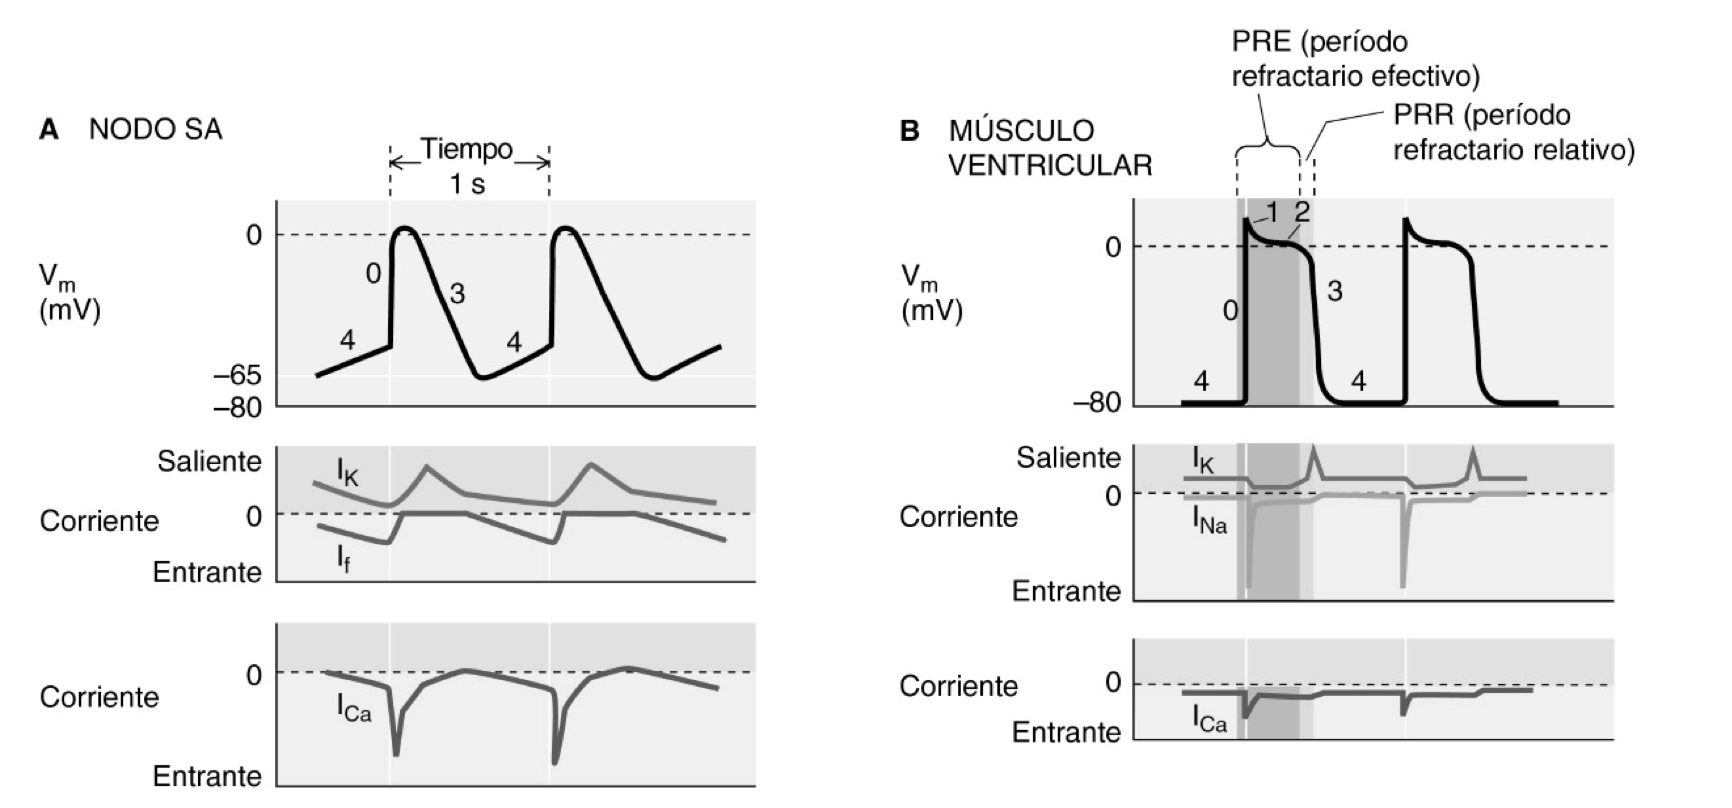
\includegraphics[scale=0.45]{chapters/chapter-02/images/action_potential_phases.png}
  \caption[Fases de los potenciales de acción cardíacos.]{Fases de los potenciales de acción cardíacos. Los
  registros de esta figura son ideales. $I_K$, $I_{Na}$, $I_{Ca}$ e $I_f$ son corrientes a través de canales
  de $K^+$, $Na^+$, $Ca^{2+}$ y catiónicos no selectivos, respectivamente. Figura extraída de \cite{bk:boron3ed}}
  \label{fig:action_potential_phases}
\end{figure}

\subsection{Propagación del impulso} \label{subsec:pulse-propagation}

\indent Existen variaciones regionales en la velocidad de conducción del impulso cardíaco. \\
\indent El retardo de conducción no es proporcional a la distancia recorrida, lo cual indica que la velocidad de
propagación no es uniforme. En contraste con el miocardio ordinario y la vía de conducción rápida, los potenciales
de acción de las células nodales presentan menor amplitud y una fase 0 más lenta porque la corriente de $Ca^{2+}$
constituye el elemento predominante de la excitación. El mayor retardo de conducción se observa entre el nódulo AV y
el haz de His, a pesar de que sólo unos pocos milímetros separan a estas dos estructuras. Esto se debe al hecho de
que un potencial lento genera corrientes locales débiles y, por lo tanto, es menos apto para la conducción. Además,
las uniones intercelulares comunicantes o en hendidura son menos numerosas en el nódulo AV. Aunque cada
miocardiocito está rodeada de una membrana aislante, el miocardio se comporta desde el punto de vista eléctrico como
una célula única gigante (sincicio funcional) debido a la presencia de los discos intercalares. Estos discos son
estructuras que separan las células vecinas e incluyen regiones especializadas en las que las membranas adyacentes
se adosan y que contienen "canales" de gran diámetro. Estos permiten el paso de iones y moléculas de bajo peso
molecular y constituyen vías de baja resistencia eléctrica. Estos canales (no selectivos) conducen la corriente del
circuito local, de manera que el flujo eléctrico que parte del nódulo sinusal se propaga a toda la masa del tejido.

\section{Actividad mecánica} \label{sec:mechanical-activity}

El corazón posee una función de bomba, la cual se cumple mediante la contracción y relajación rítmica del músculo
cardíaco que lo forma. Esta formado por dos corazones, el corazón izquierdo y el derecho. El corazón derecho impulsa
sangre venosa que llega luego de haber atravesado los diferentes órganos. Esta desemboca en la aurícula derecha por
dos grandes venas: cava superior y cava inferior. Pasa a través de la válvula tricúspide al ventrículo derecho y
éste la eyecta por la arteria pulmonar al circuito menor; allí se produce la hematosis. La sangre ya oxigenada y con
una presión parcial de dióxido de carbono ($P_{CO_2}$) normal regresa por las venas pulmonares a la aurícula
izquierda. Desde ella pasa a través de la válvula mitral al ventrículo izquierdo, el cual la expulsará por la aorta
a toda la economía. Las válvulas auriculoventriculares, mitras y tricúspide, aseguran la dirección del flujo
sanguíneo al evitar que durante la sístole la sangre que contienen los ventrículos refluya a las aurículas. Las
válvulas sigmoideas, aórtica y pulmonar, también aseguran la dirección del flujo al impedir que la sangre refluya
desde estos vasos a los ventrículos durante el intervalo diastólico. \\
\indent A pesar que los dos ventrículos poseen un volumen interno similar y expulsan igual cantidad de sangre, el
derecho debe generar unos $15-20$ mmHg de presión par abrir la válvula sigmoidea pulmonar, mientars que el izquierdo
debe generar aproximadamente $80$ mmHg para abrir la sigmoidea aórtica. La fuerza que cada uno de estas cavidades
deben hacer explica los grosores de sus paredes. Cada fibra miocárdica realiza la misma fuerza pero el ventrículo
izquierdo posee una mayor cantidad de estas fibras. \\
\indent Los ventrículos de un adulto promedio expulsan aproximadamente $50$ ml por latido. Sin embargo, dejan un
volumen residual sin esxpulsar, que es igual o ligeramente inferior al expulsado. Por lo tanto, el volumen
ventricular antes de la eyección es de unos $70$ a $80$ ml. Este volumen se denomina \textit{volumen diastólico
final} (VDL) y el porcentaje que se expulsa de este volumen se conoce como \textit{fracción expulsada} (FE). Éste es
de aproximadamente $60-70\%$.

\subsection*{Ciclo cardíaco}

El ciclo cardíaco un proceso continuo y periódico, de frecuencia variable de acuerdo a las necesidades del cuerpo
humano. Este ciclo variará su volumen de eyección, su frecuencia cardíaca dependiendo de eventos externos al sistema
cardiovascular. \\
\indent \textbf{Fase isovolumétrica sistólica}. Llamada anteriormente fase isométrica sistólica, pasó
a denominarse isovolumétrica al apreciarse que durante ella se producían cambios en la forma de cavidades, aunque no
en su volumen. El aumento de la presión intrventricular que se origina cuando comienzan a contraerse las fibras
ventriculares origina el cierre de las válvulas auriculoventriculares. Como las válvulas se encuentran cerradas, el
volumen ventricular no se modifica y por este período se denomina isovolumétrico. La presión intraventricular izquierda
asciende desde aproximadamente 20 mmHg a 80 mmHg en menos de una décima de segundo. Esto proporciona una velocidad
media de desarrollo de la presión intraventricular izquierda de alrededor de 700 $\frac{mmHg}{s}$. Cuando las
presiones intraventriculares alcanzan los niveles de las presiones en la aorta o en la arteria pulmonar las válvulas
sigmoideas se abren y esto marca el fin del periódo isovolumétrico. \\
\indent \textbf{Fase de eyección}. Esta fase comienza al abrirse la válvula sigmoidea correspondiente y finaliza al
cerrarse ésta. \\
\indent Durante este período cada uno de los ventrículos eyecta aproximadamente $50-60$ ml. La eyección de la sangre
esta dada por la contracción de las fibras del miocardio. Las presiones medias con las que debe realizar fuerza los
ventrículos son de $100$ mmHg y $16$ mmHg para el el izquierdo y derecho respectivamente. \\
\indent \textbf{Fase isovolumétrica diastólica}. Una vez que la expulsión finaliza, y que la presión en la aorta o
la pulmonar iguala o supera a la existente en el ventrículo izquierdo o el derecho, las válvulas sigmoideas se
cierran. Como las válvulas auriculoventriculares aún permanecen cerradas, la presión intraventricular disminuirá sin
cambios de volumen. La presión descenderá de forma isovolumétrica hasta que la presión en las aurículas supere a la
ventricular y se abran las válvulas auriculoventriculares. \\
\indent \textbf{Fase de llenado}. La apertura de las válvulas auriculoventriculares señala el inicio de la fase de
llenado, la cual se complementará con la contracción auricular, la cual dará por finalizado a esta fase.

\indent En la Figura \ref{fig:cardiac_cycle} se ilustra el ciclo cardíaco en un gráfico de presión-volumen donde
queda definido claramente los diferentes hitos del ciclo.

\begin{figure}[H]
  \centering
  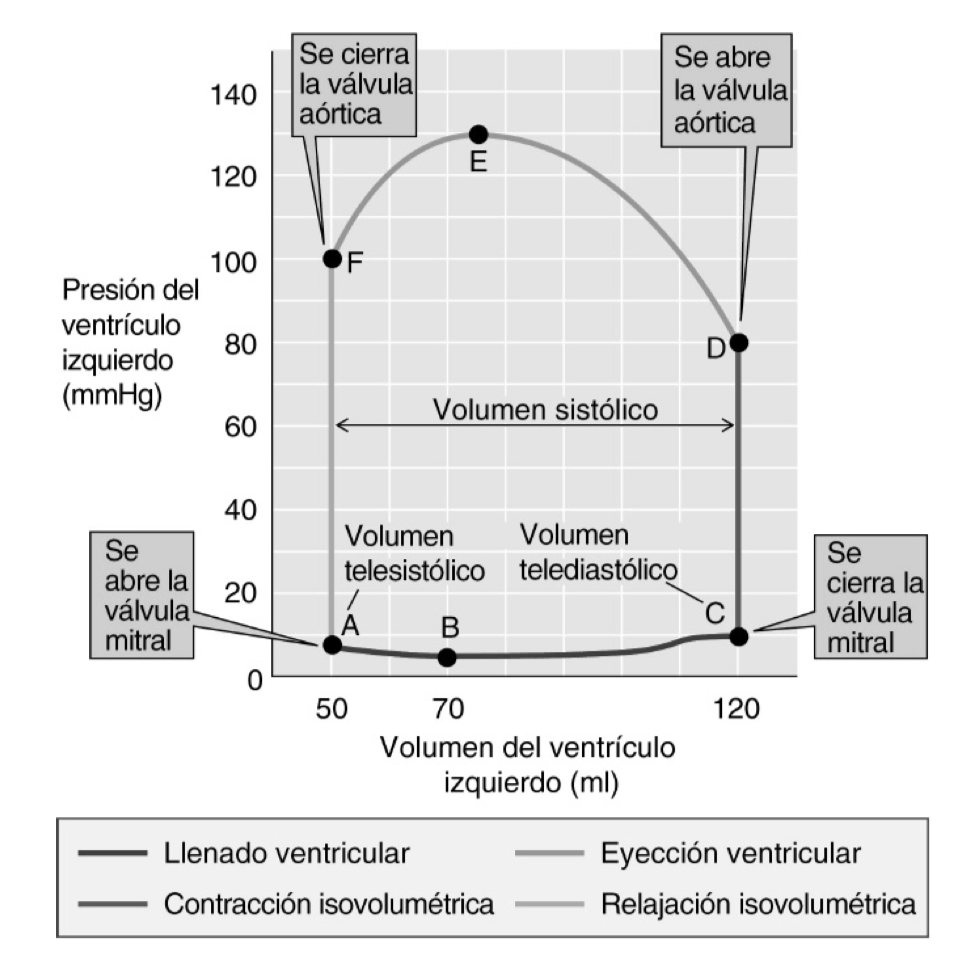
\includegraphics[scale=0.65]{chapters/chapter-02/images/cardiac_cycle.png}
  \caption[Curva de presión-volumen del ventrículo izquierdo.]{Curva de presión-volumen del ventrículo izquierdo.
  Figura extraída de \cite{bk:boron3ed}}
  \label{fig:cardiac_cycle}
\end{figure}

\section{El Fonocardiograma} \label{sec:the-phonocardiogram}

La actividad mecánica del corazón genera movimientos vibratorios en las diferentes estructuras cardíacas que se
propagan hacia la superficie torácica. Algunas de esas vibraciones son identificadas por el oído humano y
constituyen los ruidos cardíacos. Los movimientos vibratorios de menor frecuencia, detectados por la
visualización o por la palpación de expansiones o retracciones en determinadas regiones de la superficie,
configuran los diferentes pulsos.

\subsection{Ruidos cardíacos}\label{subsec:cardiac-sounds2}

En toda la superficie torácica próxima al corazón se auscultan dos ruidos cardíacos, definidos como el primero
($1^o$) y el segundo ($2^o$) ruido. Éstos coinciden con el comienzo y el final de la sístole ventricular,
respectivamente, y brindan una idea secuencial de los fenómenos que ocurren durante el ciclo cardíaco. Con menor
frecuencia se pueden auscultar otros dos ruidos que se reconocen como tercero ($3^o$) y cuarto ($4^o$). \\
\indent \textbf{Primer ruido}. El primer ruido cardíaco se produce por movimientos vibratorios generados en las
válvulas auriculoventriculares (mitral y tricúspide) y en las estructuras próximas a ellas. Las vibraciones tienen
lugar en el momento del cierre valvular y coinciden con el comienzo de la contracción ventricular o sístole
ventricular. \\
\indent En este ruido predominan vibraciones de baja frecuencia que le confieren una característica auditiva
grave. \\
\indent La zona donde se ausculta mejor y se obtiene el mejor registro gráfico del primer ruido es la región
próxima a la punta del corazón y el área correspondiente a la base del esternón. \\
\indent El registro gráfico de ese ruido (intensidad de la frecuencia vibratoria en función del tiempo),
conocido como fonocardiograma, muestra un grupo central de vibraciones con frecuencia vibratoria de 120 a 142 Hz,
precedido y seguido por movimientos vibratorios de frecuencias menores, entre 30 y 100 Hz. El primer ruido tiene una
duración promedio de $0.1-0.12$ s. \\
\indent \textbf{Segundo ruido}. Al cerrarse las válvulas aórtica y pulmonar se generan movimientos vibratorios
que determinan la generación del $2^o$ ruido. La conformación anatómica de esas estructuras le da al segundo ruido
características auditivas diferentes: su duración es menor, entre $0.07-0.10$ s y frecuencias entre $150-170$ Hz. \\
\indent Por razones de proximidad topográfica, y si bien se puede identificar en toda la región anterior del
tórax, el sitio donde se ausculta y registra mejor es a nivel del segundo espacio intercostal, tanto a la izquierda
del esternón como a la derecha.
\indent \textbf{Tercer ruido}. El tercer ruido cardíaco es auscultado en casi todos los niños y adolescentes sin
enfermedad cardíaca; su prevalencia auscultatoria es menor a medida que aumenta la edad en individuos sanos (23\% en
una población de ambos sexos entre 36 y 37 años de edad). \\
\indent La presencia de este rudio está directamente vinculada a las vibraciones de la pared ventricular durante
el llenado ventricular rápido. \\
\indent \textbf{Cuarto ruido}. El cuarto ruido, también de auscultación poco frecuente en adultos sanos,
coincide con la última parte del llenado ventricular, secundaria a la contracción auricular. Es precedido por la
onda P del registro del electrocardiograma y sigue inmediatamente la contracción auricular. Esto se puede observar
en la Figura \ref{fig:diagrams_in_phase}.

\begin{figure}[H]
  \centering
  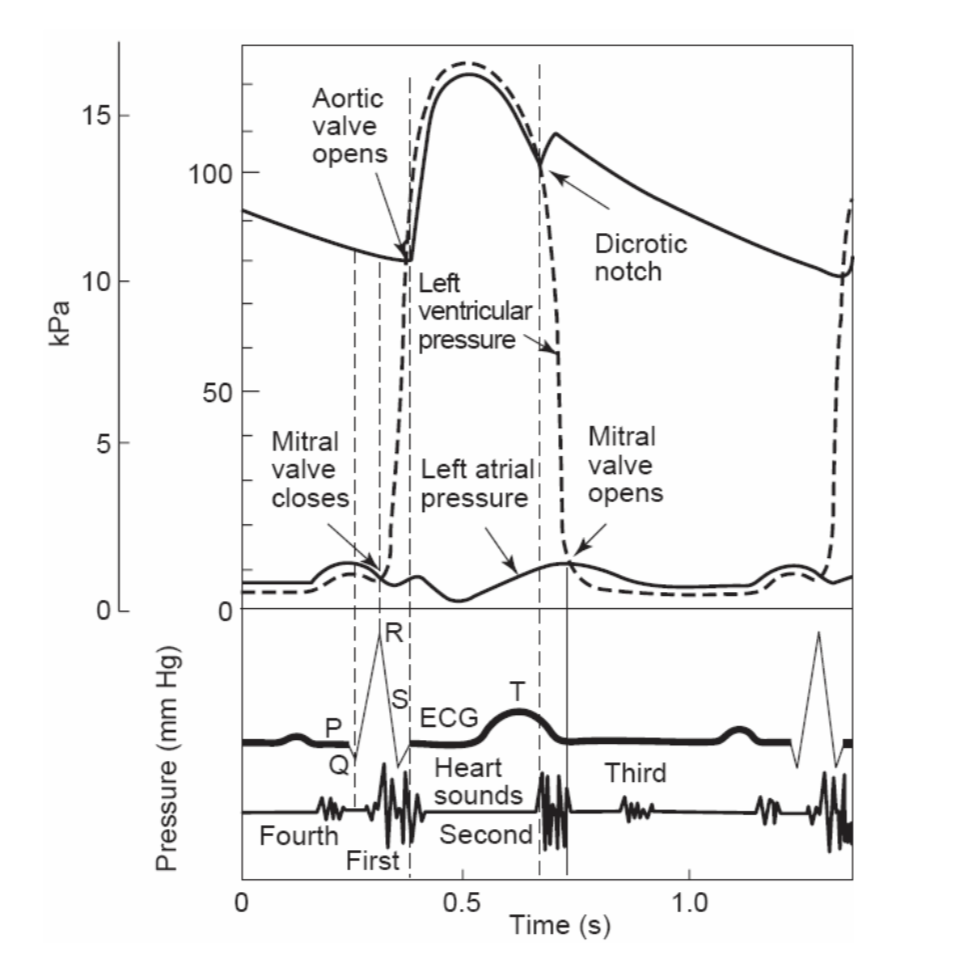
\includegraphics[scale=0.65]{chapters/chapter-02/images/diagrams_in_phase.png}
  \caption[Correlación de los cuatro sonidos cardíacos con los eventos eléctricos y mecánicos del
  cíclo cardíaco en fase.]{Correlación de los cuatro sonidos cardíacos con los eventos eléctricos y
  mecánicos del cíclo cardíaco en fase. Figura extraída de \cite{pp:abbas2014}.}
  \label{fig:diagrams_in_phase}
\end{figure}

\indent El Cuadro \ref{tab:cardiac_sounds} resume los tipos y las características de los ruidos cardíacos. La
identificación de los ruidos cardíacos normales que determinan la sístole y la diástole es la base de la
auscultación. Dicho esto, resulta de suma importancia tener perfectamente caracterizada a la señal que surge de la
auscultación o fonocardiografía.


\begin{table}[H]
  \centering
  \begin{tabular}{ |llll| }
    \hline
    \thead{RUIDO} & \thead{LOCALIZACIÓN \\ EN EL CICLO \\ CARDÍACO}  & \thead{MECANISMO}  & \thead{IMPLICACIÓN
    \\ CLÍNICA}  \\
    \hline
    \thead{4$^{to}$ ruido} & \thead{Presistólico, antes del \\ 1$^{er}$ ruido} & \thead{Contracción enérgica \\
    de aurícula} & \thead{Patológico, HTA, \\ alteración de la \\ distensibilidad del \\ VI o del VD} \\
    \thead{1$^{er}$ ruido} & \thead{Inicio de la \\ sístole ventricular} & \thead{Cierre de válvulas AV} &
    \thead{Fisiológico si \\ es normal} \\
    \thead{Clics \\ mesotelesistólicos} & \thead{Mesotelesistólicos} & \thead{Desplazamiento posterior \\ hacia
    aurícula \\ de valvas mitrales \\ (posterior)} & \thead{Patológicos. \\ Aislados o antes \\ de soplos
    sistólicos \\ por insuficincia \\ mitral}\\
    \thead{2$^{do}$ ruido} & \thead{Fin de la sístole} & \thead{Cierre de válvulas \\ sigmoideas, aórtica y \\
    pulmonar} & \thead{Fisológico \\ si es normal} \\
    \thead{Chasquidos de \\ apertura} & \thead{Inicio de la diástole, \\ después del 2$^{do}$ ruido. \\ Inicio
    de la sístole, \\ después del 1$^{er}$ ruido} & \thead{Apertura de la \\ válvula AV enferma \\ (reumática),
    aperturas \\ sigmoideas enfermas} & \thead{Patológicos. Estenosis \\ mitral y tricuspídea. \\ Estenosis
    aórtica y \\ pulmonar} \\
    \thead{3$^{er}$ ruido} & \thead{Protodiastólico} & \thead{Distensión ventricular súbita \\ en la fase de
    llenado rápido} & \thead{Fisiológico en niños \\ y adultos jóvenes. \\ Patológico en el resto.} \\
    \hline
  \end{tabular}
  \vspace{0.5ex}
  \raggedright \textit{\footnotesize VI: Ventrículo Izquierdo; VD: Ventrículo derecho; HTA: Hipertensión
  arterial; AV: auriculoventricular.}
  \caption{Tipos y características de los sonidos cardíacos.}
  \label{tab:cardiac_sounds}
\end{table}

\subsection{Estado del arte} \label{subsec:state-of-the-art}

A partir de esto surgieron propuestas de procesar, clasificar y segmentar las señales derivadas del
fonocardiograma. El PCG es una onda mecánica, particularmente sonido, que refleja el proceso del corazón como
bomba cardíaca y en ella queda asentado el correcto funcionamiento del corazón, esto ya sea las válvulas
cerrándose correctamente, el ritmo cardíaco, rigidez de las paredes cardiovasculares, entre otras
características. \\
\indent Aquí surgen varios desafíos. La clasificación de patologías cardíacas asociadas y segmentación de la
señal en sus sonidos fundamentales. Todo esto en la práctica, al realizar la adquisición de estas señales se
encuentra contaminado de distintos factores, externos al fonocardiograma. Estas fuentes de ruido pueden ser de
naturaleza eléctrica, como la tensión de línea de $50-60$ Hz (dependiendo de la zona geográfica) o mecánica como el
habla. Otros ejemplos contaminación es la respiración (de baja frecuencia), produce que la línea isoeléctrica se
perciba como oscilante. Por otro lado, puede haber presencia de ruido muscular. \\
\indent Hasta la actualidad varias personas han trabajado con estos problemas, ya sea tanto clasificación como
segmentación. Liang et al. en \cite{pp:liang}, han trabajado con algoritmos determinísticos basados en la detección
de picos con la energía y envolvente de Shannon. Esto ha mostrado una performance interesante pero ante señales muy
corruptas puede haber picos que interfieran con la detección y reduzcan la eficiencia de detección de los sonidos
fundamentales. Luego, un segundo trabajo en \cite{pp:liang2} se utilizó la descomposición de wavelet y la energía de
Shannon para detectar los picos en cada bloque y realizar la segmentación, así obteniendo una vez más performance
altas aunque similares al trabajo anterior. \\
\indent En 2010, Schmidt \textit{et al.} \cite{pp:schmidt2010} han propuesto un sistema de segmentación donde
proponen el algoritmo \acrshort{dhmm} (\textit{Duration-dependant Hidden Markov Model}) logrando un alto desempeño a
la hora de la clasificación de los sonidos fundamentales tanto para pacientes sanos como enfermos. Luego, en 2014,
Abbas \textit{et al.} \cite{pp:abbas2014} han propuesto una técnica de clasificación basada en \textit{K-means
clustering} mostrando una alta estabilidad en la detección y clasificación, donde juega un rol vital en la
cuantificación e identificación de diferentes casos hemodinámicos. Hasta 2015, los distintos métodos de clasificación
debían estar acompañadas por señales adicionales como el ECG. En 2015, David Springer \textit{et al.}
\cite{pp:springer2015} han publicado un algoritmo de segmentación de los sonidos S1 y S2 con un sólo canal de PCG
sin referencia externa usando una modificación del algoritmo propuesto por Schmidt, así mejorando la perfomance del
estado del arte. \\
\indent Recientemente, Franceso Renna y Miguel Coimbra de la Universidad de Porto, Portugal, propusieron el uso
de \acrshort{cnn} (\textit{Convolutional Neural Network}). Este enfoque fue utilizado en otros trabajos para la
segmentación de imágenes. Asimismo, aplicaron a la salida de diferentes modelos temporales que generan una salida
consistente y que responde a la naturaleza de transición de los estados del fonocardiograma, mejorando las métricas
del trabajo de Springer.
    
  \chapter{Estudio de bases de datos} \label{ch:databases-study}

La selección de datos para la implementación del segmentador se extrajo de \textsc{PhysioNet}, organización apoyada
por \textit{National Institute of General Medical Sciences} (\acrshort{nigms}) y \textit{National Institute of
Biomedical Imaging and Bioengineering} (\acrshort{nibib}). Esta organización se dedica a ofrecer, de manera
gratuita, acceso a un gran cantidad de señales fisiológicas y herramientas para el procesamiento de las mismas. \\
\indent Particularmente, se extrajeron dos base de datos. Una asociada a un desafío público en el año 2016 que se
denominaba ``\textit{Classification of Normal/Abnormal Heart Sound Recordings: the PhysioNet/Computing in Cardiology
Challenge 2016}``, el cual consistía en diseñar e implementar un clasificador de fonocardiogramas normales y
anormales bajo ciertas condiciones. En el Cuadro \ref{tab:challenge2016} se mencionan las características generales
de la base de datos.

\begin{table}[H]
  \centering
  \begin{tabular}{ |c|c|c|c|c|c|c| }
    \hline
    \thead{Set} & \thead{Cantidad \\ de archivos} & \thead{Normal} & \thead{Anormal} & \thead{Duración \\
    promedio [s]} & \thead{Máx. \\ duración [s]} & \thead{Mín. \\ duración [s]} \\
    \hline
    \thead{training-a} & \thead{409} & \thead{117} & \thead{292} & \thead{32.56} & \thead{36.5} & \thead{9.27} \\
    \thead{training-b} & \thead{490} & \thead{386} & \thead{104} & \thead{7.98} & \thead{8} & \thead{5.31} \\
    \thead{training-c} & \thead{31} & \thead{7} & \thead{24} & \thead{49.44} & \thead{122} & \thead{9.65} \\
    \thead{training-d} & \thead{55} & \thead{27} & \thead{28} & \thead{15.15} & \thead{48.54} & \thead{6.61} \\
    \thead{training-e} & \thead{2141} & \thead{1958} & \thead{183} & \thead{23.07} & \thead{101.67} & \thead{8.06} \\
    \thead{training-f} & \thead{114} & \thead{34} & \thead{114} & \thead{33.12} & \thead{59.62} & \thead{29.38} \\
    \hline
  \end{tabular}
  \caption[Base de datos: Challenge 2016]{Base de datos: Challenge 2016. Tipos y características de los sonidos
  cardíacos.}
  \label{tab:challenge2016}
\end{table}

\indent Señales recolectadas en ambientes clínicos y no clínicos, y de pacientes sanos y patológicos. El total es de
3126 fonocardiogramas para el set de entrenamiento (sólo el set A viene acompañado de señales del \acrshort{ecg} y
300 fonocardiogramas para el set de validación. \\
\indent Estos fonocardiogramas fueron extraídos del área aórtica, área pulmonar, área tricúspide y mitral. En cada
subset de datos, se clasificaron en fonocardiogramas normales y anormales. Los fonocardiogramas normales fueron
extraídos de pacientes sanos y los anormales de pacientes con problemas cardíacos. Los pacientes sufren de distintas
enfermedades cardíacas que no se encuentran detalladas en cada uno de los pacientes. Sin embargo, las enfermedades
cardíacas típicas son deficiencias valvulares y enfermedades asociadas a las coronarias. Las deficiencias valvulares
incluyen prolapso de la válvula mitral, regurgitación mitral, estenosis aórtica y cirugías valvulares. Todos los
pacientes sanos y patológicos incluyen adultos y niños, y cada uno de éstos pueden aportar de uno a seis grabaciones.
Adicionalmente, cada una de las grabaciones fue muestreada a 2000 Hz y una única derivación del fonocardiograma. \\
\indent Es importante tener en cuenta, dado que las grabaciones fueron hechas en ambientes no controlados, muchas
de éstas se encuentan contaminadas por diferentes fuentes de ruido, como el habla, movimiento del estetoscopio,
respiración y ruidos intestinales. \\
\indent La segunda base de datos ha sido publicada por David Springer a partir del trabajo en \cite{pp:springer2015}
. Si bien no es exactamente la base de datos utilizada en su trabajo, fue aportada por él junto a una implementación
hecha en \textsc{MATLAB\texttrademark}. \\
\indent A diferencia de la base del \textit{Challenge 2016}, posee 792 grabaciones de fonocardiogramas muestreadas a
una frecuencia de 1000 Hz. Éstas fueron extraídas de 135 pacientes, y más de una grabación por paciente. También, se
han dividido grabaciones en varias secciones por inconsistencias de anotaciones. \\
\indent Las anotaciones están basadas en electrocardiogramas (no presentes en el set de datos), las cuales
involucran la onda R y el fin de la onda T muestreadas a 50 Hz. Estas anotaciones fueron extraídas de manera
automática mediante un método de concordancia, el cual se detallará en la Sección \ref{sec:annotations}. \\
\indent Por otro lado, se utilizó una clasificación binaria para definir cada grabación como patológica o no
patológica.

\section{Selección y normalización de datos} \label{sec:data-selection-normalization}

Ya vimos que estas bases de datos contienen datos que difieren entre si. Desde la cantidad de señales hasta los tipos
de datos (\acrshort{ecg}, anotaciones del \acrshort{ecg}, frecuencia de muestreo). \\
\indent Dicho esto es necesario decidir por una base de datos en una primera instancia. Para ponerlo en términos
cuantitativos se menciona el por qué de la elección de una base respecto de la otra. La frecuencia de
muestreo no es un problema, por lo tanto tanto 1 KHz como 2 KHz es más que suficiente para tener una buena
resolución en tiempo. Ambas bases clasifican las señales respecto a si son patológicas o no patológicas, es decir,
que es posible realizar algún tipo de entrenamiento para la clasificación de éstas, aunque no es el alcance de este
trabajo y no afecta a la selección de los datos. Sin embargo, esto sirve para identificar que la base no se
encuentre desbalanceada respecto a la proporción de sanos como enfermos. El punto crítico de la selección de la base
se debe a las anotaciones del electocardiograma. La base de datos de Springer \cite{ref:logi-regression-springer} ya
contiene marcas extraídas automáticamente y filtradas por un algoritmo de concordancia. De lo contrario, en la base
de datos del desafío se proveen los \acrshort{ecg}, a los cuales es necesario extraerles las marcas correspondientes.
Debido a que el alcance del trabajo es implementar un segmentador de PCG y no un extractor de anotaciones, se optó
por utilizar la base de David Springer dado que permite apoyarse sobre trabajos previos que ya han utilizado
dichos datos, confiando en la naturaleza de estos datos y así realizar una mejor comparación en el Capítulo
\ref{ch:results}.
Asimismo, se referirá a la base seleccionada como \textit{base de datos} para evitar confusión. \\
\indent Los datos de la base de datos se encuentran en formato \texttt{.mat} (formato propietario de
\textsc{MATLAB\texttrademark}) y las anotaciones de las ondas R y fin de la T, se encuentran muestreadas a 50 Hz.
Esto requiere estandarizar el formato de los datos y acomodar la frecuencia de las anotaciones dado que las
señales se encuentran a una frecuencia de muestreo mayor. Para ello, se tomó como estándar el formato
\acrshort{wfdb} (\textit{Waveform Database}), el cual contiene dos categorías estándar, \textit{MIT Format} y
\textit{EDF Format}.

\subsection*{MIT Format}
\begin{itemize}
  \item Los archivos \textit{MIT Signal} (\texttt{.dat}) son archivos binarios que contienen muestras de señales
  digitalizadas. Éstas almacenan las señales, pero no pueden ser interpretados sin los \textit{header} files.
  Los archivos son de la forma: \texttt{\{RECORD\_NAME\}.dat}.
  \item Los archivos \textit{MIT Header} (\texttt{.hea}) son archivos de texto cortos que describen el contenido
  del archivo de la señal asociado.
  \item Los archivos \textit{MIT Annotation} son archivos binarios que contienen anotaciones (etiquetas que
  generalmente refieren a muestras específicas de una señal asociada). Éstos deben ser leídos junto a los archivos
  \textit{header} asociado. En caso de que en un directorio se vean archivos \texttt{\{RECORD\_NAME\}.dat}, y/o
  \texttt{\{RECORD\_NAME\}.hea}, cualquier otro archivo con otra extensión es un archivo de anotaciones. Por ejemplo,
  \item \texttt{\{RECORD\_NAME\}.atr} es un archivo con anotaciones para esa señal.
\end{itemize}

\subsection*{EDF Format}
\begin{itemize}
  \item Los archivos \href{http://www.edfplus.info/specs/edf.html}{\underline{EDF}} contienen señales digitalizadas almacenadas en formato internacional. Estos archivos guardan la información de encabezado al comienzo del archivo, a diferencia del formato MIT. A su vez pueden estar acompañados de archivos con anotaciones.
  \item Por ejemplo, si existe un archivo \texttt{*.edf}, un archivo con anotaciones asociado podría ser \texttt{*.edf.qrs}, donde \texttt{.qrs} es la extensión de las anotaciones en este caso (podría ser otro).
  \item Los archivos \href{http://www.edfplus.info/specs/edfplus.html}{\underline{EDF+}} son archivos EDF que contienen anotaciones codificadas como señales.
\end{itemize}

\indent La categoría utilizada en este trabajo es \textit{MIT Format}. Este formato debe ser leído con una libreria
especializada. \textit{WFDB Software Package} es un conjunto de funciones para escribir y leer en formatos
específicos de \textit{PhysioBank databases} (entre otros). La libreria \textit{WFDB} es \textit{LGPLed}, y puede
ser usada para programas escritos en \textit{ANSI/ISO C}, \textit{K\&R C}, \textit{C++}, o \textit{Fortran},
corriendo bajo sistemas operativos para los cuales el compilador \textit{ANSI/ISO} or \textit{K\&R C} se encuentre
disponible, incluyendo todas las versiones Unix, MS-DOS, MS-Windows, the Macintosh OS, y VMS. Opcionalmente, la
librería de WFDB puede ser compilada con HTTP o FTP como input sin tener que bajar localmente toda la base de datos
para un procesamiento. \\
\indent En este trabajo se utilizó \textit{WFDB Toolbox for MATLAB\texttrademark}, el cual provee acceso desde
\textsc{MATLAB\texttrademark} a las aplicaciones de \texttt{WFDB}. Esta toolbox provee \textsc{MATLAB\texttrademark} y
Java
\textit{wrappers} para las distintas aplicaciones y un instalador que instala la toolbox en sí misma y el
\textit{WFDB Software Package} precompilado. Esta toolbox corre en 64-bit \textsc{MATLAB\texttrademark} R2010b o
mayor en \textit{GNU/Linux}, \textit{Mac OS X}, y \textit{MS-Windows}. \\
\indent El set de datos de Springer, fue convertido de \textit{MAT Format} a \textit{MIT Format}, donde el
directorio tiene la estructura de la Figura \ref{fig:springer-db}. Los archivos \texttt{.dat} contienen la señal del
PCG. La información ejemplo de los archivos \texttt{.hea} se observan en la Figura \ref{fig:hea-info} y los archivos
\texttt{.ann} contienen las anotaciones de las ondas R y el fin de la T, de acuerdo al estándar provisto por
\textsc{PhysioNet}.

\begin{figure}[H]
  \centering
  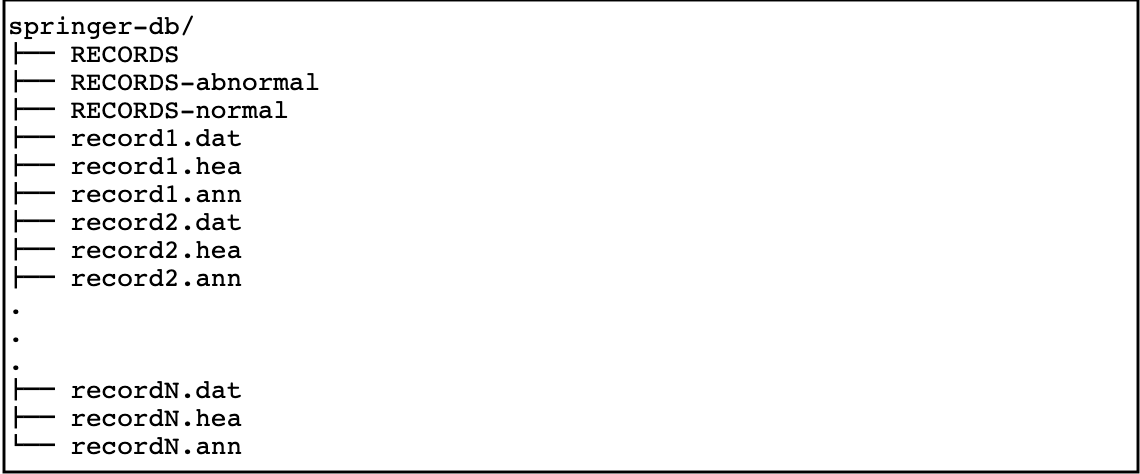
\includegraphics[scale=0.73]{chapters/chapter-03/images/springer-db.png}
  \caption[Estructura del directorio de la base de datos.]{Estructura del directorio de la base de datos. El
  archivo \texttt{RECORDS} contiene en un archivo de texto los nombres de la señales del set de datos, lo mismo
  para \texttt{RECORDS-abnormal} y \texttt{RECORDS-normal}, asociados a señales patológicas y no patológicas
  respectivamente.}.
  \label{fig:springer-db}
\end{figure}

\begin{figure}[H]
  \centering
  
\includegraphics[scale=0.74]{chapters/chapter-03/images/hea-info.png}
  \caption[Información ejemplo del archivo header de una señal]{Información ejemplo del archivo header de una
  señal. En la primer línea se encuentra, de forma ordenada, el nombre de la señal, la cantidad de señales en el
  archivo \texttt{.dat}, la frecuencia de muestreo en Hz y la cantidad de muestras. La segunda línea contiene el
  nombre del archivo y a continuacíon información de adquisción.}
  \label{fig:hea-info}
\end{figure}

\indent En cuanto a la corrección de las anotaciones provistas en la base de datos que se encuentran submuestreadas
a 50 Hz. Para ello, se recupera la frecuencia original a partir de la ecuación \ref{eq:adapt-annotations}.

\begin{align}
  \label{eq:adapt-annotations}
  \bm{a}_{f_2} = \frac{f_2}{f_1} \cdot \bm{a}_{f_1}
\end{align}

\indent Donde $f_1 = 50$ Hz y $f_2 = 1000$ Hz.

  \chapter{Preprocesamiento} 

\section{Acondicionamiento de la señal}

Las señales biológicas, como tantas otras, presentan contaminación en el momento de la adquisición. Éstas fuentes de ruido, ya las mencionamos antes, provienen de ruidos respiratorios, intestinales, habla, entre otras. Por varios motivos es recomendable realizar un pre-procesamiento de ellas para que los algoritmos que buscan características específicas de la señal en cuestión no "se confunda". Por ejemplo, los algoritmos de delineado de \acrshort{ecg}, donde ubican las ondas fundamentales (P, Q, R, S, T$_{on}$, T, T$_{off}$) mejor se desempeñan cuanto más limpia o clara es la señal. \\
\indent Un fonocardiograma presenta frecuencias entre $25-250$ Hz. Esto se debe a los sonidos fundamentales de la señal, S$_1$ y S$_2$. El contenido espectral de S$_1$ se encuentra entre $10-180$ Hz, mientras que S$_2$ entre $50-250$ Hz. En el primer caso, la mayor energía espectral se encuentra en componentes por debajo de los 130 Hz. Por supuesto, que la presencia de otras frecuencias que no son intrínsecas al fonocardiograma pueden estar relacionado a enfermedades de insuficiencia cardíaca como contaminación del entorno. \\
\indent Para realizar el filtrado se utilizaron dos filtros lineales e invariantes en el tiempo de respuesta infinita al impulso. Un Butterworth pasa-altos y pasa-bajos. Las características de estos filtros se detallan más adelante. Esta etapa es importante dado a que elimina ruido de contenido alto en frecuencias, que se observa un "pasto" sobre la señal, y también remueve contenido de baja frecuencia que genera lo que se conoce como línea de base móvil (\textit{baseline wandering}), causado por contenido de baja frecuencia como la respiración. Lo que ocurre es que la línea isoeléctrica (\textit{baseline}) se encuentra desnivelada. Por otro lado, se remueve el valor medio (\textit{offset}). A pesar del filtrado, algunas señales contienen ruido de baja frecuencia que no es posible eliminar con filtros lineales, de esta forma, se aplica el algoritmo de media móvil (\textit{moving vverage}) con una ventana de largo determinado heurísticamente para suavizar los picos. También se aplica un algoritmo de eliminación de picos de los fonocardiogramas. Finalmente, se termina normalizando las señales para que contengan energía unitaria. \\
\indent A continuación se observan las especificaciones de los filtros. En la Figura \ref{fig:high-pass} y \ref{fig:low-pass} se ilustran las magnitudes de los filtros y las fases, y en la Figura \ref{fig:high-pass-tb} y \ref{fig:low-pass-tb} las bandas de transición.

\begin{table}[H]
\centering
\begin{tabularx}{\textwidth}{|X|l|l|l|l|l|l|}
	\hline 
    \textbf{Filtro} & \textbf{Orden} & \textbf{A}$_+$ & \textbf{A}$_-$ & $\omega_c$ & $\omega_+$ & $\omega_-$  \\
    \hline
    \thead{Pasa-altos} & \thead{4} & \thead{0.01} & \thead{0.01} & \thead{25 Hz} & \thead{41 Hz} & \thead{1.5 Hz} \\        
    \hline
    \thead{Pasa-bajos} & \thead{4} & \thead{0.01} & \thead{0.01} & \thead{400 Hz} & \thead{467 Hz} & \thead{345 Hz} \\        
    \hline
    
\end{tabularx}

\caption[Tabla de especificaciones de los filtros]{Tabla de especificaciones de los filtros. A$_+$ es la atenuación de la banda de paso, \textbf{A}$_-$ la atenuación de la banda de rechazo, $\omega_c$ la frecuencia de corte, $\omega_+$ la frecuencia de paso y $\omega_-$ la frecuencia de rechazo.}

\end{table}

\pagebreak

\begin{figure}[H]
    \centering
    \begin{subfigure}[b]{\textwidth}
        \centering
        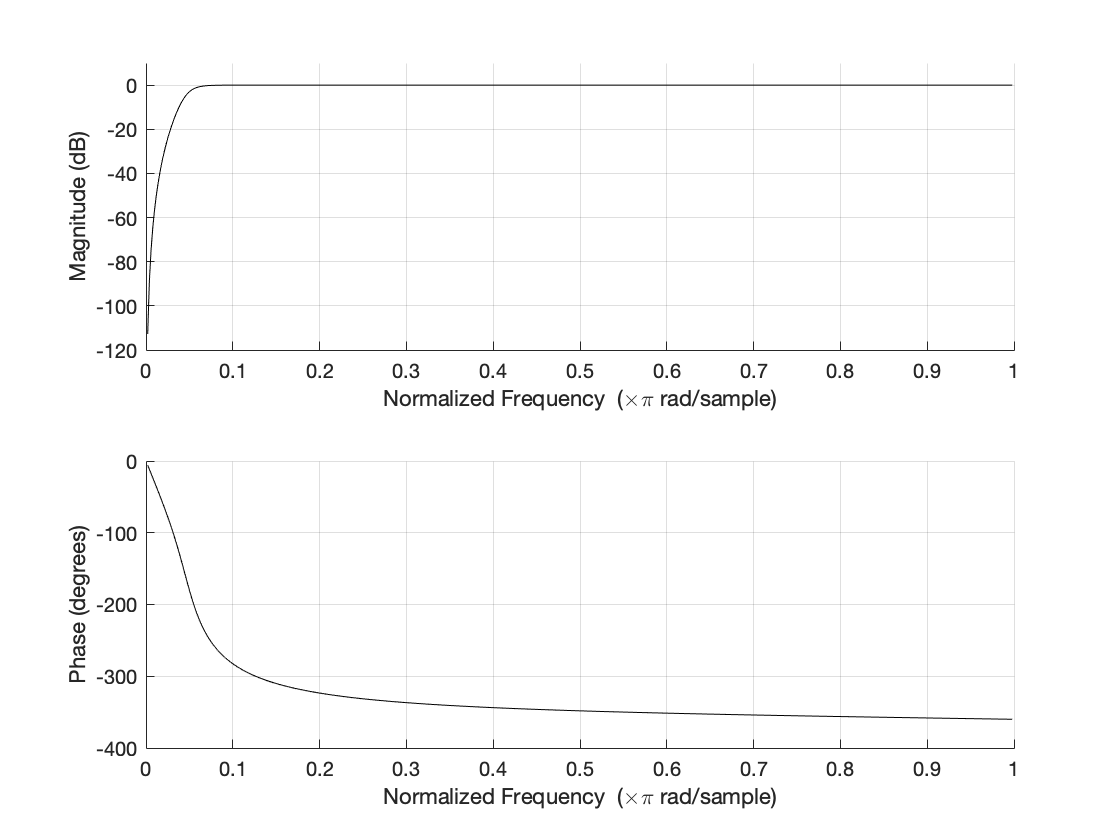
\includegraphics[scale=0.35]{sections/chapter-04/images/high-pass.png}
        \caption[Magintud y fase del filtro pasa-altos]{Magintud y fase del filtro pasa-altos.}
        \label{fig:high-pass}
    \end{subfigure} \\
    \begin{subfigure}[b]{\textwidth}
        \centering
        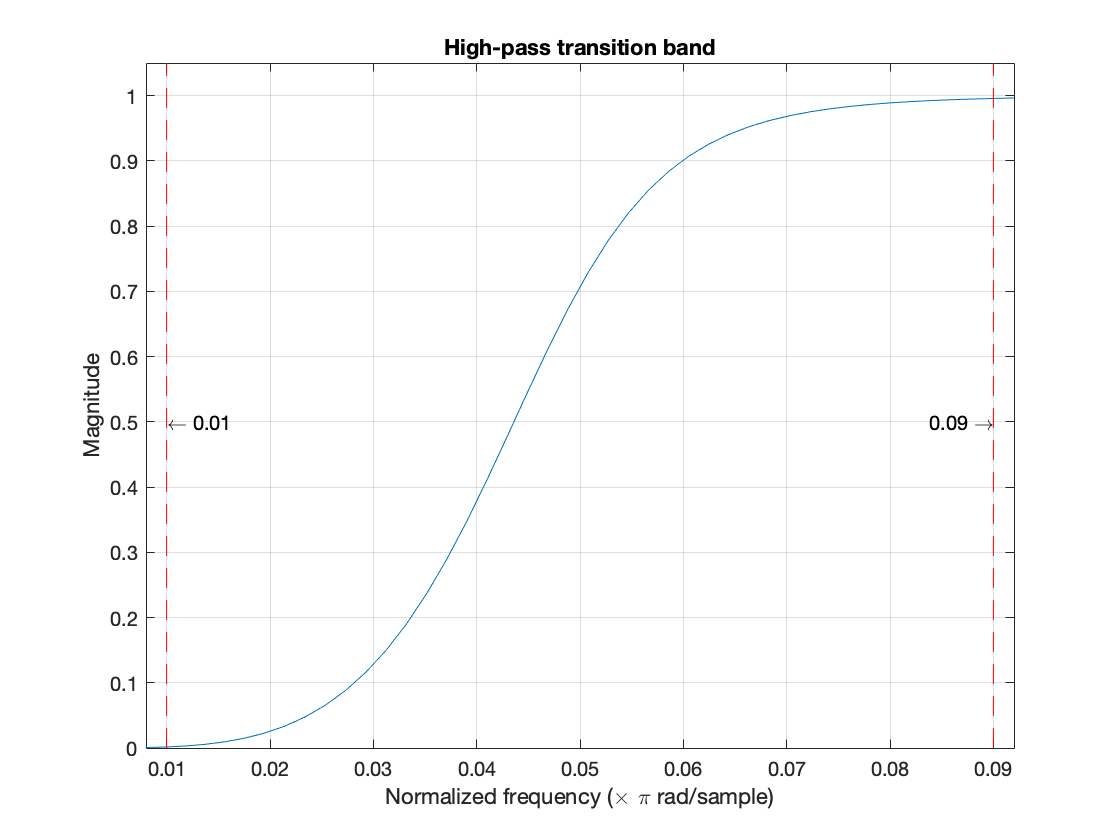
\includegraphics[scale=0.35]{sections/chapter-04/images/high-pass-tb.png}
        \caption[Banda de transición del filtro pasa-altos]{Banda de transición del filtro pasa-altos.}
        \label{fig:high-pass-tb}
    \end{subfigure}
    \caption[Filtro pasa-altos]{Filtro pasa-altos.}
\end{figure}

\begin{figure}[H]
    \centering
    \begin{subfigure}[b]{\textwidth}
        \centering
        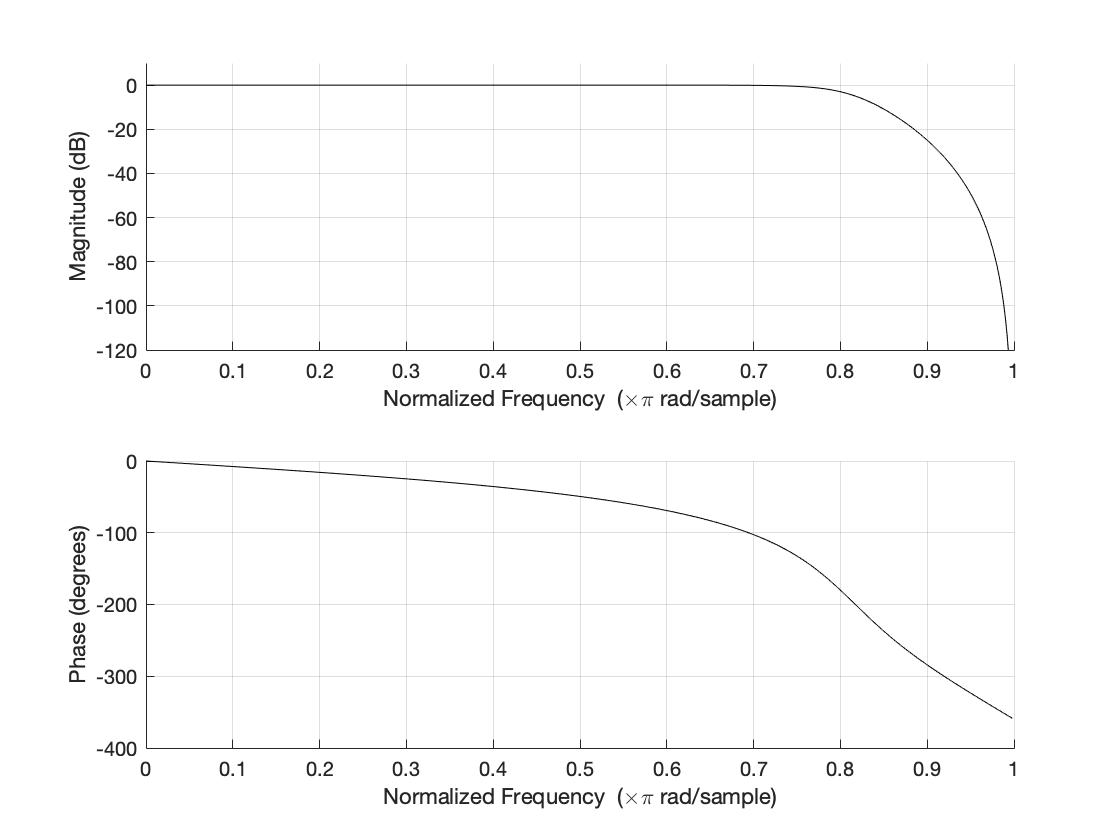
\includegraphics[scale=0.35]{sections/chapter-04/images/low-pass.png}
        \caption[Magintud y fase del filtro pasa-bajos]{Magintud y fase del filtro pasa-bajos.}
        \label{fig:low-pass}    
    \end{subfigure} \\
    \begin{subfigure}[b]{\textwidth}
        \centering
        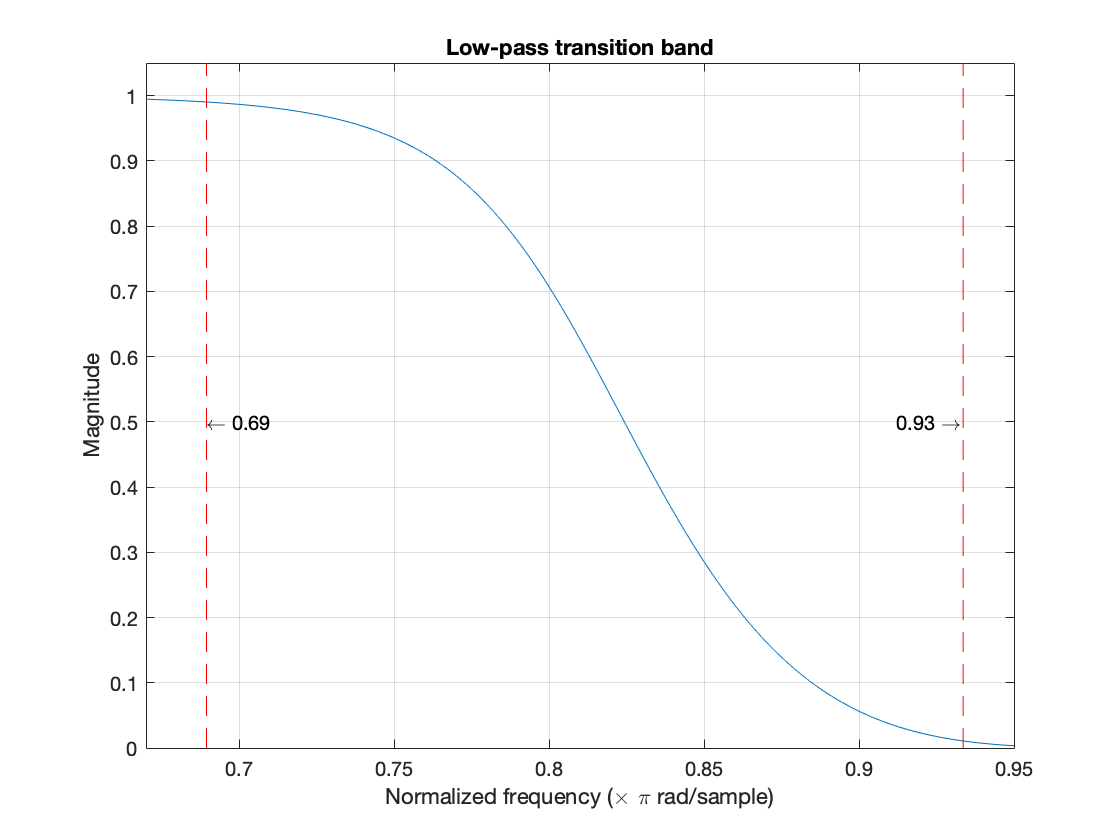
\includegraphics[scale=0.35]{sections/chapter-04/images/low-pass-tb.png}
        \caption[Banda de transición del filtro pasa-bajos]{Banda de transición del filtro pasa-bajos.}
        \label{fig:low-pass-tb}
    \end{subfigure}
    \caption[Filtro pasa-bajos]{Filtro pasa-bajos.}
\end{figure}

\pagebreak

\subsubsection*{Eliminación de picos de fricción}

\indent Los picos de fricción deben ser eliminados dado que estos picos generalmente pueden tener mayor amplitud que los sonidos fundamentales del fonocardiograma. A continuación se presenta el algoritmo para realizar dicho procesamiento. \bigskip

\indent Dada una señal de fonocardiograma $\bm{x}_i \in \mathbb{R}^N$ muestreada a una frecuencia de muestreo $F_s$, se elige una ventana de largo arbitrario, i.e. $L = \left[\frac{F_s}{2}\right]$. \bigskip

\indent La idea fundamental es dividir el \acrshort{pcg} en ventanas de longitud $L$. Debido a esto si el módulo entre la longitud de la señal y el largo de la ventana definido no es cero, algunas muestras quedarán fuera de alguna de las ventanas. Estas muestras se denominan muestras residuales que no participan en el algoritmo y deben ser agregadas al final para recuperar la señal. El número de muestras residuales se definen en la siguiente ecuación. 

\begin{align}
    r_s = \mathrm{mod}(N,L)
\end{align}

\indent Definimos la ventana $\bm{w}_i \in \mathbb{R}^L$, con $i = 0,1,\dots,\left\lfloor \frac{N}{L} \right\rfloor$. Luego, definimos al vector de los máximos, $\bm{m} \in \mathbb{R}^{\left\lfloor \frac{N}{L} \right\rfloor}$. Este vector contiene los valores máximos de las ventanas, denominados \textit{Maximum Absolute Amplitude} (\acrshort{maa}).

\begin{align}
    m_i = \mathrm{max} \; \bm{w}_i 
\end{align}

\indent Las componentes $m_i$ dinámicamente irán cambiando de valor hasta que ninguna de ellas sea superior a 3 veces la mediana de $\bm{m}$. Esta es la condición donde el algoritmo reconstruye la señal filtrada. \bigskip

\indent Hasta que no se cumpla la condición antes mencionada, se busca entre las ventanas la que contenga el mayor pico. 

\begin{align}
    i_{\bm{w}} = \arg \underset{i}{\mathrm{max}} (\bm{m})
\end{align}

\indent Una vez hecho esto es necesario encontrar la posición del pico en la ventana asociada.

\begin{align}
    i_{spike} = \arg \underset{i}{\mathrm{max}} (\bm{w}_{i_{\bm{w}}})
\end{align}

\indent El índice $i_{spike}$ hace referencia al valor máximo del pico de fricción. Sin embargo, es necesario computar el comienzo y el fin del pico para eliminarlo. Para ello se necesitan computar los cruces por cero.

\begin{align}
    s_i = sgn(w_i)
\end{align}

\indent Donde $s_i$ son las componentes del vector que $\mathbf{s}_i \in \mathbb{R}^L$. Luego, se computan los cruces por cero, $\mathbf{z} \in \mathbb{R}^{L-1}$ en la ecuación \ref{eq:zero-crossings}

\begin{align} \label{eq:zero-crossings}
    z_i = s_i - s_{i-1}, \quad 0 \leq i \leq L-2
\end{align}

\indent A partir de este momento sólo queda definir el inicio y el fin del pico. El inicio del pico se encuentra a partir del último cruce por cero hasta la posición $i_{spike}$. El final del pico, se encuentra con el primero cruce por cero despuées de $i_{spike}$. Las ecuaciones \ref{eq:spike-start} y \ref{eq:spike-end} reflejan el cálculo.

\begin{align} \label{eq:spike-start}
    p = \mathrm{max}\big\{n \in \mathbb{N}_0 \; | \; n \leq i_{spike}-1\big\}
\end{align}

\begin{align} \label{eq:spike-end}
    q = \mathrm{min}\big\{n \in \mathbb{N}_0 \; | \; i_{spike} \leq n \leq L-2\big\}
\end{align}

\indent Es posible que el vector de cruces por cero sea nulo, con lo cual los valores de $p$,$q$ deberían coincidir con el primer índice de la ventana y el último respectivamente. Luego, simplemente queda por eliminar este pico.

\begin{align}
    w_{i,j} = \epsilon, \quad p \leq j \leq q
\end{align}

\indent Siendo $\epsilon$ un número tan chico como sea defina. Por último, queda por recalcular el vector $\mathbf{m}$ con $\mathbf{w}_i$ actualizado. \bigskip

\indent Cuando se cumpla la condición de 3 veces la mediana de $\mathbf{m}$, se concatenan todas las ventanas y se agregan al final las muestras residuales. \bigskip

\subsubsection*{Suavizador - Media móvil}

\indent En la Figura \ref{fig:springer-pcg-example} se ilustra un fonocardiograma de un paciente sano en donde se ve que presenta ciertas oscilaciones, luego de ser filtrado por los filtros lineales anteriores. \\
\indent Mediante un algoritmo suavizador, se aplica un ventaneo de media móvil, donde se desliza la ventana a lo largo de toda la señal calculando el promedio de cada una de las muestras. Además, se encuentra aplicado el algoritmo de remoción de picos de los \acrshort{pcg}.

\begin{figure}[H]
    \centering
    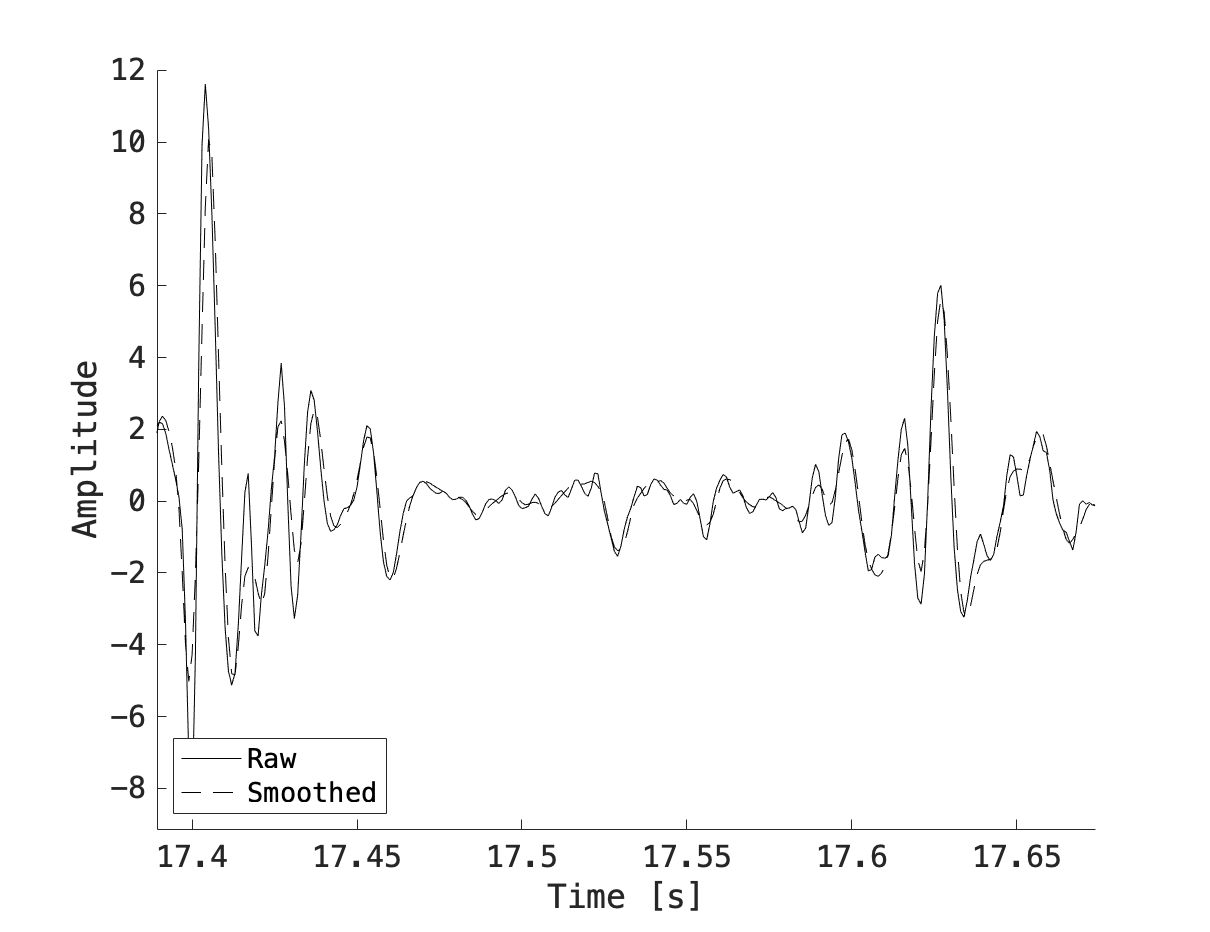
\includegraphics[scale=0.3]{sections/chapter-07/images/pcg-example.png}
    \caption[Segmento del fonocardiograma de un paciente sano]{Segmento del fonocardiograma de un paciente sano. En línea sólida se muestra la entrada sin ningún tipo de acondicionamiento y en línea punteada la señal suavizada.}
    \label{fig:springer-pcg-example}
\end{figure}

\section{Extracción de marcas} \label{sec:annotations}

\indent El etiquetamiento de los fonocardiogramas de entrenamiento necesitan de las anotaciones de la onda R y del fin de la onda T. Esto fue propuesto por Schmidt \textit{et al.} en \cite{pp:schmidt2010}, donde propone que los sonidos fundamentales del fonocardiograma, S$_1$ y S$_2$ tienen una media y un desvío asociado. Simplemente midió la duración de S$_1$ y S$_2$ para luego calcular la media y el desvío muestral, concluyendo que la duración se mantiene relativamente constante siendo de ($122 \pm 32$) ms y ($92 \pm 28$) ms con un $95\%$ de intervalo de confianza. \\
\indent Para la extracción de marcas del \acrshort{ecg}, éstas fueron hechas automáticamente por algoritmos de delineación. Para ello se compararon 4 detectores para la detección de la onda R y el fin de la onda T. El hecho de que haya ruido y artefactos en el \acrshort{ecg} provocará que las anotaciones de los detectores no coincidan. Para ello, para asegurar que las anotaciones sean de calidad, se derivó un \textit{Signal Quality Index} (SQI) mediante la concordancia entre los detectores. \\
\indent Los detectores utilizados para la detección de la onda R fueron gQRS, jQRS (anteriormente utilizados en \cite{ref:behar} y \cite{ref:behar-oster-clifford}), el algoritmo basado en lo que se conoce como \textit{Parabolic fitting} utilizado en \cite{ref:illanes-zhang} y el delineador de onditas. Ahora para la detección del fin de la onda T se utilizó el algoritmo conocido como \textit{ecgpuwave} (basado en la detección previa del complejo QRS), un método basado en maximizar el área de una ventana móvil entre sucesivas ondas R \cite{ref:zhang}, el delineador de onditas y un algoritmo hecho por Vazquez-Seisdedos et al. \cite{ref:seisdedos}. Para decir que los detectores son consistentes entre si las anotaciones no deben estar más alejadas que 100 ms.

\begin{figure}[H]
    \centering
    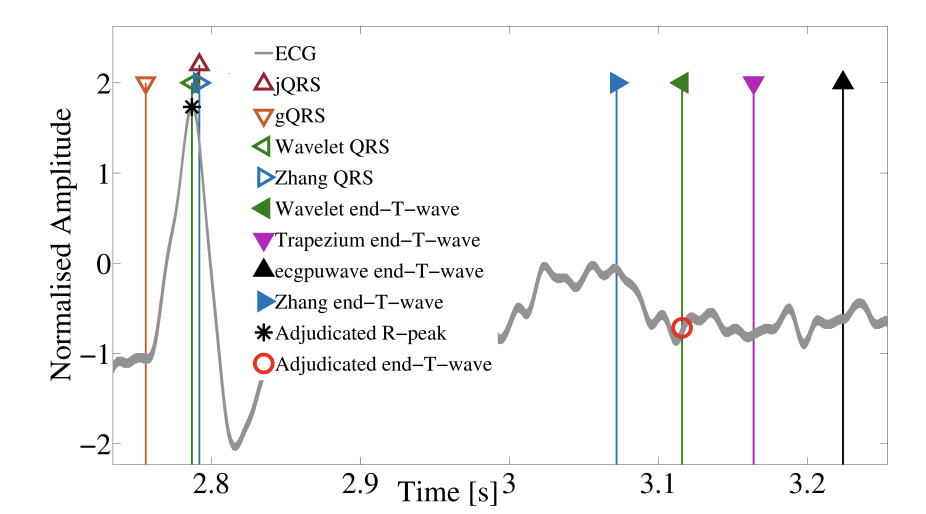
\includegraphics[scale=0.8]{sections/chapter-04/images/detector-agreement.png}
    \caption[Ejemplo de las anotaciones de una señal de \acrshort{ecg} con ruido. La posición de las anotaciones para cada uno de los detectores se muestran]{Ejemplo de las anotaciones de una señal de \acrshort{ecg} con ruido. La posición de las anotaciones para cada uno de los detectores se muestran. Imagen extraída de \cite{pp:springer2015}.}
    \label{fig:detector-agreement}
\end{figure}

\section{Etiquetamiento}

\indent El etiquetamiento (\textit{labeling}), corresponde a obtener etiquetas realizadas de forma manual o automática generalmente utilizadas en el entrenamiento del modelo propuesto. Este método es lo que se conoce como \textit{aprendizaje supervisado}, donde se necesita tener catalogada la entrada para estimar los parámetros del modelo. \\
\indent El etiquetamiento, como se ha explicado en el Sección \ref{sec:annotations}, consiste en estimar los tiempos de duración de los sonidos. Sin embargo, para el conjunto de datos de este trabajo, las estimaciones de Schmidt \textit{et. al} no dieron buenos resultados, dado a que en el momento del etiquetamiento los estados no quedaban bien definidos. Para ello, se modificaron las medias a ($122 \pm 22$) ms y ($152 \pm 22$) ms. Es necesario mencionar que el algoritmo propuesto por Springer \textit{et. al} sea, tal vez, el responsable de la necesidad de adaptar los parámetros de manera ad hoc. \\
\indent En la Figura \ref{fig:pcg-labeling} se observa una porción de una señal de \acrshort{pcg} donde, en base a las marcas proveídas por la base de datos, se realiza el etiquetado de los estados de la señal [sístole (S$_1$), sístole isovolumético, diástole (S$_2$), diástole isovolumétrico].

\begin{figure}[H]
    \centering
    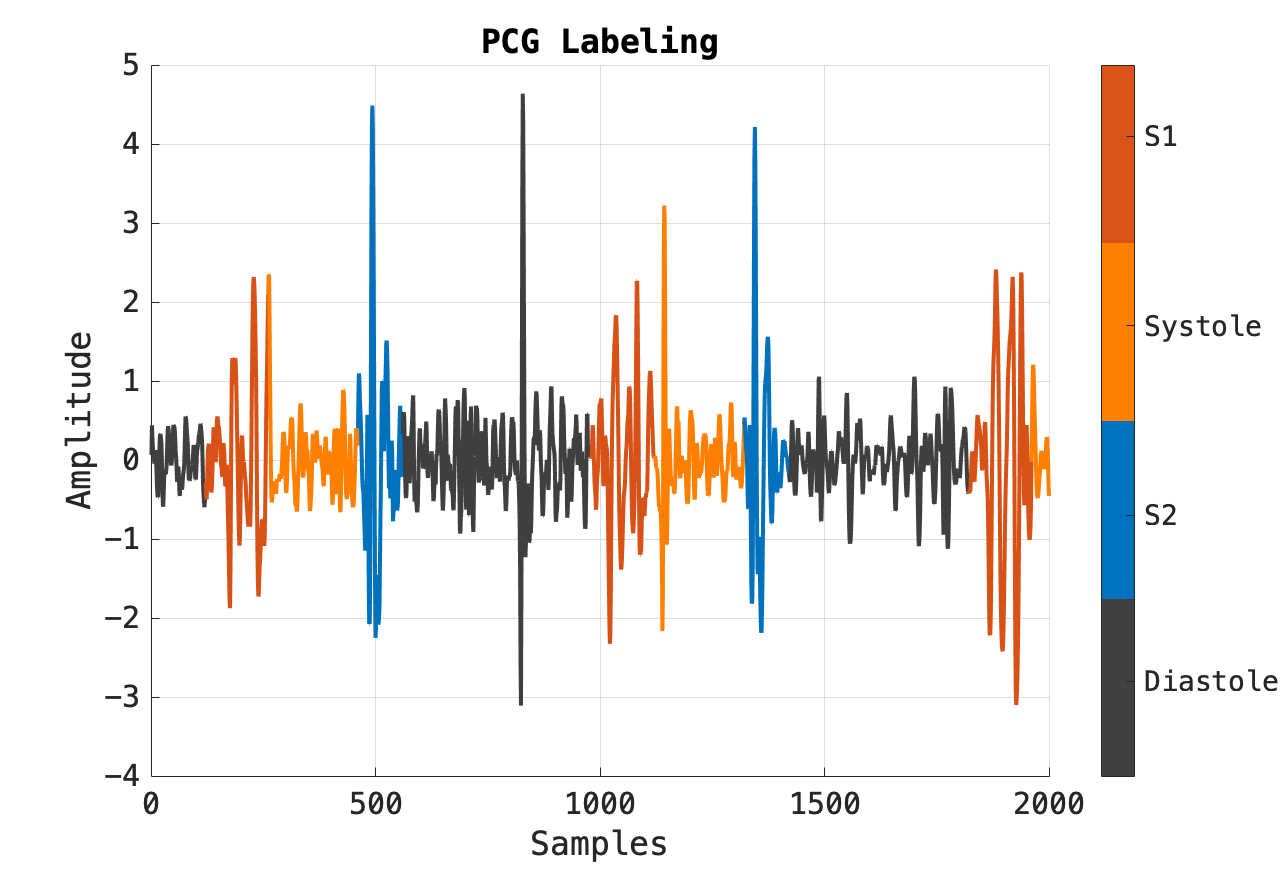
\includegraphics[scale=0.3]{sections/chapter-04/images/pcg-labeling.png}
    \caption[Segmento de una señal de fonocardiograma etiquetada]{Segmento de una señal de fonocardiograma etiquetada. En color rojo se marcan los sonidos S$_1$, en naranja el sístole isovolumétrico, en azul los sonidos S$_2$ y en negro el diástole isovolumétrico.}
    \label{fig:pcg-labeling} 
\end{figure}

\subsection*{Algoritmo etiquetador}

\indent Sea una señal envolvente del fonocardiograma $\bm{x}_i \in \mathbb{R}^{N_i}$ y las posiciones de las marcas del electrocardiograma asociadas $\bm{r}_i \in \mathbb{R}^{M_i}$, $\mathbf{t}_i \in \mathbb{R}^{M_i}$. Se definen las medias y desvíos de los sonidos, ($\mu_{S_1}, \sigma_{S_1}$) y ($\mu_{S_2}, \sigma_{S_2}$). \bigskip

\indent Se define $\mathbf{s}_i \in \mathbb{R}^{N_i}$ al vector de estados de la señal. Recordar que este vector sólo puede tomar 4 valores, $\mathbf{s}_i \in [1,4]$. \\
\indent A partir de aquí se mencionara el algoritmo para etiquetar cada uno de los cuatro estados.

\subsubsection*{Primer sonido (Estado \#1)}

\indent Para el marcado del primer sonido o estado, se define un umbral superior en base a la posición de la onda R. 

\begin{align}
    U_{b,i} = \left[\mathrm{min}(N_i,\mathbf{r}_i+\mu_{S_1})\right] 
\end{align}

\indent Donde $[x]$ es el entero más cercano a $x$.

\begin{align}
    \bm{s}_j = \mathds{1}\left\{\mathrm{max}(1, \mathbf{r}_i) < j < \mathrm{min}(U_{b,i}, N_i)\right\}
\end{align}

\subsubsection*{Segundo sonido (Estado \#3)}

\indent Para el etiquetado del segundo sonido o tercer estado, se requiere definir una ventana de búsqueda como así también dos umbrales, uno inferior y otro superior. \\
\indent Los umbrales se definen de la siguiente manera y dependen de cada una de los finales de las ondas T.

\begin{align}
    U_{b,i} = \mathrm{min}(N_i,\lceil t_i+\lfloor \mu_{S_2} + \sigma_{S_2} \rfloor \rceil)
\end{align}

\begin{align}
    L_{b,i} = \mathrm{max}(t_i-\lfloor \mu_{S_2} + \sigma_{S_2} \rfloor,1)
\end{align}

\indent Se define los enteros superiores e inferiores según la siguiente notación.

\begin{align*}
    \lceil x \rceil := \mathrm{sup}\big\{n \; | \; n \in \mathbb{Z}, \hspace{2mm} x \leq n\big\} \\
    \lfloor x \rfloor := \mathrm{inf}\big\{n \; | \; n \in \mathbb{Z}, \hspace{2mm} x \geq n\big\}
\end{align*}

\indent Luego, se define la ventana de búsqueda en la ecuación \ref{eq:search-window}. Para cada posición del final de la onda T se define una ventana. En ella se busca el índice del máximo valor.

\begin{align}
    \label{eq:search-window}
    \bm{\Tilde{s}}_{w,i} = \prod_{k=L_{b,i}}^{U_{b,i}} \bm{x}_k \cdot \mathds{1}\big\{\mathbf{s}_k \neq 1\big\}
\end{align}

\begin{align}
    l_i = \arg \underset{j \in [L_{b,i},U_{b,i}]}{\mathrm{max}} \Big(\bm{\Tilde{s}}_{w,i}\Big)
\end{align}

\indent Una vez extraído la posición del máximo, es necesario calcular el centro de la ventana.

\begin{align}
    c_{w,i} = \mathrm{min}\Big(N_i,l_i+L_{b,i}\Big)
\end{align}

\subsubsection*{Diástole isovolumétrico (Estado \#4)}

\indent De esta manera es posible calcular las muestras que corresponden al tercer estado. Antes es necesario redefinir el umbral superior.

\begin{align}
    U_{b,i} = \mathrm{min}\left(N_i, \left\lceil  c_{w,i} + \frac{1}{2}\mu_{S_2} \right\rceil \right)
\end{align}

\begin{align}
    \mathbf{s}_j = 3 \cdot \mathds{1}\left\{\mathrm{max}\left(\lceil c_{w,i}-\frac{1}{2}\mu_{S_2}\rceil, 1\right) < j < U_{b,i}\right\}
\end{align}

\indent Con $j=0,1,2,\dots,M-1$. \bigskip

 \indent Una vez definidos los estados 1 y 3, correspondientes a S$_1$ y S$_2$ respectivamente, es posible definir el cuarto estado. \\
\indent Es necesario obtener la diferencia entre todos las posiciones de la onda R y la onda T. Para ello se define el vector $\mathbf{d}_i \in \mathbb{R}^M$, donde sus componentes son $d_{j,i}$, con $i = 0,1,2,\dots,M-1$ y $j = 0,1,2,\dots,M-1$. 

\begin{align}
    d_{j,i} = \begin{cases}
                \infty, \qquad &r_j - t_i < 0 \\
                r_j - t_i, \quad &\mathrm{otro \; caso}
              \end{cases}
\end{align}


\begin{align}
    p_i = \begin{cases}
            N, \quad &\sum_{j=1}^{M_i} \mathds{1}\big\{d_{j,i} < \infty\big\} =  0  \\
            t_{\arg \underset{j}{\mathrm{min}} \; \mathbf{d}_i} -1, \quad  & \mathrm{otro \; caso}
          \end{cases}
\end{align}

\begin{align}
    \mathbf{s}_j = 4 \cdot \mathds{1}\left\{\left\lceil c_{w,i} + \frac{1}{2}(\mu_{S_2} + \sigma_{S_2}) \right\rceil < j < p_i  \right\}
\end{align}

\subsubsection*{Inicio y fin de la señal}

\indent Dado a que todos los estados derivan de la posición de la onda R y del fin de la onda T, el primer estado en la señal siempre será 1 o 3. Por lo tanto, hasta ese estado, debe ser 2 o 4 respectivamente. 

\indent Tanto para el inicio como el fin de la señal es necesario obtener desde izquierda a derecha la posición del primer estado y el último estado en $\mathbf{s}$. Las ecuaciones \ref{eq:min-index}, \ref{eq:max-index} reflejan como calcular dichos índices.

\begin{align} \label{eq:min-index}
    f_n = \mathrm{min}\big\{ n \in \mathbb{N}_0, \; | \; s_n \neq 0  \big\}
\end{align}

\begin{align} \label{eq:max-index}
    l_n = \mathrm{max}\big\{ n \in \mathbb{N}_0, \; | \; s_n \neq 0  \big\}
\end{align}

\indent Luego, se definen los estados del inicio y del final de la señal.

\begin{align}
    s_j = \begin{cases}
        2, \quad s_{f_n} = 3  \\
        4, \quad s_{f_n} = 1
        \end{cases}, \quad \mathrm{con} \; j = 0,1,\dots,f_n-1
\end{align}

\begin{align}
    s_j = \begin{cases}
        2, \quad s_{l_n} = 1  \\
        4, \quad s_{l_n} = 3
        \end{cases}, \quad \mathrm{con} \; j = l_n+1,l_n+2,\dots,M-1
\end{align}

\subsubsection*{Sístole isvolumétrico (Estado \#2)}

\indent Todos los estados las muestras que no han sido definidos son las correspondientes al estado 2.

\begin{align}
    s_j = \begin{cases}
        2, \quad s_j = 0  \\
        s_j, \quad s_j \neq 0
        \end{cases}, \quad \mathrm{con} \; j = 0,1,\dots,M-1
\end{align}



  \chapter{Procesamiento}

\section{Identificación y construcción de características}

\indent Generalmente para la detección o clasificación se utiliza lo que se conoce como atributos
(\textit{features}). Estos atributos son necesarios para realizar estimaciones de todo tipo, desde casos sencillos
para la estimación de la altura y peso promedio en una población hasta detección de obstáculos para los algoritmos
de evasión. En este caso particular, para estimar dónde comienzan y finalizan los estados de un \acrshort{pcg}, es
necesario también contar con atributos que ayuden a los algoritmos de segmentación a definir éstos. \\
\indent En el caso de señales en el tiempo o \textit{time-series} existen distintos tipos de atributos que se pueden
extraer. Ejemplos de estos son, amplitud, energía, contenido espectral, entre otros. Por supuesto, que no siempre
todos los atributos de la señal son aptos para el tipo de estimación que se desea efectuar. \\
\indent Los enfoques de clasificación de sequencias que se abordan aquí son: 1) sequencia a sequencia
(\textit{sequence-to-sequence}), 2) secuencia a etiqueta (\textit{sequence-to-label}). La primera implica que la
longitud de la entrada sea conocida, fija e igual que la salida del bloque de clasificación o segmentación y la
segunda implica sólo tener una etiqueta de lo que la entrada representa. Los casos que se manejan en este trabajo
son las técnicas de clasificación de señales sanas y patológicas. El caso más sencillo las etiquetas son dos: 1)
sano, 2) patológico y las técnicas de segmentación en las cuales se basa el presente trabajo, donde se quiere
etiquetar o segmentar la secuencia de entrada (esto significa ponerle un valor a cada muestra de la secuencia en el
tiempo).

\subsection*{Características base}

\indent Una importante etapa en el proceso comienza con la extracción de atributos propuestos por David Springer
\textit{et al.} \cite{pp:springer2015} A continuación se listan algunos atributos: \\
\indent 1) Envelograma homomórfico (\textit{homomorphic envelogram}): Este procedimiento es muy similar a la
modulación AM. Esta técnica ha sido usada por numerosos investigadores para la extracción de envolventes del
\acrshort{pcg} \cite{ref:gupta}, \cite{ref:gill-gavrieli-intrator}, incluido el algoritmo de segmentación
\cite{pp:schmidt2010}. El envelograma homomórfico es derivado de aplicarle el logaritmo natural a la señal en
cuestión $x(n)$. Esta señal se la modela como la multiplicación de una señal de baja frecuencia envolvente y una
oscilación de más alta frecuencia.

\begin{equation}
  x(n) = a(n) \cdot o(n)
\end{equation}

El logaritmo natural aplicado a esto implica que se pueda separar en una suma ambas componentes.

\begin{equation}
  \ln(x(n)) = \ln(a(n)) + \ln(o(n))
\end{equation}

De esta manera con un filtro pasa-bajos, con una frecuencia de corte adecuada, se logra filtrar las osilaciones $o
(n)$ y se obtiene $a(n)$ con la ecuación \ref{eq:henv-eq}.

\begin{align} \label{eq:henv-eq}
a(n) = \exp(\mathcal{H}(\ln(x(n)))
\end{align}

Donde el operador $\mathcal{H}$ es el filtro pasa-bajos.

\begin{align*}
  a(n) &= \exp(\mathcal{H}(\ln(a(n)) + \ln(o(n))) \\
  a(n) &= \exp(\ln(a(n)))
\end{align*}

\indent 2) Envolvente de Hilbert (\textit{Hilbert envelope}): Messer et al. \cite{ref:messer} y
Kumar et al. \cite{ref:kumar} calcularon la envolvente del \acrshort{pcg} usando la transformada de Hilbert.
La transformada de Hilbert extrae la función analítica que excluye las frecuencias negativas de la señal original
y su envolvente se obtiene calculando el módulo. \\
\indent 2) Envolvente de onditas (\textit{wavelet envelope}): el análisis de onditas ha sido ampliamente explorado.
Sin embargo, hay discusiones sobre cuál familia es la óptima para el filtrado, clasificación y segmentación del
\acrshort{pcg}. Algunos investigadores determinan que la familia Morlet es la que mejor concuerda en el análisis de
fonocardiogramas \cite{ref:oskiper-watrous,ref:ergen-tatar-gulcur}.
Otros destacan la familia de Daubechies \cite{ref:liang-sakari-iiro,ref:gupta}.
En este caso se ha utilizado la \acrshort{dwt} con distintas familias y niveles (la familia de Morlet no ha sido
utilizada dado que \acrshort{dwt} no es compatible con esta familia). \\
\indent 3) Envolvente de densidad espectral de potencia (\textit{power spectral density envelope}): la mayoría del
contenido espectral de S$_1$ y S$_2$ se encuentra por debajo de 150 Hz con un pico en 50 Hz. Basado en estas
frecuencias, se extrae este atributo entre 40 Hz y 60 Hz, en ventanas con 50\% de solapamiento y ancho de 0.05 s.
La PSD fue calculada utilizando ventaneo de Hamming y transformada de Fourier. \\
\indent Cada uno de los 4 atributos extraídos se los normaliza en varianza y media.
Luego, se realiza un submuestreo a 50 Hz por motivos computacionales.

\subsection*{Transformada sincronizada de Fourier}

El análsis frecuencio-temporal y de escala de tiempo son herramientas estándar para el estudio de señales no
estacionarias o determinísticas con variación frecuencial. En particular, señales multicomponentes, por ejemplo
superposición de amplitud y ondas moduladas en frecuencia (\acrshort{am}-\acrshort{fm}), son bien analizadas con la
Transformada de tiempo corto de Fourier (\acrshort{fsst}) \cite{ref:gabor} y la Transformada Continua de Onditas
(\acrshort{cwt}) \cite{ref:grossmann-morlet}. Es bien conocido que ambas transformadas para estas señales dibujan
una especie de líneas en los planos de \acrshort{tf} (tiempo-frecuencia) o \acrshort{ts} (escala de tiempo),
alrededor de crestas que corresponden a la frecuencia instantánea de los modos que hacen a la señal. \\
\indent La \acrshort{sst} (Tranformada sincronizada), introducida en \cite{ref:daubechies-maes}, es una suerte de
reasignación al método que trata de ajustar la representación TS manteniendo la invertibilidad. Esta técnica se
desarrolló en el contexto de la \acrshort{cwt} pero sin ningún tipo de avances en el campo de la \acrshort{stft}.

\subsection*{Transformada de tiempo corto de Fourier y señales multicomponentes}

\indent Denotamos la transformada de Fourier con la siguiente notación $\hat{f}(\eta)$ para la función $f(t)$.

\begin{equation}
  \hat{f}(\eta) = \int_{-\infty}^\infty f(t)e^{-2i\pi\eta t}dt
\end{equation}

\indent La \acrshort{stft} es una versión local de la transformada de Fourier obtenida por medio de una ventana
deslizante $g$:

\begin{equation}
  V_f(\eta,t) = \int_{-\infty}^\infty f(\tau)g(t-\tau)e^{-2i\pi\eta (t-\tau)}d\tau
\end{equation}

\indent La representación de $|V_f(\eta,t)|^2$ en el plano TF es lo que se conoce como \textit{espectrograma} de la
señal $f$. \\
\indent De esta manera, se analiza señales multicomponentes AM-FM con la \acrshort{stft}.

\begin{equation}
  f(t) = \sum_{k=1}^K f_k(t) = \sum_{k=1}^K A_k(t) e^{2i\pi\phi_k(t)}
\end{equation}

\indent Si se asume que las variaciones en amplitud y frecuencia son lentas, se puede escribir la siguiente
aproximación alrededor de un tiempo fijo $t_0$, lo cual equivale a aproximar $f$ por funciones puras.

\begin{equation}
  f(t) \approx \sum_{k=1}^K A_k(t_0) e^{2i\pi[\phi_k(t_0)+\phi_k^{'}(t_0)(t-t_0)]}
\end{equation}

\indent La correspondiente \acrshort{stft} aproximada se escribe (cambiando $t_0$ por un $t$ genérico).

\begin{equation}
  V_f(\eta,t) \approx \sum_{k=1}^K f_k(t) \Tilde{g}(\eta-\phi_k^{'}(t))
\end{equation}

\indent Esto muestra que la representación de una señal multicomponente en el plano TF se encuentra concentrada
alrededor de crestas definidas por $\eta=\phi_k^{'}(t)$. Si las frecuencias $\phi_k^{'}$ se encuentran lo
suficientemente separadas cuando $k$ varía, cada modo ocupa un dominio distinto del plano TF, permitiendo la
detección, separación y reconstrucción.

\subsection*{Sincronización basada en Fourier}

\indent El objetivo de la \acrshort{sst} tiene dos aspectos: proveer una representación concentrada de señales
multicomponentes en el plano TF, y una descomposición que permite separar y demodular los diferentes modos.

\subsubsection*{Motivación-definición}

\indent A partir de la \acrshort{stft} $V_f$, la \acrshort{fsst} mueve los coeficientes $V_f(\eta,t)$ según la
transformación $(\eta,t) \rightarrow (\hat{\omega}_f(\eta,t),t)$ donde $\hat{\omega}_f$ es la \textit{frecuencia
instantánea} definida por:

\begin{align}
  \hat{\omega}_f(\eta,t) = \frac{1}{2\pi} \partial_t \arg V_f(\eta,t) = \mathcal{R}e\left(\frac{1}{2\pi
  i}\frac{\partial_t V_t(\eta,t)}{V_f(\eta,t)}\right)
\end{align}

\indent Este operador es simplemente la frecuencia instantánea de la señal a un dado tiempo $t$, filtrada en la
frecuencia $\eta$. Esto es una buena aproximación local de la frecuencia instantánea $\phi_k^{'}(t)$. El segundo
punto importante de la \acrshort{sst} es la reconstrucción "vertical", que se encuentra en $L^2(\mathbb{R})$ siendo
la ventana $g$ continua y distinta de cero en $t=0$.

\begin{align} \label{eq:vertical_reconstruction}
  f(t) = \frac{1}{g(0)} \int_{-\infty}^\infty V_f(\eta,t)d\eta
\end{align}

\indent Ésto permite definir la \acrshort{fsst}, lo cual consiste en restringir el dominio de integración de
[\ref{eq:vertical_reconstruction}] al intervalo donde $\hat{\omega}_f(\eta,t) = \omega$, escribiendo:

\begin{align}
  T_f(\omega,t) = \frac{1}{g(0)} \int_{-\infty}^\infty V_f(\eta,t)\delta(\omega-\hat{\omega}_f(\eta,t))d\eta
\end{align}

\indent A continuación se muestra la comparación entre una \acrshort{stft} y una \acrshort{fsst}. El ejemplo
consiste en una señal con dos componentes frecuenciales, dado $\Omega_0=\frac{2}{5}\pi$. La señal $x(n)$ se describe
en la ecuación \ref{eq:i_e_signal}

\begin{align} \label{eq:i_e_signal}
  x(n) = \sin(\Omega_0 n) + 3\sin(2\Omega_0 n), \; n \in [0,1023]
\end{align}

\begin{figure}[H]
\centering
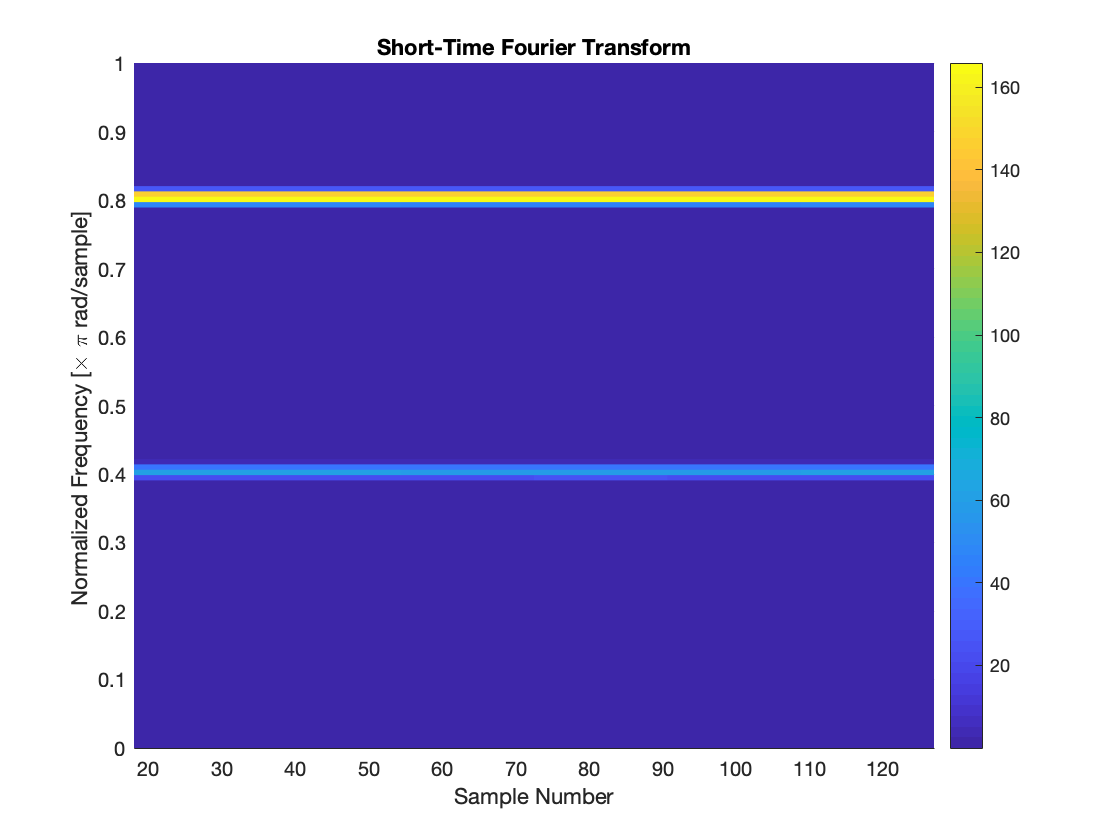
\includegraphics[scale=0.35]{chapters/chapter-05/images/stft.png}
\caption[Espectrograma de una señal sinusoidal de dos tonos]{Espectrograma de una señal sinusoidal de dos tonos.
Generación de una señal suma de dos sinusoidales de 1024 muestras con ruido blanco Gaussiano. La frecuencia más alta
presenta una amplitud mayor que la de baja frecuencia.}
\label{fig:i_e_stft}
\end{figure}

\begin{figure}[H]
  \centering
  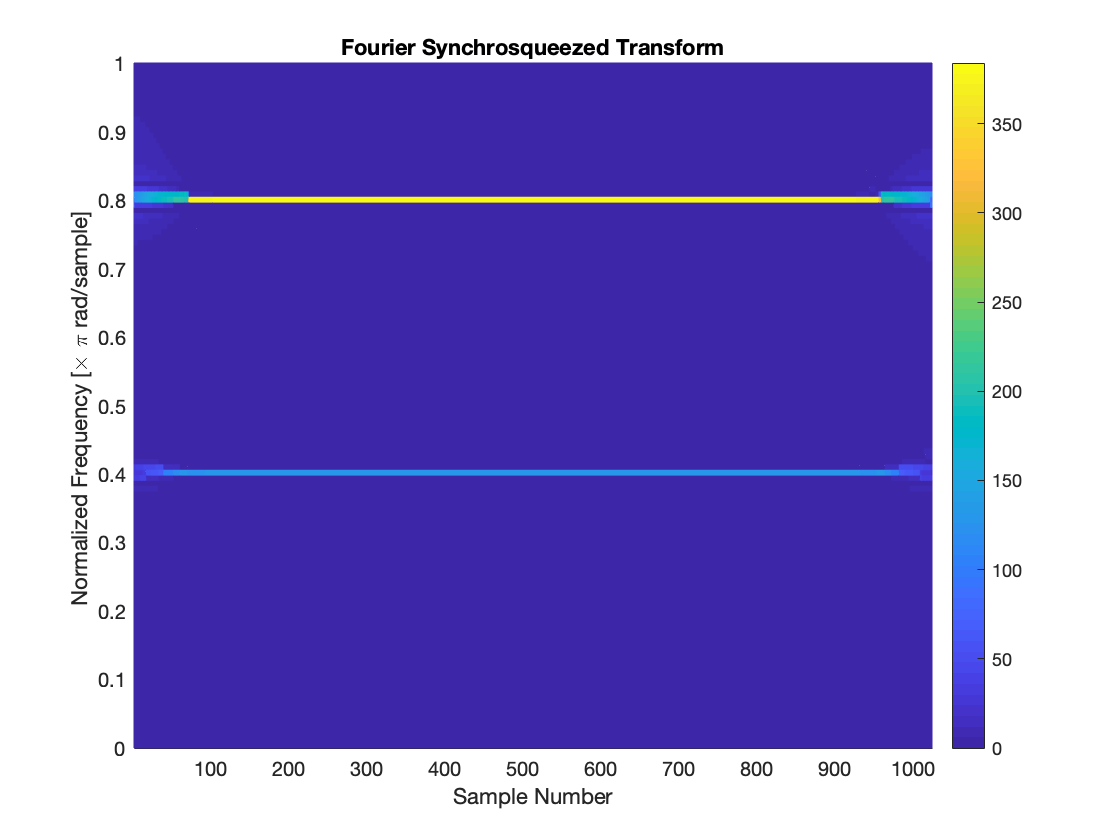
\includegraphics[scale=0.35]{chapters/chapter-05/images/fsst.png}
  \caption[\acrshort{fsst} de una señal sinusoidal de dos tonos]{\acrshort{fsst} de una señal sinusoidal de dos tonos.
  Generación de una señal suma de dos sinusoidales de 1024 muestras con ruido blanco Gaussiano. La frecuencia más alta
  presenta una amplitud mayor que la de baja frecuencia.}
  \label{fig:i_e_fsst}
\end{figure}

\indent Observando ambas Figuras \ref{fig:i_e_stft} y \ref{fig:i_e_fsst} se nota a simple vista la concentración de
energía de ambos tonos en la \acrshort{fsst}, mientras que en la \acrshort{stft} no. Esto deja evidenciado en la
implementación el concepto de crestas mencionado anteriormente.

  \chapter{Deep learning} \label{ch:deep-learning}

\indent \textit{Deep Learning} es un conjunto de métodos de aprendizaje que intentan modelar problemas con
arquitecturas complejas combinando diferentes transformaciones no lineales. Los pilares fundamentales son las redes
neuronales. Combinadas logran formar las \acrshort{dnn} (\textit{deep learning neural network}).
\indent Estas técnicas han logrado un avance significativo en los campos de procesamiento de sonidos y de imágenes,
éstos incluyen reconocimiento facial, reconocimiento del habla, visión computadorizada, entre otros.

\section{Redes neuronales}

\indent Una red neuronal artificial es una aplicación, no lineal respecto a su parámetros $\theta$ asociado a una
entrada $x$ y una salida $y = f(x,\theta)$. Por simplificación $y \in \mathbb{R}$ pero puede ser que $y$ sea
multidimensional, $\textbf{y} \in \mathbb{R}^n$. La red neuronal puede ser utilizada para regresión o clasificación.
En aprendizaje estadístico, como es usual, se estima un parámetros $\theta$ a partir de una muestra. Generalmente,
la función a minimizar no es convexa y resulta en minimizaciones locales. Existe un método muy eficiente para
computar el gradiente de una red neuronal. Éste llamado retropropagación del gradiente (\textit{backpropagation of
the gradient}), permite obtener una minimización local de un criterio cuadrático fácilmente.

\section{Perceptrón}

\indent Un perceptrón es una función $f_j$ de la entrada $\mathbf{x} = (x_1, ...,x_d)$ pesado por un vector
$\mathbf{w} = (w_{j,1}, ..., w_{j,d})$, completado por un sesgo $b_j$ y asociado a una función de activación $\phi$.

\begin{align}
  y_j = f_j(x) = \phi(<w_j,x>) + b_j
\end{align}

\subsection*{Funciones de activación}

\begin{itemize}
  \item Función de identidad:
  \begin{align}
    \phi(x) = x, \; -\infty < x < \infty
  \end{align}

  \item Función sigmoidea:
  \begin{align}
    \phi(x) = \frac{1}{1+e^{-x}}, \; -\infty < x < \infty
  \end{align}

  \item Función tangente hiperbólica:
  \begin{align}
    \phi(x) = \frac{e^{x}-e^{-x}}{e^{x}+e^{-x}} = \frac{e^{2x}-1}{e^{2x}+1}, \; -\infty < x < \infty
  \end{align}

  \item Función de umbral (\textit{hard-threshold}):
  \begin{align}
    \phi(x) = \mathbf{1}_{x \geq \beta}, \; -\infty < x < \infty
  \end{align}

  \item Función rectificadora lineal (\textit{rectified linear unit}):
  \begin{align}
    \phi(x) = \max(0,x), \; -\infty < x < \infty
  \end{align}
\end{itemize}

\indent En la Figura \ref{fig:neuron-schematic} se ilustra un esquemático de una neurona donde $\Sigma = <w_j,x> + b_j$.

\begin{figure}[H]
  \centering
  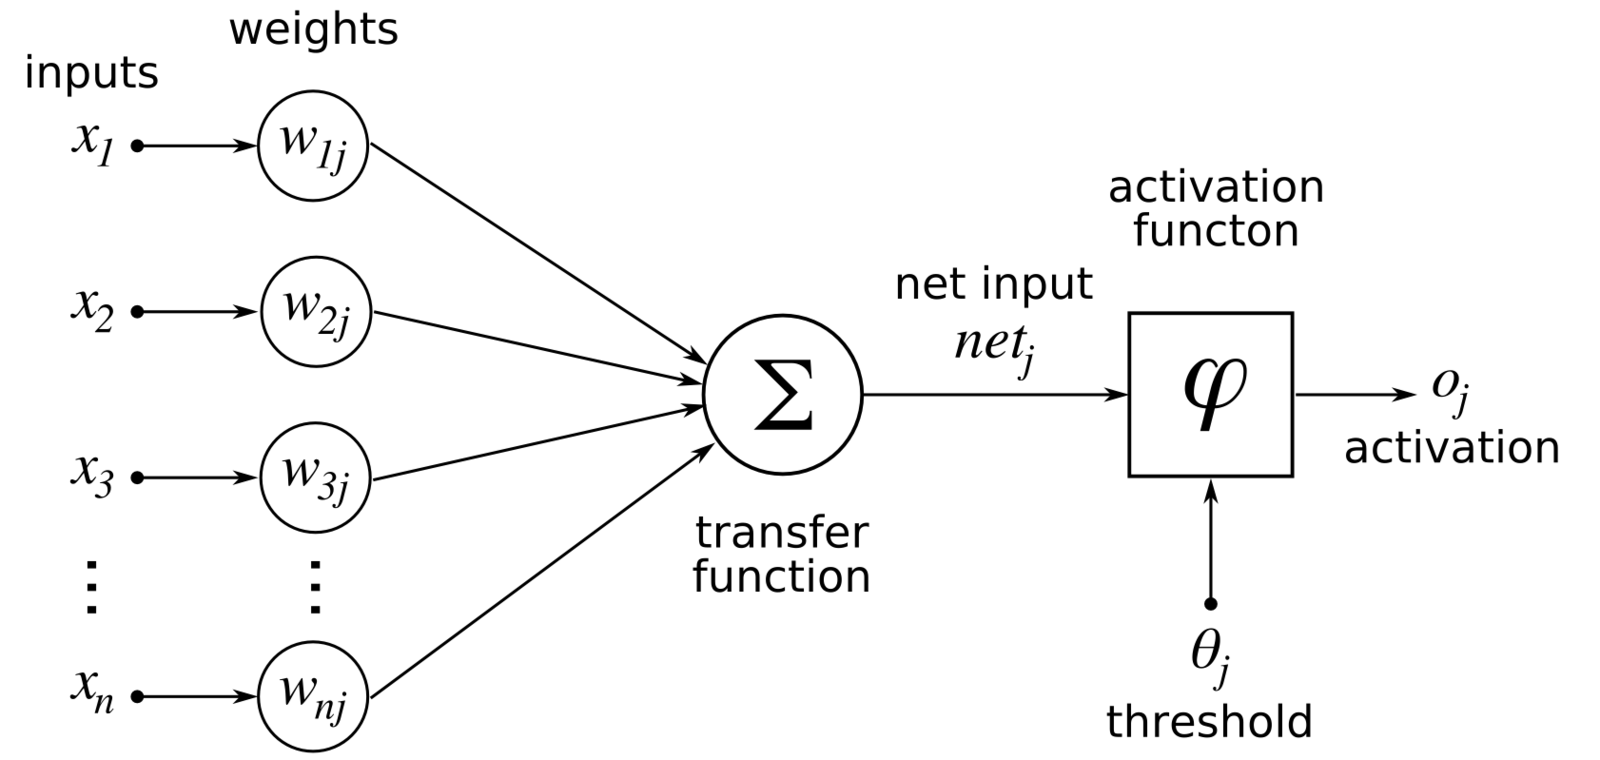
\includegraphics[scale=0.2]{sections/chapter-06/images/neuron-schematic.png}
  \caption[Esquemático de una neurona]{Esquemático de una neurona. Imagen obtenida de \href{https://commons
  .wikimedia.org/wiki/File:ArtificialNeuronModel_english.png}{Wikimedia Commons}.}
  \label{fig:neuron-schematic}
\end{figure}

\indent Históricamente, la función sigmoidea fue mayormente utilizada ya que es diferenciable y permite mantener los
valores entre [0,1]. Sin embargo, es problemática ya que su gradiente es muy cercano a cero cuando $|x|$ no es se
encuentra cerca de 0.

\begin{figure}[H]
  \centering
  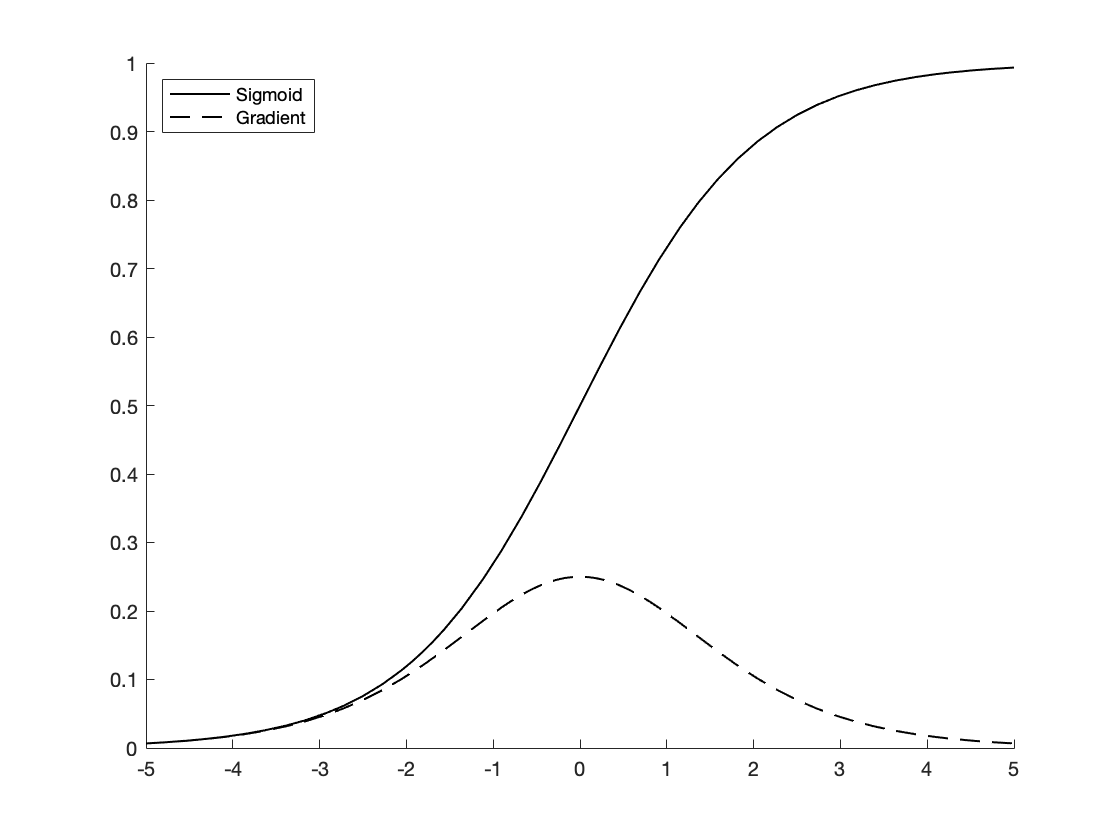
\includegraphics[scale=0.3]{sections/chapter-06/images/sigmoid.png}
  \caption[Función de activación sigmoidea.]{Función de activación sigmoidea. El línea sólida se muestra la función
  de activación y su derivada en línea punteada.}
  \label{fig:relu}
\end{figure}

\indent Es el caso de \textit{deep learning} que se utilizan múltiples capas de redes neuronales, lo cual trae
problemas
con el algoritmo de retropropagación para estimar parámetros. Éste es el por qué la función sigmoidea fue reemplazada
por la función \acrshort{relu} (\textit{Rectified Linear Unit}).

\begin{figure}[H]
  \centering
  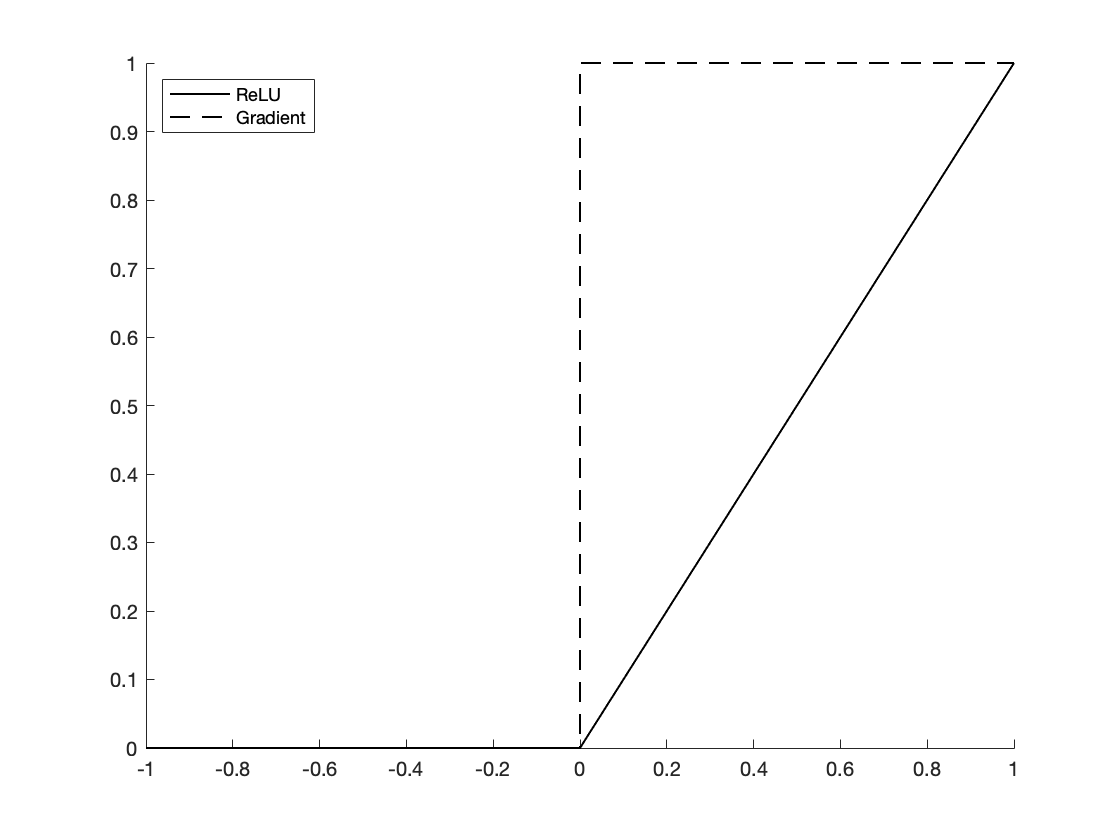
\includegraphics[scale=0.3]{sections/chapter-06/images/ReLU.png}
  \caption[Función de activación \acrshort{relu}.]{Función de activación \acrshort{relu}. El línea sólida se muestra
  la función de activación y su derivada en línea punteada.}
  \label{fig:sigmoid}
\end{figure}

\indent Esta función no es diferenciable en cero, pero en la práctica esto no es un problema dado a que la
probabilidad de que una entrada sea igual a cero es casi nula. La función \acrshort{relu} también tiene la propiedad
de dispersión (\textit{sparcification}). Ella y su derivada son 0 para valores negativos, y no es posible obtener
información en estos casos, pero eso es recomendable agregar un pequeño sesgo para asegurar de que cada unidadad se
encuentre activa. Muchas variaciones de la función \acrshort{relu} consideran mantener a las unidades siempre
activas y que sus gradientes para valores negativos no sean 0.

\section{Perceptrón multicapa}

\indent Un perceptrón multicapa (o una red neuronal) es una estructura compuesta por varias capas, las cuales en la
literatura se las denomina capas ocultas (\textit{hidden layers}), compuestas por neuronas donde su salida son la
entrada de las neuronas de la siguiente capa. Más aún, la salida de una neurona puede ser la entrada de otra neurona
de la misma o anterior capa (es el caso de las redes neuronales recurrentes). En la última capa, denominada capa de
salida, es posible aplicar una función de activación distinta a las aplicadas en las capas intermedias dependiendo
del problema en cuestión: regresión o clasificación.

\begin{figure}[H]
  \centering
  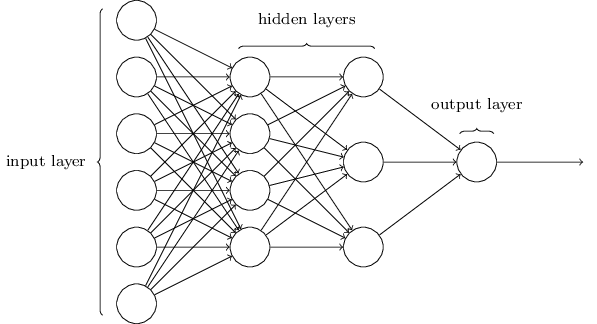
\includegraphics[scale=0.6]{sections/chapter-06/images/mlp-network.png}
  \caption[Perceptrón multicapa]{Perceptrón multicapa. Imagen obtenida del \href{https://github
  .com/rcassani/mlp-example}{repositorio de Raymundo Cassani}}
  \label{fig:mlp_net}
\end{figure}

\indent \acrshort{mlp} (Multilayer perceptron) tienen una arquitectura básica. Cada unidad o neurona de una capa se
conecta a todas las neuronas de la siguiente capa y no tienen conexión con las neuronas de la misma capa. Los
parámetros de la arquitectura son la cantidad de capas y el número de unidades por capa. Generalmente, como se ha
dicho antes, la función de activación es diferente a las otras intermedias. En el caso de clasificación binaria, la
salida genera una predicción de $\mathbb{P}(Y=1|X)$ ya que ese valor es [0,1], y la función de activación sigmoidea
es utilizada. Para un caso de clasificación multiclase (N es la cantidad de clases), la capa de salida se compone de
N neuronas, generando una predicción de $\mathbb{P}(Y=i|X)$, siendo $i=1,2,...,N$. Por supuesto, al ser
probabilidades, la suma de todas éstas deben sumar 1. \\
\indent La mayoría de las veces se usa la función multidimensional \textit{softmax}.

\begin{align}
  \mathrm{softmax}(z)_i = \frac{e^{z_i}}{\sum_j e^{z_j}}
\end{align}

\indent La formulación matemática para el perceptrón multicapa se define con $L$ capas intermedias.

\begin{enumerate}
  \item La capa de entrada (\textit{input layer}) se define para $k=0$.

  \begin{align*}
    h^{(0)}(\bm{x}) = \bm{x}
  \end{align*}

  \item Para las capas ocultas se define $k = 1,2,...,L$.

  \begin{align*}
    a^{(k)}(\bm{x}) &= \bm{b}^{(\bm{x})} + \mathbf{W}^{(k)}h^{(k-1)}(\mathbf{x}) \\
    h^{(k)}(\bm{x}) &= \phi(a^{(k)}(\bm{x}))
  \end{align*}

  \item Para $k = L+1$, la capa de salida (\textit{output layer}).

  \begin{align*}
    a^{(L+1)}(\bm{x}) &= b^{(L+1)} + \mathbf{W}^{(L+1)}h^{(L)}(\mathbf{x}) \\
    h^{(L+1)}(\bm{x}) &= \psi(a^{(L+1)}(\bm{x}))
  \end{align*}
\end{enumerate}

\indent Donde $\phi$ es la función de activación de las capas intermedias y $\psi$ la función de activación de la
capa de salida, este caso la función \textit{softmax}. La matriz $\bm{W}^{(k)}$ tiene dimensiones  M $\times$ N,
donde M corresponde a la cantidad de neuronas en la capa $k$ y N a la cantidad de neuronas en la capa $k-1$.

\subsection*{Estimación de parámetros}

\indent Una vez definida la arquitectura de la red neuronal, los parámetros $\mathcal{D} = \{\bm{W}$, $\bm{b_j}\}$
deben ser estimados a partir de muestras. Como es común, estas estimaciones se obtienen a partir de la minimización
de lo que se cononce como función de costo (\textit{loss function}) \\
\indent Existen distintos tipos de funciones de costo. Éstas dependen del problema a resolver. 1) regresión:
\begin{itemize}
  \item Error cuadrático medio (\acrshort{mse})\footnote{La función de costo \acrshort{mse} se conoce también como:
  \item \textit{Quadratic Loss} o \textit{L2 loss}}
  \begin{align}
    \mathbf{MSE} = \frac{\sum_{i=1}^n (y_i - \hat{y}_i)^2}{n}
  \end{align}

  \item Error absoluto medio (\acrshort{mae})\footnote{Se conoce a la función de costo \acrshort{mae} como:
  \item \textit{L1 loss}}
  \begin{align}
    \mathbf{MAE} = \frac{\sum_{i=1}^n |y_i - \hat{y}_i|}{n}
  \end{align}

  \item Error de sesgo medio (\acrshort{mbe})
  \begin{align}
    \mathbf{MBE} = \frac{\sum_{i=1}^n (y_i - \hat{y}_i)}{n}
  \end{align}
\end{itemize}
2) Clasificación:

\begin{itemize}
  \item Costo bisagra (\textit{Hinge loss})
  \begin{align}
    \mathbf{L(\hat{y}_i,y)} = \sum_{j \neq y_i} \mathrm{max}(0, s_j-s_{y_i}+1)
  \end{align}

  \item Costo de entropía cruzada (\textit{Cross-entropy loss})
  \begin{align}
    \mathbf{L(\hat{y}_i,y)} = -(y_i \log(\hat{y}_i) + (1-y_i)\log(1-\hat{y}_i))
  \end{align}
\end{itemize}

\section{Inicialización}

\indent La información a la entrada debe normalizarse y los sesgos pueden ser inicializados en 0. No así, los pesos
ya que en el caso de la función de activación $tanh$, su derivada en 0 es 0, el cual es un punto de silla. Tampoco
pueden ser inicializados con los mismos valores, de lo contrario todas las neuronas tendrían el mismo comportamiento
. Usualmente estos valores se inicializan de form aleatoria: $W_{i,j}^{(k)} \sim \mathcal{U}[-c,c]$, i.i.d con
$c=\frac{\sqrt{6}}{N_k+N_{k-1}}$ donde $N_k$ es el tamaño de la capa k. También se suele inicializar los pesos con
una distribución normal, $W_{i,j}^{(k)} \sim \mathcal{N}(0,0.01)$.

\section{Hiperparámetros}

\indent Existen una variadad extensa de algoritmos para minimizar las funciones de costo y todos estos poseen
hiperparámetros que deben ser calibrados. Éstos tienen un impacto importante en la convergencia de los mismos. Una
herramienta básica en todos estos algoritmos es lo que se conoce como \acrshort{sgd} (\textit{Stochastic Gradient
Descent}). Es la más simple.

\begin{align}
  \theta_i^{new} = \theta_i^{old}-\epsilon \frac{\partial L}{\partial \theta_i}(\theta_i^{old})
\end{align}

\indent Donde $\epsilon$ es lo que se conoce como tasa de aprendizaje (\textit{learning rate}). Si es muy pequeño,
la convergencia es muy lenta y puede quedar bloqueada en un mínimo local. Si es muy grande, la convergencia puede
oscilar alrededor de un óptimo sin estabilizarse y converger. Es recomendable comenzar con un $\epsilon$ grande e ir
iterando. \\
\indent El algoritmo \acrshort{sgd} consiste en computar el gradiente. Para ello se considera la técnica de
aprendizaje por lotes (\textit{batch learning}), en el que en cada paso $m$ muestras son elegidas al azar y la media
de esas $m$ muestras se utilizara para actualizar los parámetros. Luego, otro concepto es lo que se denomina como
\textit{epoch}, proveniente del inglés. Se define \textit{epoch} al paso de todo el set de entrenamiento por la red
neuronal una vez y se encuentra íntimamente relacionado con el tamaño del lote (\textit{batch size}). Es decir, si
el tamaño es 1/100, significa que un \textit{epoch} contiene 100 batches. La cantidad de \textit{epochs} es a su vez
un hiperparámetro a calibrar. \\
\indent Existen técnicas para detener la estimación, conocido como parada temprana (\textit{early stopping}) y
consiste en considerar un set de validación en el cual se detiene la estimación cuando la función de costo de este
set de datos deja de decrecer. El método de aprendizaje por lotes es utilizado por motivos computacionales. El
algoritmo de retropropagación mencionado antes necesita guardar todos los valores intermedios y para grandes set de
datos como han de ser imágenes resulta prácticamente inviable. Como se ha visto, el tamaño del lote es un
hiperparámetro el cual debe ser definido previamente y cuanto más pequeño mejores resultan las generalizaciones de
las estimaciones. En el caso de que sea igual a 1, se conoce como gradiente online descendente (\textit{on-line
gradient descent}). \\
\indent Una técnica que hoy en día se utiliza en su mayoría para mitigar el problema de la generalización de estos
métodos es la técnica de abandono (\textit{drop-out}). Consiste en definir una probabilidad $p$, la cual resulta en
otro hiperparámetro, algunas unidades de la red se fijan a 0. Tradicionalmente se utiliza 0.5 para las capas
intermedias y 0.2 para la capa de entrada. Computacionalmente este método no es costoso dado a que es cambiar los
pesos de algunas unidades a 0.

% \section{Redes neuronales convolucionales}

% \indent Existen problemas, donde los \acrshort{mlp} no resuelven determinadas cuestiones y no se adaptan. Los perceptrones multicapa tienene como entrada vectores, los cuales en los casos que la información proviene de imágenes, deberían transformarse las imágenes en vectores perdiendo la forma de noción espacial que proveen éstas. Las redes convolucionales actuan directamente sobre matrices o tensores con tres canales \acrshort{rgb}. Actualmente las \acrshort{cnn}, se utilizan para clasificación, segmentación, reconocimiento de objetos y reconocimiento facial. 

% \subsection{Capas en una red convolucional}

% \indent Una \acrshort{cnn} puede estar compuesta por distintas capas intermedias: capas convolucionales, \textit{pooling layers}, \textit{fully conected layers}.

% \subsection{Capa convolucional}

% \indent Una convolución discreta entre dos funciones $f$ y $g$ está definido por

% \begin{align}
%     (f * g)(x) = \sum_t f(t)g(x+t)
% \end{align}

% \indent Para señales bidimensionales como han de ser imágenes, se considera la convolución 2-D.

% \begin{align}
%     (K * I)(i,) = \sum_t K(m,n)I(i+n,j+m)
% \end{align}

% \indent El principio de esta herramienta matemática es desplazar una función K sobre la imagen, de tal manera que en cada posición de la imagen un valor es computado. La función K es un filtro que se desplaza una cantidad de pixeles, este es el paso (\textit{stride}) de la capa. También se utiliza rellenar con ceros (\textit{zero padding}) para mantener las dimensiones de la entrada y salida iguales. Asumiendo que se aplican $C_0$ filtros, cada uno de tamaño $k \times k$ en una imagen. Si el tamaño de la imagen es o tensor es de $W_i \times H_i \times C_i$, ancho, altura y canales respectivamente. El volúmen de la salida es $W_0 \times H_0 \times C_0$ y,

% \begin{align*}
%     W_0 &= \frac{W_i - k + 2p}{s} + 1 \\
%     H_0 &= \frac{H_i - k + 2p}{s} + 1
% \end{align*}

% Donde $p$ es el rellenado (\textit{padding}).

% \begin{figure}[H]
%     \centering
%     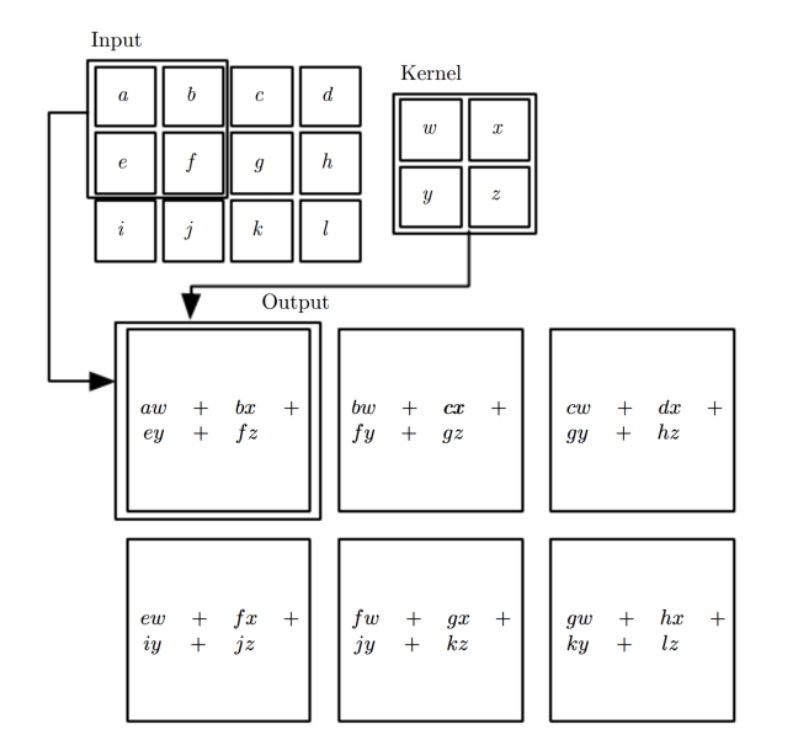
\includegraphics[scale=0.75]{sections/chapter-06/images/2-d-convolution-example.png}
%     \caption[Convolución 2D]{Convolución 2D. Imagen extraída de \href{https://www.deeplearningbook.org}{\textit{"Deep Learning Book"}}}
%     \label{fig:2d-convolution-example}
% \end{figure}

% \indent En el ejemplo de la Figura \ref{fig:2d-convolution-example} la imagen, $I \in \mathbb{R}^{3\times4}$ y el filtro, $K \in \mathbb{R}^{2 \times 2}$ con un $s = 1$ y $p = 0$, se obtiene una salida de $2 \times 3 \times 1$ ($C_0$ es 1). \\
% \indent Las operaciones de convolución son combinadas con una función de activación $\phi$ (generalmente la función \acrshort{relu}). Si se considera un filtro de $k \times k$, si $\mathbf{x}$ es una porción $k \times k $ de la imagen, la activación se obtiene tras deslizar una ventana de $k \times k$ y computando $z(\bm{x})=\phi(\bm{K} \cdot \bm{x}+\bm{b})$, donde $\bm{b}$ es el sesgo. 

% \subsection{Pooling layer}

% \indent Las \acrshort{cnn} tiene capas que permiten reducir las dimensiones, también referido como submuestreo, tomando la media o el máximo en porciones de la imagen (\textit{mean-pooling} o \textit{max-pooling}). A su vez, este tipo de capas tienen, al igual que las capas convolucionales, un paso o stride. Otra propiedad, es la de hacer la red menos sensible a pequeñas transiciones de la imagen de entrada. 

% \subsection{Fully-connected layers}

% \indent Luego de haber aplicado varias capas convolucionales, las \acrshort{cnn} terminan con una \textit{fully-connected layer}. El tensor a la salida de estas capas son transformadas en vectores como entradas a perceptrones.

\section{Redes neuronales recurrentes} \label{sec:rnn}

\indent A fin de inferir data secuencial, tal como texto o señales en el tiempo, aparecen las redes neuronales
recurrentes. La forma más simple de una red neuronal recurrente tiene múltiples copias de la misma red, cada una
pasando información a su sucesora. La primer red neuronal recurrente, era una \acrshort{mlp} con un bucle hacia si
misma. Definiendo $x(t)$, $\hat{y}(t)$, $\hat{z}(t)$ como la entrada, la salida y la capa intermedia en tiempo $t$
respectivamente.

\begin{align*}
  \hat{y}^{(k)}(t) &= \sum_{i=1}^{I} \bm{W}_i^{(k)} \hat{z}_i(t) + \bm{b}^{(k)} \\
  \hat{z}_i(t) &= \sigma\left(\sum_{j=1}^J w_{i,j}x_j(t) + \sum_{l=1}^I \Tilde{w}_{i,l} \hat{z}_l(t-1) + b_i \right)
\end{align*}

\indent Donde $\sigma$ es la función de activación. Las neuronas que son retroalimentadas asimismas, se denominan
\textit{context units} o unidades contextuales. Estos modelos y variaciones del mismo se han utilizado en el campo
del análisis lingüístico. Aunque, nuevas arquitecturas se han desarrollado para abordar estos problemas.

\subsection*{Long Short-Term Memory}

\indent Las RNN han sido exitosas en varias aplicaciones como han de ser reconocimiento del habla, traducción, entre
otros. Este éxito se debe a la eficiencia de las redes \acrshort{lstm}, que es una especie de red recurrente. Las
redes \acrshort{lstm} fueron introducidas por Hochreiter y Schmidhuber (1997) \cite{pp:hochreiter-schmidhuber} y
fueron creadas con el propósito de aprender dependencias a largo plazo. Una celda \acrshort{lstm} comprende, en un
instante $t$, un estado $C_t$ y una salida $h_t$. Como entrada, la celda requiere $x_t$, $C_{t-1}$, $h_{t-1}$.
Dentro de la celda, existen compuertas o \textit{gates} que permiten, o no, el paso de información. Este
comportamiento está dado por el siguiente conjunto de ecuaciones.

\begin{itemize}
  \item \textit{Update gate H}
  \begin{align}
    u_t = \sigma(\bm{W}^u h_{t-1} + \bm{I}^u x_t + b^u)
  \end{align}

  \item \textit{Forget gate H}
  \begin{align}
    f_t = \sigma(\bm{W}^f h_{t-1} + \bm{I}^f x_t + b^f)
  \end{align}

  \item \textit{Cell candidate H}
  \begin{align}
    \Tilde{C}_t = \mathrm{tanh}(\bm{W}^c h_{t-1} + \bm{I}^c x_t + b^c)
  \end{align}

  \item \textit{Cell output H}
  \begin{align}
    C_t = f_t \odot C_{t-1} + u_t \odot \Tilde{C}_t
  \end{align}

  \item \textit{Output gate H}
  \begin{align}
    o_t = \sigma(\bm{W}^o h_{t-1} + \bm{I}^o x_t + b^o)
  \end{align}

  \item \textit{Hidden output H}
  \begin{align}
    h_t = o_t \odot \mathrm{tanh}(C_t)
  \end{align}

  \item \textit{Output K}
  \begin{align}
    y_t = \mathrm{softmax}(\bm{W} \cdot h_t + b)
  \end{align}

  \item \textit{Recurrent weights H $\times$ H}
  \begin{align}
    \bm{W}^u, \bm{W}^f, \bm{W}^c, \bm{W}^o
  \end{align}

  \item \textit{Input weights N $\times$ H}
  \begin{align}
    \bm{I}^u, \bm{I}^f, \bm{I}^c, \bm{I}^o
  \end{align}

  \item \textit{Biases}
  \begin{align}
    b^u, b^f, b^c, b^o
  \end{align}
\end{itemize}

\indent La Figura \ref{fig:lstm-schematic} refleja la diferencia entre una celda RNN tradicional y una celda
\acrshort{lstm}. Una celda RNN contiene sólo una capa. En cambio, la celda \acrshort{lstm} contiene 4 capas dadas
por los bloques amarillos, interactuando entre ellas como se describen en las ecuaciones anteriores.

\begin{figure}[H]
  \centering
  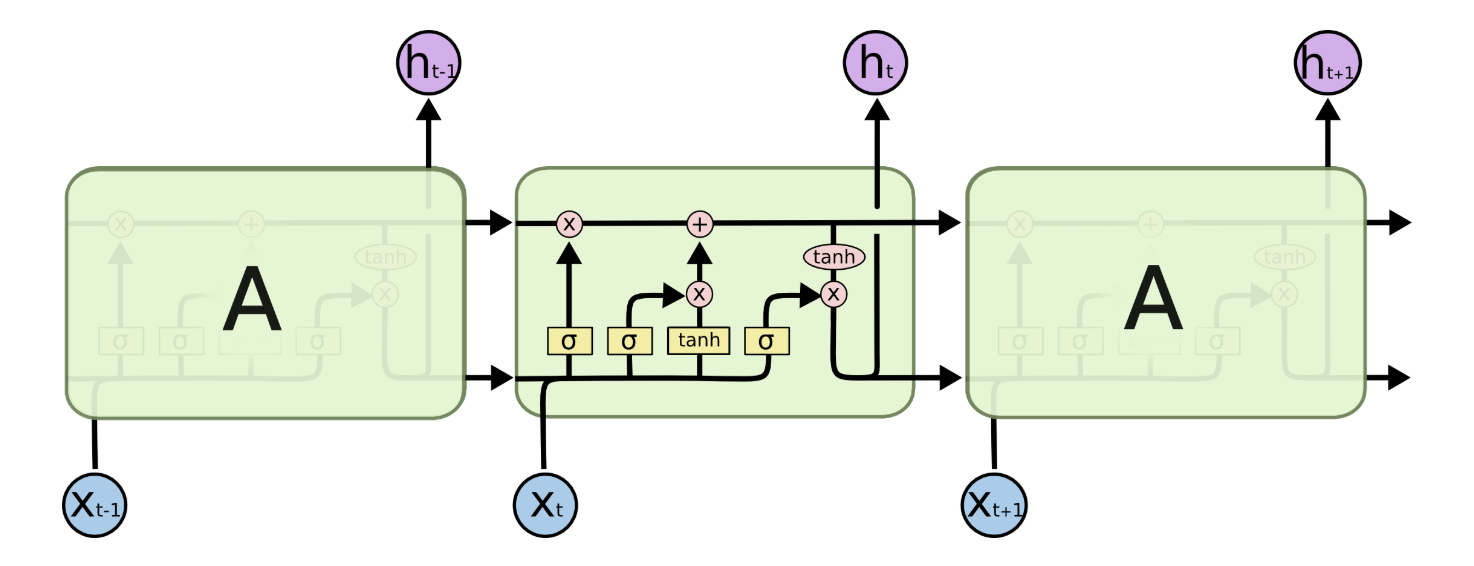
\includegraphics[scale=0.5]{sections/chapter-06/images/lstm-schematic.png}
  \caption[Diagrama de una red \acrshort{lstm}]{Diagrama de una red \acrshort{lstm}. Imagen extraída de
  \href{http://colah.github.io/posts/2015-08-Understanding-\acrshort{lstm}s/}{\textit{"Understanding \acrshort{lstm}
  Networks"}}}
  \label{fig:lstm-schematic}
\end{figure}

\indent Las redes \acrshort{lstm} son las elegidas en este trabajo. La particularidad de estas redes, como se ha
mencionado anteriormente, es la eficiencia para los problemas de señales en el tiempo.

\section{Sobre-entrenamiento}

\indent Estadísticamente hablando sobre-entrenamiento (\textit{overfitting}) se produce cuando un modelo corresponde
exactamente al conjunto de datos al que utiliza para estimar sus parámetros. Esto produce que predecir observaciones
futuras sea confiable. Un modelo sobre-entrenado generalmente tiene muchos más parámetros de los que se pueden
justificar con los datos de entrenamiento. Esencialmente, un modelo de estas características tiene por aprender
información descorrelacionada con los datos, por ejemplo ruido, como si fuese información representativa del modelo. \\
\indent Existe otro fenómeno de los modelos estadísticos, denominado sub-entrenamiento (\textit{underfitting}), que
contrario al sobre-entrenamiento ocurre cuando el modelo no es capaz de capturar la estructura de los datos, y sus
parámetros quedan en un estado indefinido.

\subsection*{Validación cruzada} \label{subsec:cross-validation}

\indent Antes de entrar en detalle en la extracción de los atributos tiempo-frecuencia, es necesario definir el
método de entrenamiento elegido en este trabajo. \\
\indent Validación cruzada (\textit{cross-validation}) es un método de validación de un modelo para analizar los
resultados estadísticos tal que éstos se encuentren los más generalizado a cualquier set de datos. Es comúnmente
usado donde el objetivo es la predicción, y se quiere saber cuán exacto y preciso el modelo predictivo es en la
práctica. En un problema de predicción, se define un set de datos de entrenamiento y otro conunto de datos de
evaluación. El primero, es un conjunto de datos en el cual el modelo predictivo estimará sus parámetros para luego
predecir datos que no hayan sido visto nunca. Aquí es cuando entra el conjunto de datos de evaluación, que va a ser
visto por primera vez por el modelo. Este método tiene como objetivo solucionar el problema de sobre-entrenamiento. \\
\indent Existen varias técnicas dentro de validación cruzada. En este trabajo se hará hincapié en el denominado
\textit{K-Folds}. Éste consiste en dividir el set completo de datos en $K$ grupos (generalmente es común utilizar $K
= 10$). El entrenamiento por ende se realizará $K$ veces, eligiendo en cada iteración un grupo de evaluación que no
haya sido elegido previamente. El resto de los grupos se utilizarán como entrenamiento. De esta manera se computarán
todas las métricas elegidas, $K$ veces y se computará la media, y el desvío de cada una de ellas.

\section{Métricas} \label{sec:metrics}

\indent Determinar métricas de error es fundamental a la hora de evaluar cuáles son los próximos pasos a seguir. \\
\indent Hay que tener en cuenta que en algunas aplicaciones es prácticamente imposible obtener un error nulo. El
error de Bayes define el mínimo error que se puede esperar alcanzar, aún obteniendo una cantidad infinita de datos y
recuperando la verdadera función de distribución. Este se debe a que los atributos pueden no contener toda la
información que se necesita para explicar la variable de salida o porque el sistema a analizar puede ser
intrínsecamente estocástico. En la práctica uno siempre va a estar limitad por una cantidad finita de datos. \\
\indent La cantidad de datos puede estar limitada por varios motivos. Por ejemplo, cuando el objetivo es construir
un producto o servicio comercializable, uno puede siempre conseguir más datos pero es necesario evaluar cuál es el
costo del mismo comparado a tratar de reducir el error. La recolección de datos implica tiempo, dinero y esfuerzo
humano. Un ejemplo típico del esfuerzo humano, cuando se necesita conseguir datos de un paciente clínico por medio
de técnicas invasivas. En el ámbito académico o de investigación, cuando el objetivo es responder una pregunta
científica sobre qué algoritmo tiene mejor rendimiento en base a un estándar (\textit{benchmark}), no es posible
agregar más datos. \\
\indent En muchas aplicaciones la exactitud (\textit{accuracy}) alcanza para definir el rendimiento de los
algoritmos. Sin embargo, en muchas ocasiones esto no es así. Es el ejemplo de la detección de una rara enfermedad,
en la que una persona en un millón padecen esta enfermedad. Por ende, una forma fácil de alcanzar $99.9999\%$ de
exactitud es simplemente diciéndole al equipo que reporte que en todos los casos la enfermedad se encuentra ausente.
Claramente, esta métrica no es útil y una forma de resolver esto es utilizando otras métricas como son la precisión
y sensibilidad (\textit{recall}). La precisión se define como la cantidad de detecciones que el algoritmo definió
como correctas y sensibilidad es la cantidad de eventos verdaderos que fueron detectados. Un detector que dice que
nadie tiene esta enfermedad, tiene $100\%$ de precisión pero 0 sensibilidad. Un detector que dice que todos tienen
la enfermedad, tiene $100\%$ de sensibilidad pero precisión igual a la cantidad de las personas que sí la tienen, $0
.0001\%$ en este ejemplo. En muchas aplicaciones, es bueno resumir esta información en una sola métrica. Esta
métrica se conoce como métrica F$_1$.

\begin{align}
  F_1 = 2\frac{PR}{P+R}
\end{align}

\indent Otra opción es reportar el área bajo la curva P-R, donde en el eje de abscisas se encuentra R y en el eje de
ordenadas, P. \\
\indent Muchas otras métricas son posibles. En distintas aplicaciones especializadas, existen métricas
característica de ese campo. \\
\indent Una manera de mostrar rendimiento de un algoritmo de estimación, es por medio de la matriz de confusión.
Esta matriz representa en sus columnas las clases verdaderas y las filas contienen a las clases estimadas. Esta
matriz resume distintas métricas, de las cuales es posible obtener resultados. Estas métricas se especifican a
continuación.

\begin{itemize}
  \item Sensibilidad
  \begin{align}
    \acrshort{tpv} = \frac{\acrshort{tp}}{\acrshort{tp}+\acrshort{fn}}
  \end{align}

  \item Especificidad
  \begin{align}
    \acrshort{tnr} = \frac{\acrshort{tn}}{\acrshort{tn}+\acrshort{fp}}
  \end{align}

  \item Precisión
  \begin{align}
    \acrshort{ppv} = \frac{\acrshort{tp}}{\acrshort{tp}+\acrshort{fp}}
  \end{align}

  \item Valor Predictivo Negativo
  \begin{align}
    \acrshort{npv} = \frac{\acrshort{tn}}{\acrshort{tn}+\acrshort{fn}}
  \end{align}

  \item Tasa de error
  \begin{align}
    \acrshort{fnr} = \frac{\acrshort{fn}}{\acrshort{fn}+\acrshort{tp}}
  \end{align}

  \item Tasa de falsos positivos
  \begin{align}
    \acrshort{fpr} = \frac{\acrshort{fp}}{\acrshort{fp}+\acrshort{tn}}
  \end{align}

  \item Tasa de descubrimiento
  \begin{align}
    \acrshort{fdr} = \frac{\acrshort{fp}}{\acrshort{fp}+\acrshort{tp}}
  \end{align}

  \item Tasa de omisión
  \begin{align}
    \acrshort{for} = \frac{\acrshort{fn}}{\acrshort{fn}+\acrshort{tn}}
  \end{align}

  \item Exctitud
  \begin{align}
    \acrshort{acc} = \frac{\acrshort{tp}+\acrshort{tn}}{\acrshort{tp}+\acrshort{tn}+\acrshort{fn}+\acrshort{fp}}
  \end{align}

  \item Puntaje F$_1$
  \begin{align}
    F_1 = \frac{2\acrshort{tp}}{2\acrshort{tp}+\acrshort{fp}+\acrshort{fn}}
  \end{align}
\end{itemize}

\indent Las métricas que aquí se trabajarán son exactitud ($ACC$), precisión ($P_+$), sensibilidad ($Se$) y $F_1$.
Los motivos de esta decisión es la naturaleza de la aplicación y por comparación de desempeño con otros trabajos
publicados. \\
\indent \acrshort{tp} define a los verdaderos positivos y \acrshort{tn} a los verdaderos negativos. En base a estos
dos parámetros se pueden calcular todas las métricas mencionadas. Por otro lado, cabe destacar que dependiendo de la
cantidad de clases que el problema posea, es necesario computar \acrshort{tp} y \acrshort{tn} para cada una de ellas
. Más adelante, se dará un ejemplo en el caso de 4 clases.

  \chapter{Implementación} \label{ch:results}

\indent Este capítulo tiene como objetivo mostrar y reflejar el trabajo hecho. El preprocesamiento y el
procesamiento se ha explicado en capítulos anteriores. Aquí se mencionarán los elementos necesarios para la ejecutar
la clasificación, como por ejemplo el \textit{framing}. Se describirá la arquitectura de la red \gls{lstm}
utilizada, junto a la descripción de sus capas intermedias y los hiperparámetros seleccionados. \bigskip

\subsection*{Diagrama de flujo del sistema} \label{subsec:flow-diagram}

\indent Antes de abordar cada uno de los distintos pasos, se ilustra una diagrama de flujo de todo el sistema.
Empezando desde el filtrado lineal para eliminar ruido que corrompa la señal, pasando por la extra cción de marcas y
la extracción de atributos para dar finalmente con la clasificación de los estados de la señal (diagrama que
contempla tanto la etapa de entrenamiento como la de evaluación).


\begin{figure}[H]
  \centering
  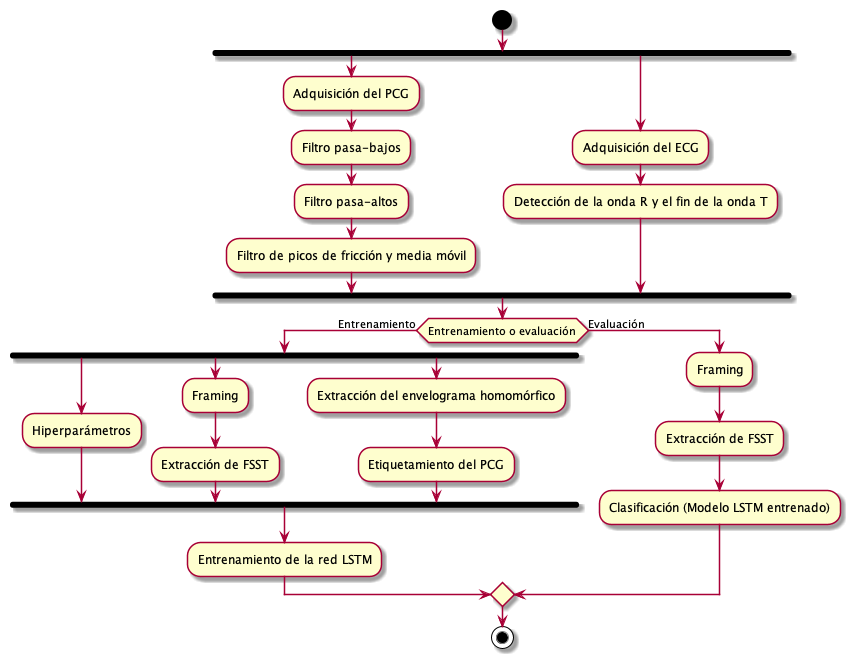
\includegraphics[scale=0.7]{sections/chapter-07/images/flow-diagram.png}
  \caption[Diagrama de flujo del sistema]{Diagrama de flujo del sistema.}
  \label{fig:flow-diagram}
\end{figure}

\newpage

\section{Encuadrado} \label{sec:framing}

\indent El proceso de dividir una señal de una dada longitud $L$ en señales de igual longitud se denomina encuadrado
(\textit{framing}). Ésto es necesario debido a que las señales de fonocardiograma poseen longitudes diferentes. La
base de datos, ya se ha mencionado, tienen adquisiciones de distintas duraciones, y la arquitectura propuesta más
adelante, necesita como entrada $M$ señales con una longitud $N$ fija. \\
\indent El encuadrado es posible realizarlo con una ventana cuadrada, o cualquier otro tipo de ventana. La elección
de la ventana esta dada por el problema a resolver. En este caso, se utilizó una ventana cuadrada. \bigskip

\indent Dada una señal $\mathbf{x} \in \mathbb{R}^T$, se desea obtener una cantidad $Q$ de señales. Este valor está
dada por la ecuación \ref{eq:q}

\begin{align}
  \label{eq:q}
  Q := \left[\frac{T-1-N}{\tau}\right]
\end{align}

\indent La notación $[...]$ implicá el entero más cercano. El deslizamiento de la ventana está dado por $\tau$,
dependiendo de $N$ y de $\tau$, se define si existe solapamiento u \textit{overlapping}.

\begin{align}
  O =
  \begin{cases}
    1, \; 0 \leq \tau \leq N \\
    0, \; \tau \geq N
  \end{cases}
\end{align}

\indent De esta manera, queda definido el vector, $\bm{\Tilde{x}}_k \in \mathbb{R}^{N}$ según la siguiente ecuación.

\begin{align}
  \bm{\Tilde{x}}_k = \left[\begin{array}{cccc}
    \bm{x}_{\tau \cdot k} &
    \bm{x}_{\tau \cdot k+1} &
    \dots & \bm{x}_{\tau \cdot k + N - 1}
  \end{array}\right]^\top
\end{align}

\begin{align}
  \bm{X}_j = \left[\begin{array}{cccc}
    \bm{\Tilde{x}}_1 &
    \bm{\Tilde{x}}_2 &
    \dots &
    \bm{\Tilde{x}}_Q
  \end{array}\right]^\top
\end{align}

\indent Donde $k = 1,2,...,Q$. Por último, una vez obtenidos los $Q$ cuadros para una señal $j$, donde $j = 1,2,...,
D$ y $D$ la cantidad total de señales, se itera sobre todo el set de datos y se genera la matriz $\bm{H} \in
\mathbb{R}^{M \times N}$.

\begin{align}
  \bm{H} = \left[\begin{array}{cccc}
    \bm{X}_1 &
    \bm{X}_2 &
    \dots &
    \bm{X}_D
  \end{array}\right]^\top
\end{align}

\indent Es importante tener en cuenta que en los casos que $\frac{T-1-N}{\tau}$ no sea entero, quedarán muestras
(generalmente del final) sin incluir en los datos, las cuales serán descartadas.

\section{Extracción de atributos}

\indent Una vez hecho el acondicionamiento de la señal (filtrado, normalización en términos de energía) y los
cuadros listos, se procede a extraer los features necesarios a introducir al clasificador. Los features extraídos
son obtenidos por medio de la \gls{fsst}, el clasificador es una red diseñada con celdas \gls{lstm}. \bigskip

\indent Para la extracción de features en tiempo-frecuencia se utilizó la \gls{fsst}. Esta se aplica sobre
segmentos de señal extraídos del proceso de encuadrado. \\
\indent En esta ocasión, no se utiliza solapamiento de cuadros (\textit{frames}), con lo cual cada segmento de señal
posee información única a excepción de una muestra. Previamente, se eligen las señales mayores o iguales a una
longitud $N$, cuyo valor va a ser el largo de cada segmento. \\
\indent A cada segmento se le aplica la transformada con una ventana definida. La ventana elegida es la ventana de
Kaiser con una longitud $L = 128$ y un $\beta = 0.5$. Esta ventana fue seleccionada dado a que su objetivo es
maximizar la relación de energía entre lóbulo principal y sus lóbulos secundarios, reduciendo los efectos del ruido
en esas bandas de frecuencia y mejorando la calidad de la transformada.

\begin{figure}[H]
  \centering
  \begin{subfigure}{\textwidth}
    \centering
    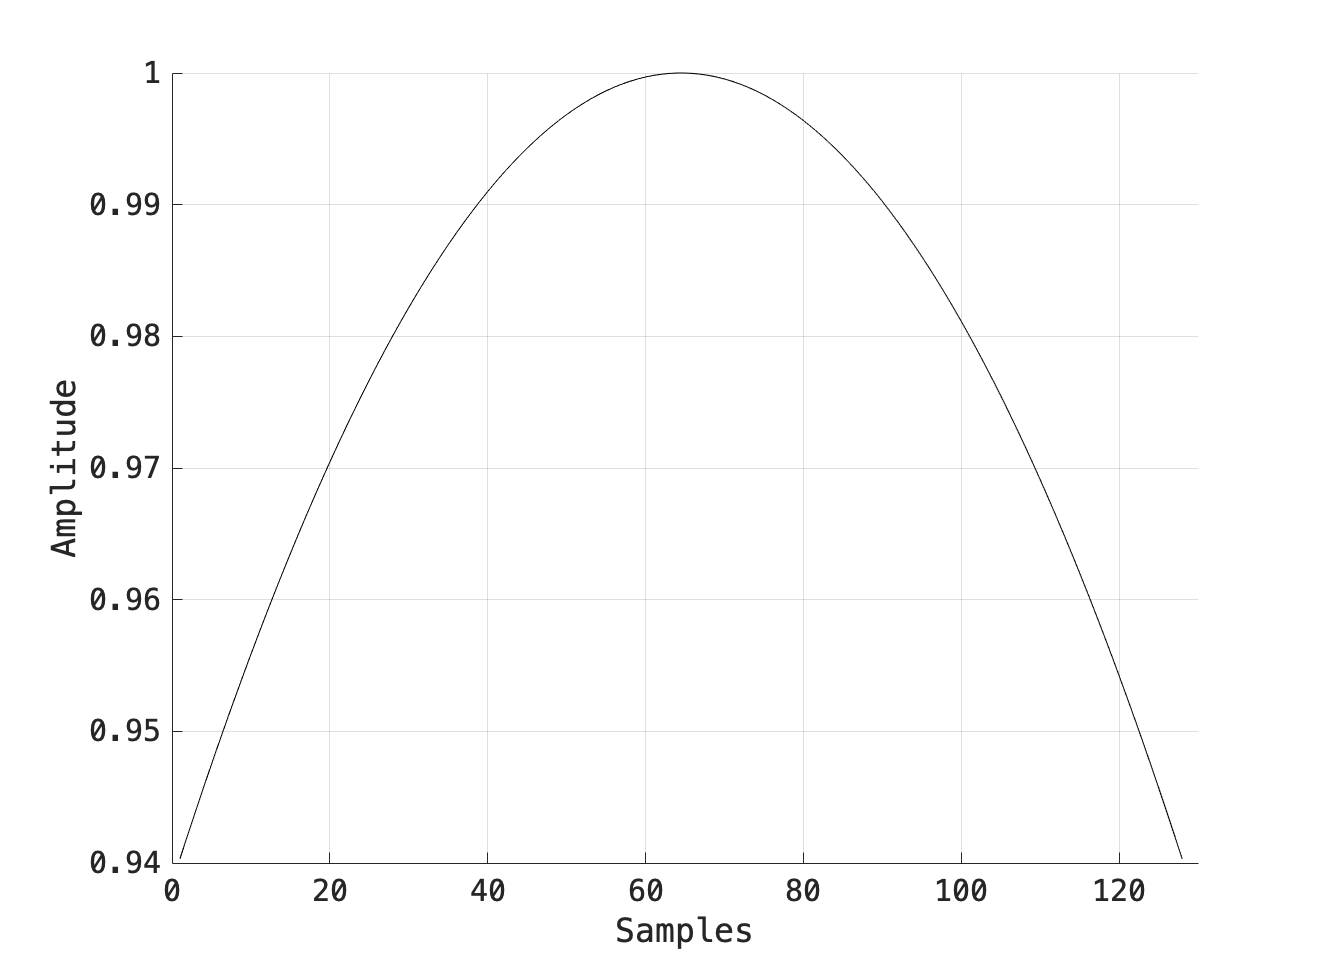
\includegraphics[scale=0.23]{sections/chapter-07/images/kaiser-window.png}
    \caption[Ventana de Kaiser]{Ventana de Kaiser. La ventana diseñada con un largo $L = 128$ y un $\beta = 0.5$.}
  \end{subfigure} \\
  \begin{subfigure}{\textwidth}
    \centering
    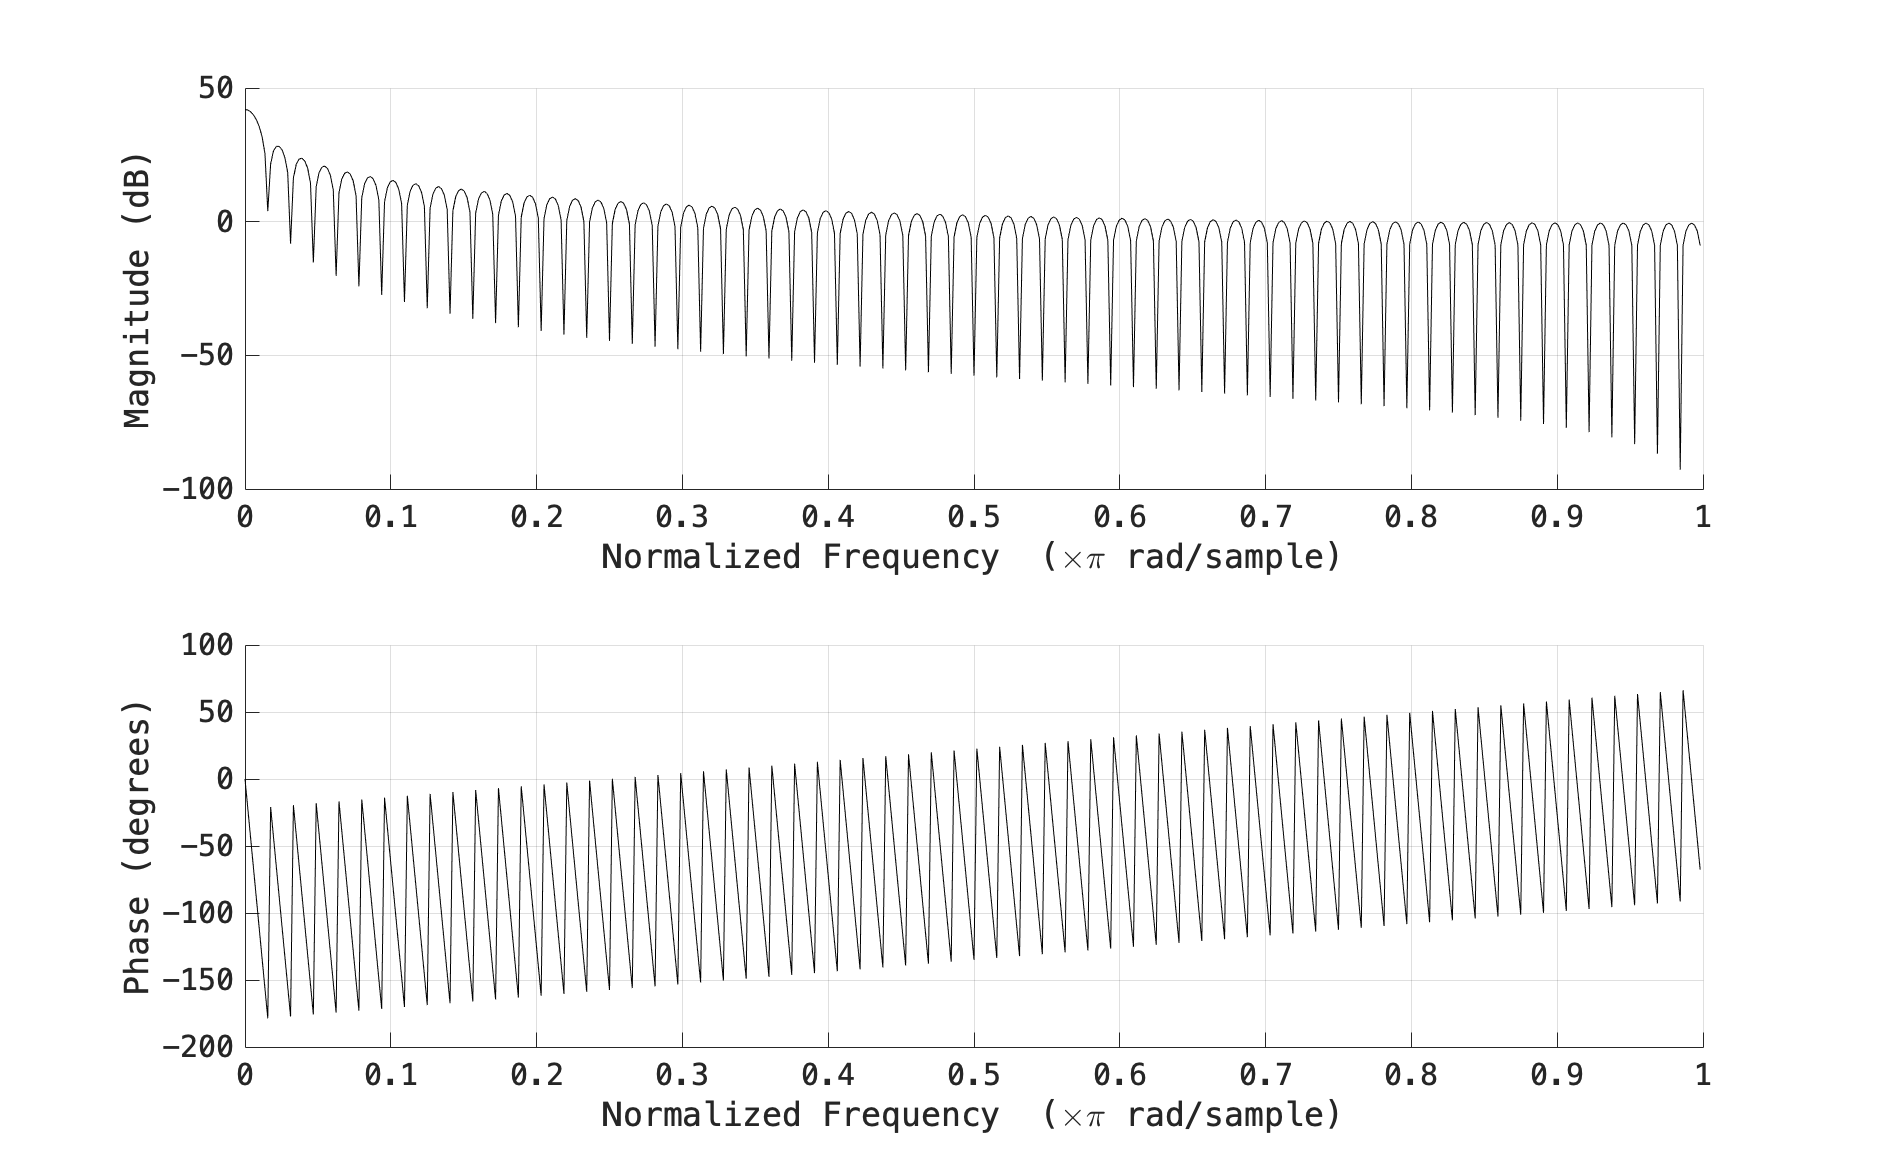
\includegraphics[scale=0.21]{sections/chapter-07/images/kaiser-window-freqz.png}
    \caption[Respuesta en frecuencia de la ventana de Kaiser]{Respuesta en frecuencia de la ventana de Kaiser. La
    respuesta se encuentra en decibeles y se ilustra tanto la magnitud como la fase.}
  \end{subfigure}
  \label{fig:kaiser-window-plot}
\end{figure}

\indent El parámetro $\beta$ se calcula en base a la ecuación \ref{eq:kaiser-beta}.

\begin{align} \label{eq:kaiser-beta}
  \beta = \begin{cases}
    0.1102(\alpha-8.7), \; \alpha > 50 \\
    0.5842(\alpha-21)^{0.4}+0.7886(\alpha-21), \; 50 \geq \alpha \geq 21, \\
    0, \; \alpha \geq < 21
  \end{cases}
\end{align}

Y la banda de transición, según el largo de la ventana, se calcula despejando $\Delta\omega$ de la ecuación
\ref{eq:kaiser-transition-band}.

\begin{align} \label{eq:kaiser-transition-band}
  L = \frac{\alpha-8}{2.285\Delta\omega} + 1
\end{align}

\indent En la Figura \ref{fig:pcg-fsst} se ilustra la transformada extraída de una señal de fonocardiograma. Se
visualiza claramente el contenido frecuencia en los distintos sonidos del fonocardiograma y la periodicidad de los
mismos. Por otro lado, se muestra que por debajo de frecuencias de los 20 Hz y por encima de los 200 Hz no hay
contenido espectral relevante en cuanto a energía. La mayor cantidad de contenido frecuencia se encuentra entre
dicho rango. Por ende, se extraen los features entre 20-200 Hz como entrada al clasificador.

\begin{figure}[H]
  \centering
  \begin{subfigure}{\textwidth}
    \centering
    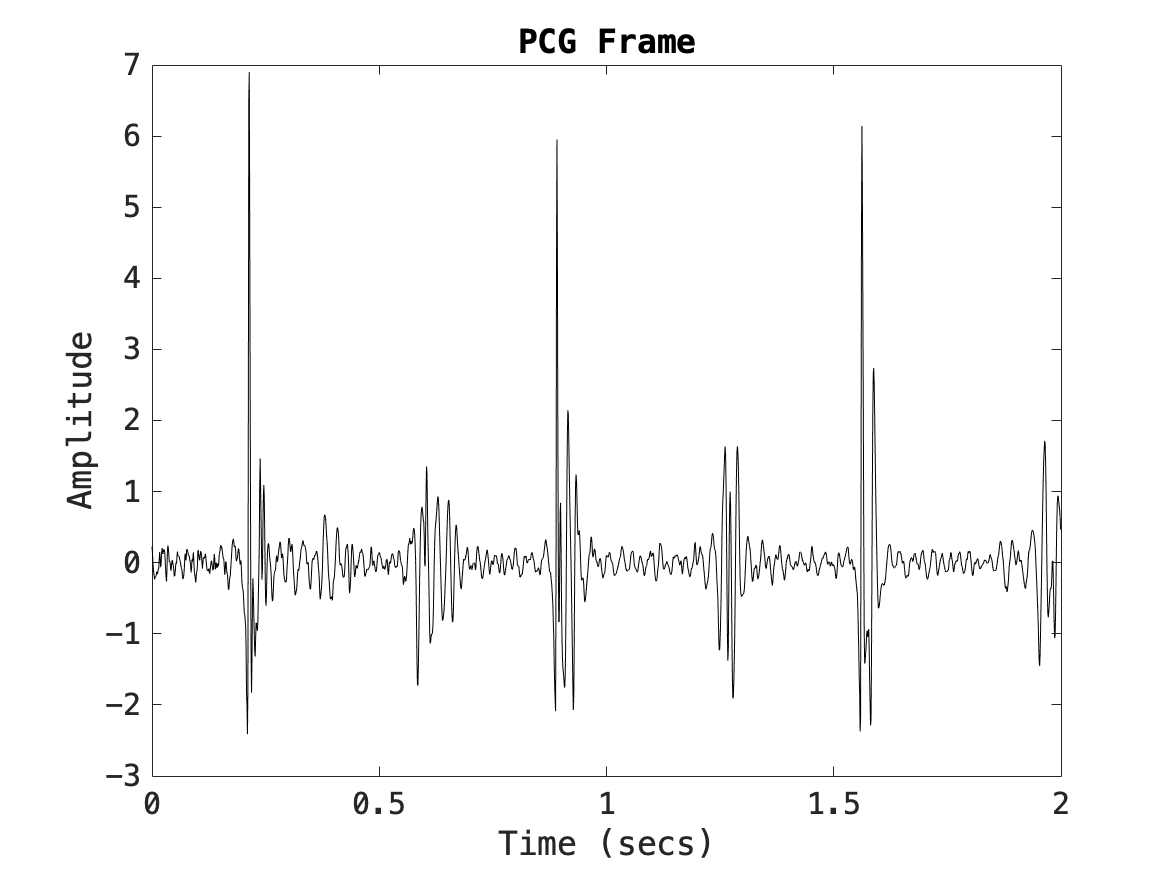
\includegraphics[scale=0.27]{sections/chapter-07/images/pcg-frame.png}
    \caption[Segmento de una señal de fonocardiograma]{Segmento de una señal de fonocardiograma.}
    \label{fig:pcg-frame}
  \end{subfigure} \\
  \begin{subfigure}{\textwidth}
    \centering
    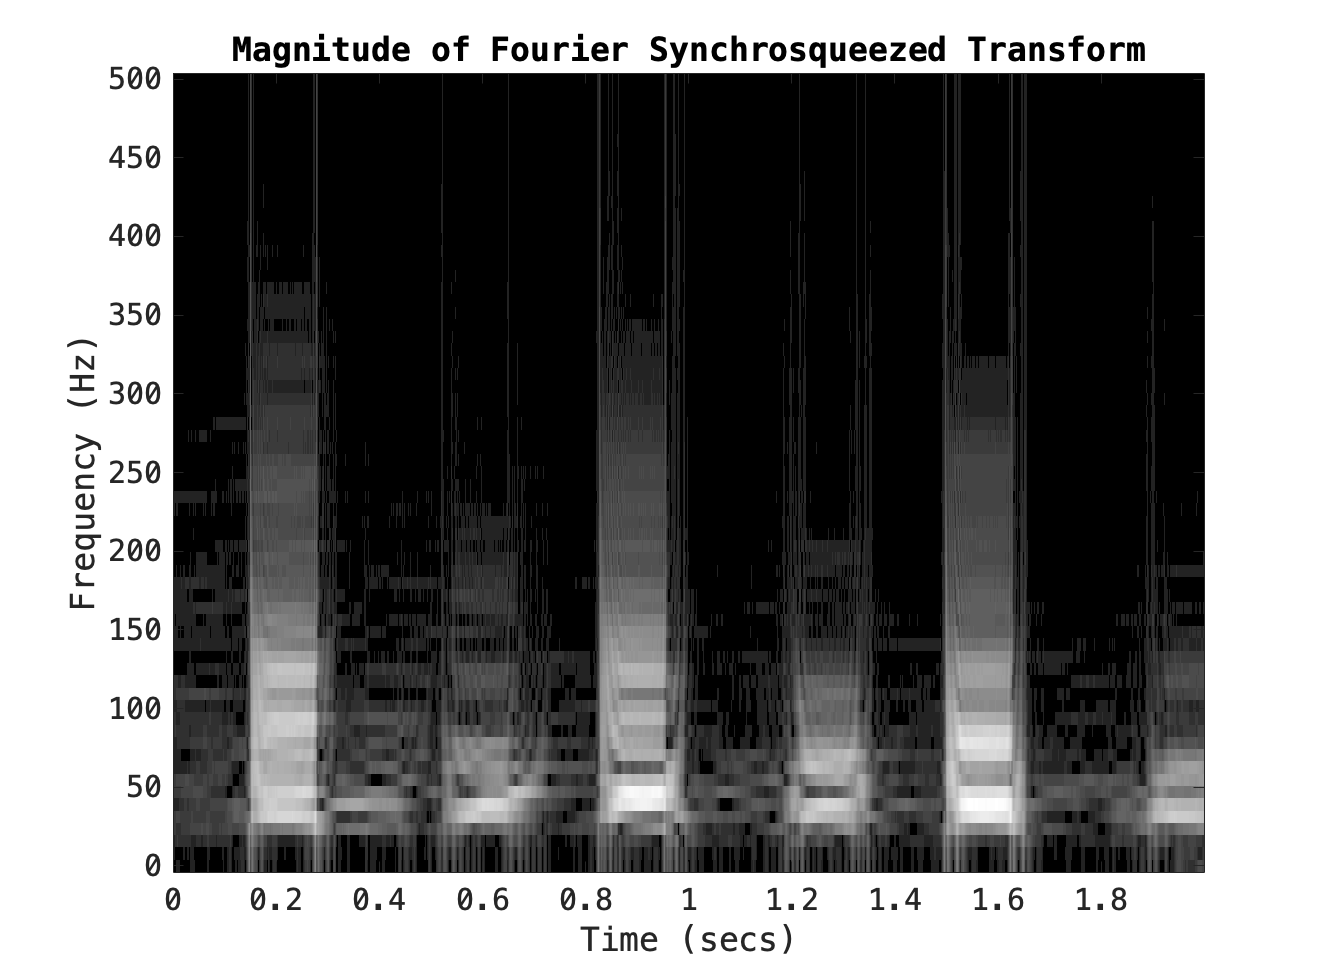
\includegraphics[scale=0.25]{sections/chapter-07/images/fsst-plot.png}
    \caption[Magnitud de la \gls{fsst} aplicada a un segmento de señal de fonocardiograma]{Magnitud de la
    \gls{fsst} aplicada a un segmento de señal de fonocardiograma.}
    \label{fig:fsst-diagram}
  \end{subfigure}
  \caption[Ejemplo de la transformada \gls{fsst} a un segmento de señal de \gls{pcg}]{Ejemplo de la
  transformada \gls{fsst} a un segmento de señal de \gls{pcg}.}
  \label{fig:pcg-fsst}
\end{figure}

\indent Se ve claramente como la mayor energía frecuencial corresponde a los instantes donde se producen los sonidos
fundamentales. También, en este ejemplo, hay energía proveniente de otras fuentes de ruido, entre los instantes 1-1
.2 segundos.

\subsection{Modelo} \label{subsec:model}

\indent El clasificador es una red neuronal \gls{lstm} como se ha mencionado anteriormente. Los parámetros a
estimar del modelo pertenecen a la capa \gls{lstm}. Por otro lado, es predefinir los hiperparámetros de la red
neuronal. Además de la capa recurrente, a una red neuronal la componen otras capas intermedias y una capa de entrada
y salida.

\subsubsection{Arquitectura}

\indent La arquitectura de la red neuronal consiste en de 5 capas. Una de entrada, una recurrente, una
\textit{fully-connected} con otra de softmax y una de salida. La arquitectura se ilustra en la Figura
\ref{fig:nn-architecture}.

\begin{figure}[H]
  \centering
  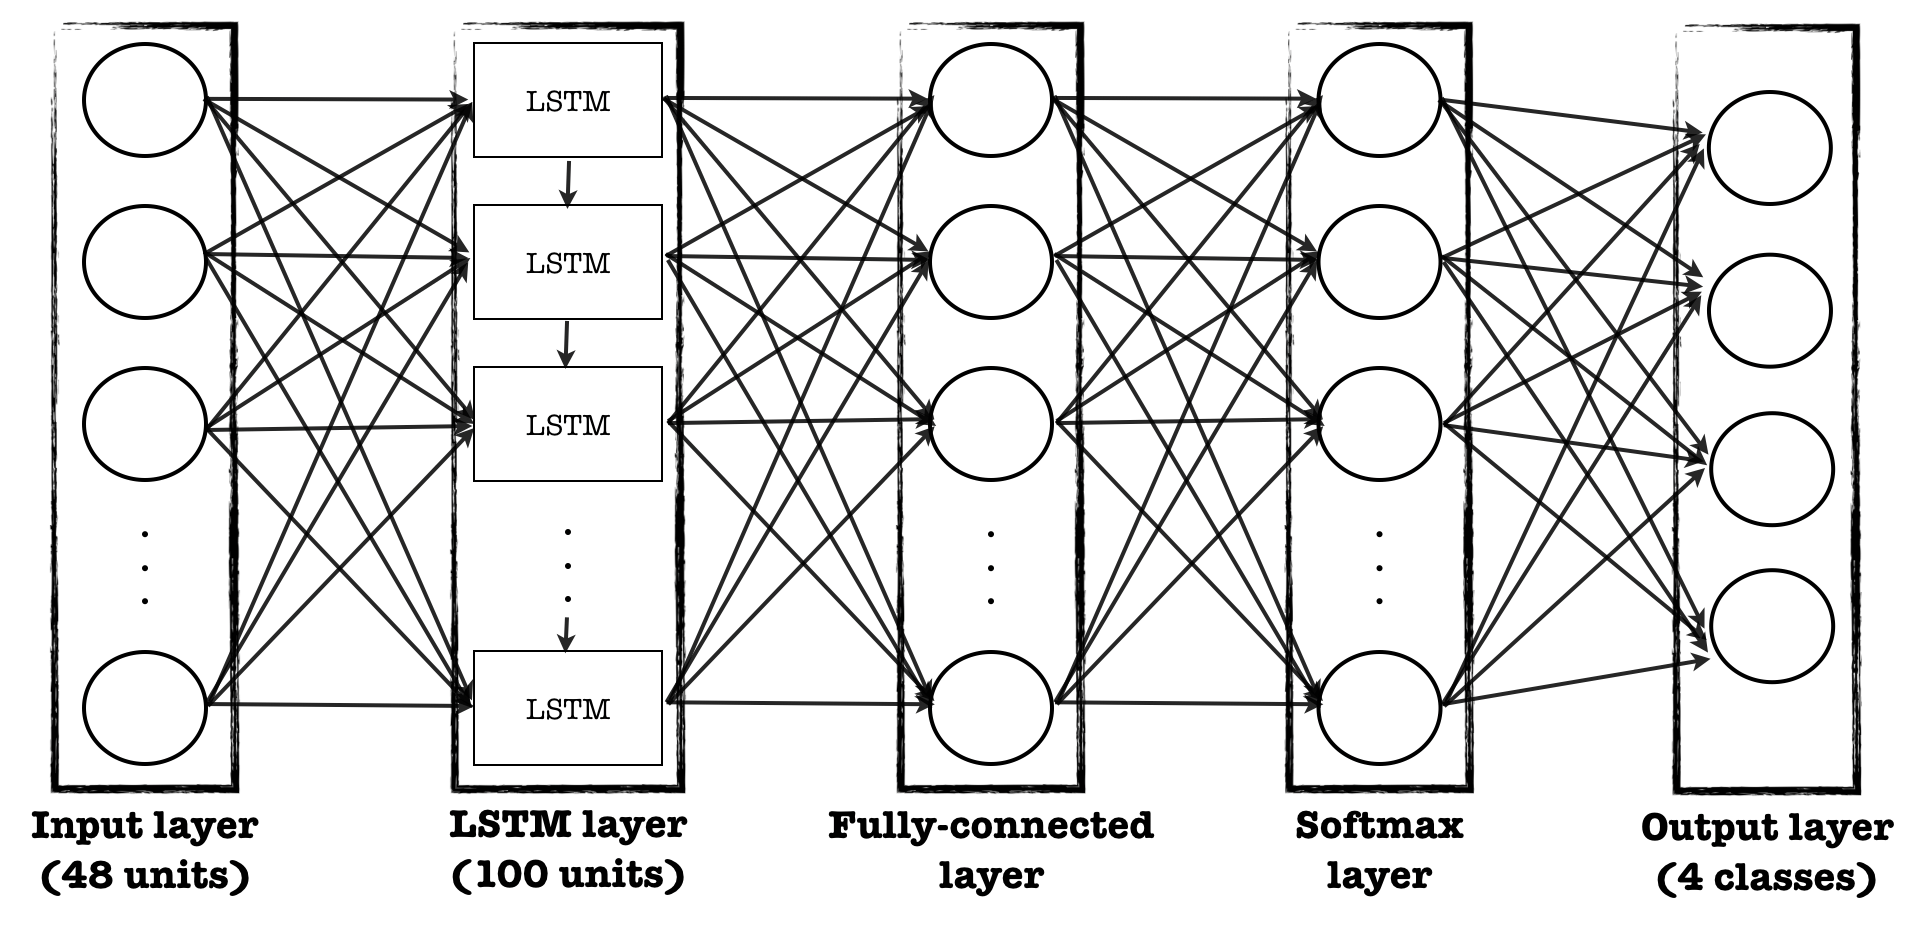
\includegraphics[scale=0.35]{sections/chapter-07/images/lstm-architecture.png}
  \caption[Arquitectura de la red neuronal]{Arquitectura de la red neuronal.}
  \label{fig:nn-architecture}
\end{figure}

\subsubsection{Hiperparámetros}

\indent Ya se ha visto que es necesario establecer hiperparámetros de la red. Para el entrenamiento se utiliza el
algortimo publicado en 2014 en la \gls{iclr} 2015, denominado \textit{Adam} \cite{pp:adam}. El algoritmo
introduce ciertos hiperparámetros además de los convencionales que es necesario definir a priori. \\*
\indent Los hiperparámetros utilizados en la implementación se listan a continuación \footnote{Los nombres de los
hiperparámetros se encuentran en inglés, dado a que no hay literatura en español y muchos de ellos no tienen
traducción}.

\begin{itemize}
  \item \texttt{MaxEpochs: 10}
  \item \texttt{MiniBatchSize: 50}
  \item \texttt{InitialLearngRate: 0.01}
  \item \texttt{LearnRateDropPeriod: 3}
  \item \texttt{LearnRateDropFactor: 0.1}
  \item \texttt{L2Regularization: 1e-04}
  \item \texttt{GradientDecayFactor: 0.9}
  \item \texttt{SquaredGradientDecayFactor: 0.99}
  \item \texttt{Epsilon: 1e-08}
  \item \texttt{GradientThreshold: 1}
\end{itemize}

\indent Generalmente, lo normal es elegir la cantidad de \textit{epochs} alrededor de 10. En disintas aplicaciones
se han utilizado un número entre $15-30$. Esto hace que el tiempo de entrenamiento sea aún mayor. Recordar que por
cada una de ellas todo el set de datos ha pasado por la red. Por temas de cómputo y tiempos, se decidió fijar la
cantidad de \textit{epochs} en el valor estándar. Por otro lado, bastante ligado a la cantidad de \textit{epochs} y
el tamaño del lote se definió por motivos computacionales, tiempo y desempeño de la red por medio de distintas
iteraciones. \\
\indent Otros parámetros de interés, son \textit{InitialLearnRate}, \textit{LearnRateDropPeriod} y
\textit{LearnRateDropFactor}. Éstos son necesarios dado a que el \textit{LearnRate} se modifica a lo largo de las
iteraciones, y con estos parámetros se define cada cuánto y por cuánto se reduce el mismo. En esta implementación se
definió que cada 3 \textit{epochs} se reduce un 1\%. \\
\indent Lo que se conoce como \textit{Regularization} intenta resolver el problema de generalización o
sobreentrenamiento en lo que respecta a los pesos de la red. También se lo denomina, en inglés, \textit{weight
decay}. Estos pesos se encuentran asociados a la función de costo y \textit{L2Regularization} se encuentra
representado como un factor. En esta implementación toma el valor de 1e-04. La función de costo, $E_R(\theta)$, con
el factor de regularización tiene la forma de la ecuación \ref{eq:l2-regularization}.

\begin{align} \label{eq:l2-regularization}
E_R(\theta) = E(\theta) + \lambda \Omega(w)
\end{align}

Donde,

\begin{align}
  \Omega(w) = \frac{1}{2} w^\top w
\end{align}

\indent $\Omega(w)$ es la función de regularización y $w$ son los pesos, la cual se encuentra multiplicada por el
factor $\lambda$ correspondiente a \textit{L2Regularization}. \bigskip

\indent Luego, los factores inherentes al algoritmo Adam, son \textit{GradientDecayFactor} y
\textit{SquaredGradientDecayFactor}. Normalmente en la mayoría de los casos toman el valor de $0.9$ y $0.99$
respectivamente. \\
\indent Adam utiliza medias móviles para actualizar los parámetros de la red. Estas medias se utilizan para el
gradiente y el gradiente al cuadrado, según las ecuaciones \ref{eq:gradient}, \ref{eq:squared-gradient}.

\begin{align} \label{eq:gradient}
  m_l = \beta_1 m_{l-1} + (1-\beta_1) \nabla E(\theta_l)
\end{align}

\begin{align} \label{eq:squared-gradient}
  v_l = \beta_2 v_{l-1} + (1-\beta_2) [\nabla E(\theta_l)]^2
\end{align}

Donde, $\beta_1$ y $\beta_2$ son los hiperparámetros \textit{GradientDecayFactor} y \textit{SquaredGradientDecayFactor}.

\begin{align} \label{eq:adam-update}
  \theta_{l+1} = \theta_l + \frac{\alpha m_l}{\sqrt{v_l}+\epsilon}
\end{align}

\indent La ecuación \ref{eq:adam-update} define cómo se actualizan los parámetros de la red con las medias móviles.
Por otro lado, si los gradientes durante varias iteraciones son similares, el uso de las medias móviles de los
gradientes permiten a la actualización de los parámetros tomar momento hacia una dirección. Existe la posibilidad de
que los gradientes sólo contengan ruido con lo cual, las medias móviles de los gradientes serán pequeñas y así
también actualización. Para ellos se elige un valor $\epsilon$ tal que la actualización esa no diverja, ya que
$\sqrt{v_l}$ puede ser muy pequeño. En muchas ocasiones se utiliza $\epsilon = 0.01$ pero en aplicaciones un valor
cercano a 1 funciona mejor. Queda definir el parámetro $\alpha$ como el \textit{LearnRate} mencionado. Es posible
que este parámetro tome diferentes valores para distintas capas intermedias y depende del algoritmo en cuestión. Es
por eso que no se puede definir un valor estándar de este hiperparámetro. \bigskip

\indent Por último, queda definir el hiperparámetro \textit{GradientThreshold}. Este umbral intenta acortar el
gradiente si los valores lo exceden. El método se basa en utilizar la norma L2 tal que si la norma del gradiente
excede el umbral, se escala el gradiente tal que su norma lo igual. En este caso el umbral toma el valor de 1.

\subsection{K-Folds} \label{subsec:k-folds}

\indent Recoradar que la técnica utilizada para resolver el problema de generalidad en el momento del entrenamiento
es la ya mencionada en el Capítulo \ref{ch:deep-learning}, validación cruzada (particularmente
\textit{10-Folds}). Para separar los fonocardiogramas en distintos grupos, se define el siguiente algoritmo. \bigskip

\indent Sea la señal de fonocardiograma $\mathbf{s}_i \in \mathbb{R}^N$, sus etiquetas (previamente calculadas)
$\mathbf{l}_i \in \mathbb{R}^N$ y la cantidad de \textit{folds} $K$. La cantidad de fonocardiogramas está dada por
el valor $L$, por lo tanto $i = 0,1,2,\dots,L-1$. \bigskip

\indent De esta manera se define $M$ como la cantidad de \gls{pcg} por \textit{fold}.

\begin{align}
  M = \left\lfloor \frac{L}{K} \right\rfloor
\end{align}

\indent Por lo tanto la ecuación \ref{eq:fold-selection} define cómo asignar cada \gls{pcg} a un \textit{fold}.

\begin{align} \label{eq:fold-selection}
 F_{n,j} = i, \quad (n \cdot M) < i < (n+1) \cdot (M-1)
\end{align}

\indent Con $i=0,1,2,\dots,M-1$ y $n = 0,1,2,\dots,K-1$. De esta manera se define la matriz $\bm{F} \in
\mathbb{R}^{K \times M}$, que contiene los indices correspondientes a cada \textit{fold}.

\begin{align}
  \bm{F} = \left[\begin{array}{ccccc}
    F_{0,0} & F_{0,1} & \dots & F_{0,M} \\
    F_{1,0} & F_{1,1} & \dots & F_{1,M} \\
    \vdots  & \vdots  & \ddots & \vdots \\
    F_{K,0} & F_{K,1} & \dots & F_{K,M}
  \end{array}\right]
\end{align}

\indent Si $\frac{L}{K}$ no fuese un número entero, significaría que no todos los \textit{folds} contendrán la misma
cantidad. La cantidad de señales huérfanas se calcula en la ecuación \ref{eq:pcg-lefts}.

\begin{align} \label{eq:pcg-lefts}
  L_{s} = \mathrm{mod}(L,K)
\end{align}

\indent En este momento es cuando se decide eliminar esas señales, agregar más para que la matriz $\mathbf{F}$ sea
consistente o se agregan de manera aleatoria a cualquier \textit{fold}.

Para definir los distintos grupos, los cuales serán $K$, cada grupo contenerá $K-1$ folds de entrenamiento y 1
\textit{fold} de evaluación. \\
\indent Se definen la matriz de entrenamiento, $\bm{T}_p \in \mathbb{R}^{K-1 \times M}$ y la matriz de evaluación
$\mathbf{E}_p \in \mathbb{R}^M$. Ambos asociados a un grupo $P \in \{0,1,2,\dots,K-1\}$

\begin{align}
  \mathrm{fil}_i(\bm{T}_p) = \mathrm{fil_j(\bm{F})}, \quad j \in \{0,1,2,\dots,K-1\}-\{p\}
\end{align}

\begin{align}
  \bm{E}_{p} = \mathrm{fil_p}(\bm{F})
\end{align}

\indent De esta manera, quedan definidos los grupos para realizar los K entrenamientos y ponderar métricas de
performance.

\section{Clasificación}

\indent La clasificación se realiza a partir de las probabilidades de la matriz $\bm{B} \in \mathbb{R}^{n \times 4}$.
Esta matriz es la que la capa de salida genera. En ella la se encuentra la probabilidad de que cada muestra de la
señal pertenezca a alguna clase. La forma de elegir la clase se muestra en la ecuación \ref{eq:class-definition}.
Esto es lo que generalmente la mayoría de las redes neuronales a su salida realizan como forma de clasificación, es
el caso de la segmentación mediante la una adaptación de la red neuronal \textit{U-Net} de Renna \textit{et al.}
\cite{pp:renna2018}.

\begin{align} \label{eq:class-definition}
C_i = \arg \underset{j}{\mathrm{max}} \; B_{i,j}
\end{align}


\indent Es necesario mencionar que en el entrenamiento de la red neuronal no se ha impuesto ninguna restricción de
transición de estados, a diferencia de lo que realmente sucede en el fonocardiograma. De esta manera, existen en la
predicción y por ende en la clasificación transiciones espurias que no corresponden. En la Figura
\ref{fig:spurious-transitions} se ilustra este fenómeno.

\begin{figure}[H]
  \centering
  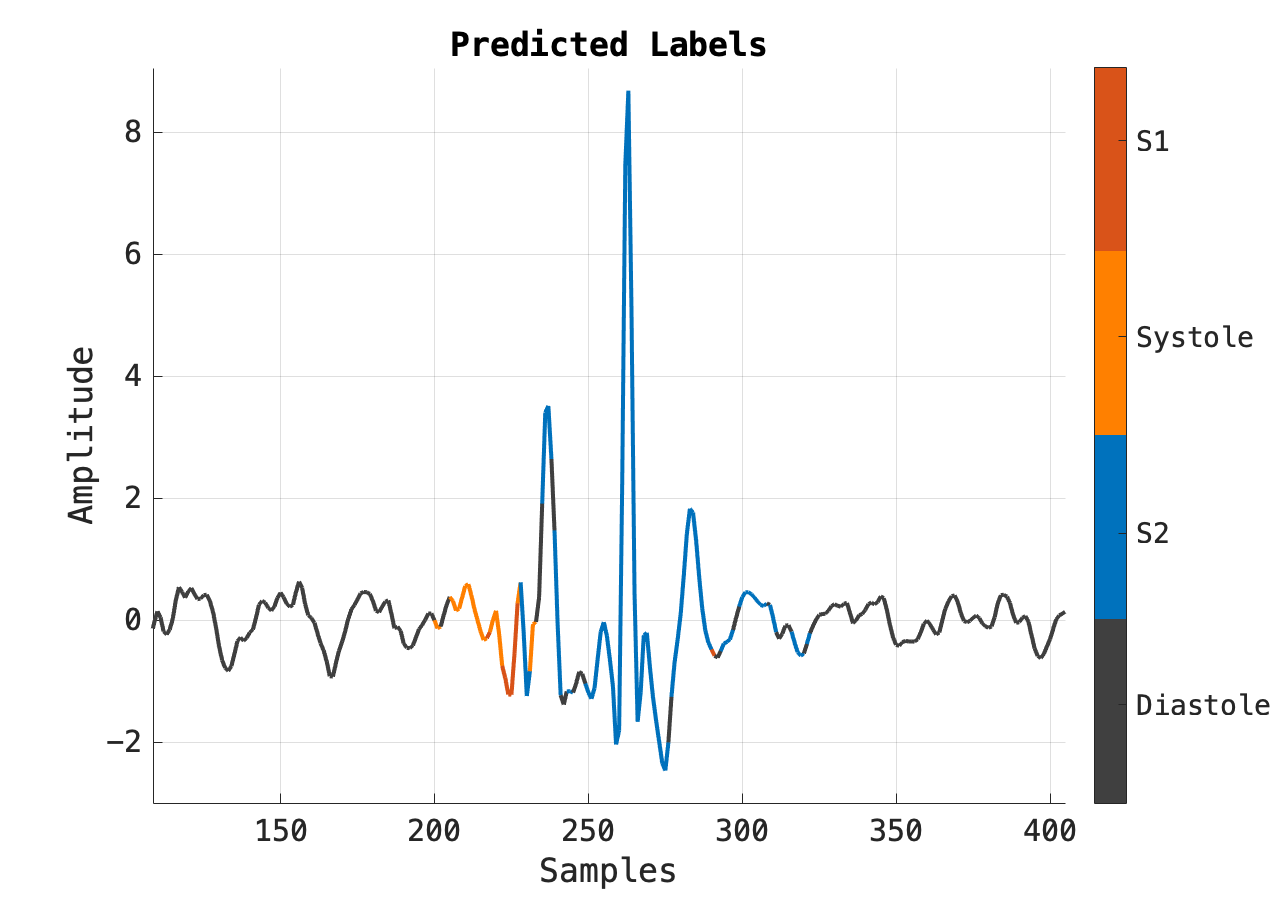
\includegraphics[scale=0.3]{sections/chapter-07/images/predicted-labels.png}
  \caption[Etiquetas predecidas por la red]{Etiquetas predecidas por la red.}
  \label{fig:spurious-transitions}
\end{figure}

\indent Para corregir la transición de estado espúrios los posteriores capítulos se propondrán algunas técnicas.
Esto ayudará a la efectividad de la detección y para mantener la consistencia de los estados. Este ruido no es
deseado en algoritmos que utilicen las transiciones del fonocardiograma.

  \chapter{Discusión}

\section{Resultados}

\indent Ya se ha mencionado la necesidad de realizar comparaciones con diferentes algoritmos que tratan de resolver el problema de segmentación de fonocardiogramas a través de un entrenamiento supervisado con diferentes modelos como han de ser redes neuronales convolucionales y cadenas ocultas de Markov, entre otros. \bigskip

\indent Los resultados se ilustran en los siguientes cuadros donde se ha aplicado la técnica \textit{10-Folds} para cada estado y luego se ha promediado entre todos ellos. La cantidad de atributos extraídos para el entrenamiento ha sido de 44 para un set de datos de 734, 590 y 269 señales tomando segmentos de 2 ms, 3 ms y 5 ms respectivamente. De esta manera la relación de señales-atributos, en el peor caso, es de 6.11 y en el mejor caso, es de 16.68. Esta relación es un índice de generalización del modelo, donde en la literatura y en el campo de la investigación, 10 es el valor mínimo aceptable.

\begin{table}[H]
  \centering
  \begin{tabularx}{\textwidth}{|X|l|l|l|l|l|}
    \hline
    Número de señales & L & $F_1$ & $Acc$ & $P_+$ & $Se$ \\
    \hline
    \thead{269} & \thead{5 ms} & \thead{$\textcolor{gray}{87.3 \pm 3.2}$ \\ $81.4 \pm 4.0$} & \thead{$\textcolor{gray}{95.6 \pm 2.0}$ \\ $93.5 \pm 3.7$} & \thead{$\textcolor{gray}{87.9 \pm 2.2}$ \\ $81.5 \pm 2.5$} & \thead{$\textcolor{gray}{86.6 \pm 2.1}$ \\ $81.4 \pm 2.8$} \\
    \hline
    \thead{590} & \thead{3 ms} & \thead{$\textcolor{gray}{88.6 \pm 3.4}$ \\ $82.4 \pm 3.8$} & \thead{$\textcolor{gray}{96.0 \pm 1.9}$ \\ $93.7 \pm 2.1$} & \thead{$\textcolor{gray}{89.2 \pm 2.2}$ \\ $82.6 \pm 2.9$} & \thead{$\textcolor{gray}{88.0 \pm 1.8}$ \\ $82.2 \pm 2.1$} \\
    \hline
    \thead{734} & \thead{2 ms} & \thead{$\textcolor{gray}{88.2 \pm 2.3}$ \\ $83.7 \pm 2.9$} & \thead{$\textcolor{gray}{95.9 \pm 1.7}$ \\ $94.2 \pm 3.1$} & \thead{$\textcolor{gray}{88.1 \pm 3.4}$ \\ $83.0 \pm 4.1$} & \thead{$\textcolor{gray}{88.3 \pm 2.2}$ \\ $84.5 \pm 2.3$} \\
    \hline
  \end{tabularx}

  \caption[Tabla con las métricas para el sonido 1 (S1)]{Tabla con las métricas para el sonido 1 (S1). L es el largo de la ventana elegida sin solapamiento. $F_1$ es el promedio armónico, \textit{Acc} es la exactitud, $P_+$ es lo que se conoce como precision y Se es la sensibilidad.}

\end{table}

\begin{table}[H]
  \centering
  \begin{tabularx}{\textwidth}{|X|l|l|l|l|l|}
    \hline
    Número de señales & L & $F_1$ & $Acc$ & $P_+$ & $Se$ \\
    \hline
    \thead{269} & \thead{5 ms} & \thead{$\textcolor{gray}{89.6 \pm 3.3}$ \\ $81.4 \pm 3.5$} & \thead{$\textcolor{gray}{95.2 \pm 3.1}$ \\ $92.9 \pm 3.4$} & \thead{$\textcolor{gray}{89.7 \pm 2.3}$ \\ $82.1 \pm 2.7$} & \thead{$\textcolor{gray}{89.6 \pm 2.1}$ \\ $80.7 \pm 2.7$} \\
    \hline
    \thead{590} & \thead{3 ms} & \thead{$\textcolor{gray}{90.7 \pm 1.4}$ \\ $82.9 \pm 2.2$} & \thead{$\textcolor{gray}{95.7 \pm 2.0}$ \\ $92.1 \pm 2.4$} & \thead{$\textcolor{gray}{91.5 \pm 2.1}$ \\ $83.7 \pm 2.7$} & \thead{$\textcolor{gray}{89.9 \pm 2.9}$ \\ $82.1 \pm 3.1$} \\
    \hline
    \thead{734} & \thead{2 ms} & \thead{$\textcolor{gray}{89.5 \pm 2.6}$ \\ $84.0 \pm 2.9$} & \thead{$\textcolor{gray}{95.2 \pm 1.0}$ \\ $92.6 \pm 1.8$} & \thead{$\textcolor{gray}{90.8 \pm 2.1}$ \\ $85.6 \pm 2.5$} & \thead{$\textcolor{gray}{88.3 \pm 3.2}$ \\ $82.5 \pm 3.5$} \\
    \hline
  \end{tabularx}

  \caption[Tabla con las métricas para el sístole isovolumétrico (Sys)]{Tabla con las métricas para el sístole isovolumétrico (Sys). L es el largo de la ventana elegida sin solapamiento. $F_1$ es el promedio armónico, Acc es la exactitud, $P_+$ es lo que se conoce como precision y Se es la sensibilidad.}

\end{table}

\begin{table}[H]
  \centering
  \begin{tabularx}{\textwidth}{|X|l|l|l|l|l|}
    \hline
    Número de señales & L & $F_1$ & $Acc$ & $P_+$ & $Se$ \\
    \hline
    \thead{269} & \thead{5 ms} & \thead{$\textcolor{gray}{87.4 \pm 3.6}$ \\ $81.4 \pm 3.9$} & \thead{$\textcolor{gray}{96.8 \pm 3.1}$ \\ $95.4 \pm 3.5$} & \thead{$\textcolor{gray}{88.1 \pm 2.7}$ \\ $82.1 \pm 3.0$} & \thead{$\textcolor{gray}{86.7 \pm 2.2}$ \\ $80.7 \pm 2.5$} \\
    \hline
    \thead{590} & \thead{3 ms} & \thead{$\textcolor{gray}{88.8 \pm 1.9}$ \\ $80.1 \pm 2.3$} & \thead{$\textcolor{gray}{97.2 \pm 2.0}$ \\ $95.0 \pm 2.7$} & \thead{$\textcolor{gray}{89.5 \pm 2.9}$ \\ $82.1 \pm 3.1$} & \thead{$\textcolor{gray}{88.2 \pm 3.1}$ \\ $78.2 \pm 3.4$} \\

    \hline
    \thead{734} & \thead{2 ms} &
    \thead{$\textcolor{gray}{88.8 \pm 1.9}$ \\ $83.8 \pm 2.1$} & \thead{$\textcolor{gray}{97.2 \pm 2.1}$ \\ $95.9 \pm 2.2$} & \thead{$\textcolor{gray}{89.7 \pm 2.5}$ \\ $84.5 \pm 3.1$} & \thead{$\textcolor{gray}{87.9 \pm 2.8}$ \\ $83.2 \pm 3.0$} \\
    \hline
  \end{tabularx}

  \caption[Tabla con las métricas para el sonido 2 (S2)]{Tabla con las métricas para el sonido 2 (S2). L es el largo de la ventana elegida sin solapamiento.  $F_1$ es el promedio armónico, Acc es la exactitud, $P_+$ es lo que se conoce como precision y Se es la sensibilidad.}

\end{table}

\begin{table}[H]
  \centering
  \begin{tabularx}{\textwidth}{|X|l|l|l|l|l|}
    \hline
    Número de señales & L & $F_1$ & $Acc$ & $P_+$ & $Se$ \\
    \hline
    \thead{269} & \thead{5 ms} & \thead{$\textcolor{gray}{95.0 \pm 1.7}$ \\ $91.9 \pm 2.1$} & \thead{$\textcolor{gray}{94.9 \pm 2.1}$ \\ $91.6 \pm 2.5$} & \thead{$\textcolor{gray}{94.6 \pm 1.9}$ \\ $90.9 \pm 2.1$} & \thead{$\textcolor{gray}{95.5 \pm 1.5}$ \\ $93.0 \pm 2.1$} \\
    \hline
    \thead{590} & \thead{3 ms} & \thead{$\textcolor{gray}{95.2 \pm 1.3}$ \\ $90.7 \pm 1.9$} & \thead{$\textcolor{gray}{95.1 \pm 2.0}$ \\ $90.2 \pm 2.1$} & \thead{$\textcolor{gray}{94.5 \pm 2.1}$ \\ $89.7 \pm 2.3$} & \thead{$\textcolor{gray}{96.0 \pm 1.5}$ \\ $91.6 \pm 2.0$} \\
    \hline
    \thead{734} & \thead{2 ms} & \thead{$\textcolor{gray}{94.7 \pm 2.6}$ \\ $92.1 \pm 2.9$} & \thead{$\textcolor{gray}{94.6 \pm 1.0}$ \\ $91.8 \pm 1.5$} & \thead{$\textcolor{gray}{93.9 \pm 2.1}$ \\ $91.4 \pm 2.5$} & \thead{$\textcolor{gray}{95.5 \pm 2.9}$ \\ $92.7 \pm 3.2$} \\
    \hline
  \end{tabularx}

  \caption[Tabla con las métricas para la diástole isovolumétrica (Dias)]{Tabla con las métricas para la diástole isovolumétrica (Dias). L es el largo de la ventana elegida sin solapamiento.  $F_1$ es el promedio armónico, Acc es la exactitud, $P_+$ es lo que se conoce como precision y Se es la sensibilidad.}

\end{table}

\begin{table}[H]
  \centering
  \begin{tabularx}{\textwidth}{|X|l|l|l|l|l|}
    \hline
    Número de señales & L & $F_1$ & $Acc$ & $P_+$ & $Se$ \\
    \hline
    \thead{269} & \thead{5 ms} & \thead{$\textcolor{gray}{89.8 \pm 3.1}$ \\ $84.9 \pm 4.3$} & \thead{$\textcolor{gray}{95.6 \pm 0.7}$ \\ $93.3 \pm 1.4$} & \thead{$\textcolor{gray}{90.1 \pm 2.7}$ \\ $85.3 \pm 3.8$} & \thead{$\textcolor{gray}{89.6 \pm 3.6}$ \\ $84.5 \pm 5.0$} \\
    \hline
    \thead{590} & \thead{3 ms} & \thead{$\textcolor{gray}{90.8 \pm 2.7}$ \\ $84.0 \pm 4.0$} & \thead{$\textcolor{gray}{96.0 \pm 0.8}$ \\ $92.8 \pm 1.8$} & \thead{$\textcolor{gray}{91.2 \pm 2.1}$ \\ $84.5 \pm 3.0$} & \thead{$\textcolor{gray}{90.5 \pm 3.2}$ \\ $83.5 \pm 4.9$} \\
    \hline
    \thead{734} & \thead{2 ms} & \thead{$\textcolor{gray}{90.3 \pm 2.6}$ \\ $85.9 \pm 3.6$} & \thead{$\textcolor{gray}{95.7 \pm 1.0}$ \\ $93.6 \pm 1.6$} & \thead{$\textcolor{gray}{90.6 \pm 2.1}$ \\ $86.1 \pm 3.2$} & \thead{$\textcolor{gray}{90.0 \pm 3.2}$ \\ $85.7 \pm 4.1$} \\
    \hline
  \end{tabularx}

  \caption[Tabla con las métricas promediadas del sistema.]{Tabla con las métricas promediadas del sistema. L es el largo de la ventana elegida sin solapamiento.  $F_1$ es el promedio armónico, Acc es la exactitud, $P_+$ es lo que se conoce como precision y Se es la sensibilidad.}

\end{table}

\indent Los resultados muestran que para cada uno de los sonidos las mejores métricas se alcanzan para las señales divididas en cuadros de 3 ms. Sin embargo, dada al desvío que presentan todas ellas, no se puede afirmar definitivamente que aumentando la cantidad de señales y al mismo tiempo reduciendo la longitud de los cuadros se mejore la segmentación. \\
\indent Por otro lado, haciendo una comparación de las métricas inter-sonidos, es posible afirmar que el mejor desempeño se obtiene para el cuarto estado o diástole silenciosa. Diferente son los otros tres estados que tienen similares métricas. Uno de los potenciales motivos que hace al cuarto estado facilmente clasificable, es la diferencia de duración temporal claramente marcada frente a los demás, y a esto se le suma el bajo contenido de frecuencias altas. Esto parece permitirle a la red detectarlo con facilidad. Contrariamente, el sístole silencioso muchas veces contiene ruidos asociados a los dos sonidos fundamentales y su duración es mucho más corta. Asimismo, las duraciones entre los tres estados son similares. Esto da la iniciativa que la noción temporal de los estados es un factor muy importante a la hora de la segmentación. Ya hemos visto que los algoritmos \cite{pp:schmidt2010} y \cite{pp:springer2015} donde aplican algoritmos más tradicionales de estimación utilizan el concepto temporal de los distintos estados alcanzando métricas impresionantes. No es así el caso de técnicas más modernas como es \textit{Deep learning} en \cite{pp:renna2018} que explícitamente no queda definida la duración de los estados. De todos modos superan los algoritmos mencionados anteriormente.


\subsection*{Comparación de algoritmos}

\indent Los algoritmos comparados para mostrar en dónde se encuentra el presente trabajo se ilustran en el Cuadro \ref{tab:performance-comparison}. Estos algoritmo se han probado con el mismo set de datos y diferentes técnicas de procesamiento.

\begin{table}[H]
  \centering
  \begin{tabularx}{\textwidth}{|X|l|l|l|l|}
    \hline
    \backslashbox[61mm]{Algoritmos}{Métricas} & $F_1$ & $Acc$ & $P_+$ & $Se$ \\

    \hline
    \thead{Schmidt \cite{pp:schmidt2010}}        &
    \thead{$93.0 \pm 3.2$} &
    \thead{$87.4 \pm 2.6$} &
    \thead{$93.3 \pm 2.8$} &
    \thead{$92.7 \pm 3.8$} \\

    \hline
    \thead{Springer \cite{pp:springer2015}}       &
    \thead{$94.5 \pm 1.8$} &
    \thead{$89.8 \pm 1.2$} &
    \thead{$94.8 \pm 1.8$} &
    \thead{$94.3 \pm 1.8$} \\

    \hline
    \thead{\acrshort{cnn}+max \cite{pp:renna2018}}        &
    \thead{$\mathbf{95.7 \pm 1.3}$} &
    \thead{$\mathbf{93.7} \pm \mathbf{1.0}$} &
    \thead{$\mathbf{95.7} \pm \mathbf{1.4}$} &
    \thead{$\mathbf{95.7} \pm \mathbf{1.2}$} \\

    \hline
    \thead{\acrshort{lstm}}           &
    \thead{$84.9 \pm 4.3$} &
    \thead{$93.3 \pm 1.4$} &
    \thead{$85.3 \pm 3.8$} &
    \thead{$84.5 \pm 5.0$} \\

    \hline
  \end{tabularx}

  \caption[Tabla comparativa de las métricas entre diferentes arquitecturas y técnicas]{Tabla comparativa de las métricas entre diferentes arquitecturas y técnicas. Las señales son \textit{frames} de 5 ms. La arquitectura de Renna \textit{et. al} logra la mayor performance en términos de segmentación.}
  \label{tab:performance-comparison}

\end{table}


\section{Limitaciones}

\indent Por otro lado, este trabajo no ha abordado por completo todos los aspectos de la implementación. La optimización del algoritmo, la arquitectura, el postprocesamiento de la clasificación y la segmentación en tiempo real son temas que quedan por resolver para lograr mejorar esta técnica.

\subsection*{Post-procesamiento}

\indent En el caso del post-procesamiento pueden aplicar varias técnicas. Éstas tienen relación con dar una restricción de transición de estados. Es decir, que sólo luego de un sonido S$_1$ proceda una sístole silenciosa, y así con el resto de los estados.

\subsubsection*{Modelo temporal secuencial máximo}

\indent Para restringir la transición de los estados se consigue aplicando la ecuación \ref{eq:max-temporal-modeling}.

\begin{align} \label{eq:max-temporal-modeling}
\hat{s}(t) =
\begin{cases}
  \Tilde{s}(t), \quad &\Tilde{s}(t) = \mathrm{mod}(\hat{s}(t-1)+1, 4)\\
  \hat{s}(t-1), \quad &\mathrm{en\;otro\;caso}
\end{cases}
\end{align}

\indent Esta ecuación necesita una semilla donde $\hat{s}(0) = \Tilde{s}(0)$. La principal ventaja de este método es la baja complejidad algorítmica y la posibilidad de aplicarlo en una segmentación en tiempo real.

\subsubsection*{Modelado basado en Cadenas Ocultas de Markov (\acrshort{hmm})}

\indent Estrategias más complejas se pueden aplicar para restringir las posibles transiciones. La idea es utilizar las probabilidades a posteriori que la red provee en la matriz $\mathbf{B}$. En particular, es posible utilizar esas probabilidades en un modelo \acrshort{hmm} que restringue estas transiciones. Este modelo se describe en función de los siguientes parámetros: probabilidad a priori de los estados $\pi$, la probabilidad de transiciones de los estados dada por $\gamma_{i,j} = p(s(t)=j|s(t-1)=i)$ y las probabilidades de emisión $e_{t,j} = p(\mathbf{x}(t)|s(t) = j)$. En el caso de $\pi$ y $\gamma_{i,j}$ se pueden estimar mediante el método de Máxima Verosimilitud (\textit{Maximum Likelihood}) a partir de los datos de entrenamiento y sus etiquetas. \\
\indent Por otro lado, las emisiones pueden ser calculadas a partir de la matriz $\mathbf{B}$. Asumiendo que representan una buena aproximación de la probabilidad a posteriori en el tiempo $t$ dada la observación del vector de emisión $\mathbf{x}(t)$.

\begin{align}
  p(s(t) = j | \mathbf{x}(t)) \sim B_{t,j}
\end{align}

\indent Y a través del Teorema de Bayes, es posible computar dichas probabilidades.

\begin{align}
  e_{t,j} = p(\mathbf{x}(t)|s(t)=j) = \frac{p(s(t) = j|\mathbf{x}(t)) \cdot p(\mathbf{x}(t))}{p(s(t) = j)}
\end{align}

\indent En este caso la distribución $p(\mathbf{x}(t))$ es aproximada por una gaussiana multivariable cuya media y matriz de covarianza son estimados a partir de los datos de entrenamiento usando ML. \\
\indent Luego, el modelo \acrshort{hmm} se encarga de determinar la sequencia de estados asociada que maximimiza la función de verosimilitud mediante el algoritmo de Viterbi.

\begin{align}
  \mathcal{L}(s,\mathbf{x}) = p(s(0),\dots,s(n-1),\mathbf{x}(0),\dots,\mathbf{x}(n-1))
\end{align}

\indent De esta manera la sequencia $\hat{s}(t)$ se consigue a partir de la secuencia que maximiza la función de verosimilitud.

\subsubsection*{Modelado basado en Cadenas Ocultas de Markov dependientes del tiempo (\acrshort{dhmm})}

\indent Las probabilidades de emisiones del método anterior, también son utilizadas en este. Además, se introduce la dependencia del tiempo en donde se modela al tiempo en un estado como una distribución gaussiana donde su media y varianza es estimada a partir de un análisis de autocorrelación explicado en \cite{pp:schmidt2010}. Una vez más a partir del algoritmo de Viterbi se decodifica la secuencia $\hat{s}(t)$.

\subsubsection*{Modelado adaptativo basado en Cadenas Ocultas de Markov dependientes del tiempo}

\indent Nuevamente las probabilidades de emisión se utilizan en este método. La distribución de los tiempos en un estado siguen siendo gaussianas, sin embargo las medias y varianzas se computan con el método explicado en \cite{pp:oliveira-renna-coimbra} a partir de la información del \acrshort{pcg}. Así se estiman los parámetros que mejor se adaptan al \acrshort{pcg} a partir de la maximización de una función de verosimilitud incompleta asociada a la secuencia $\mathbf{x}(t)$, $t=0,1,\dots,T-1$. Por supuesto, la secuencia $\hat{s}(t)$ es estimada por Viterbi.
  \chapter{Conclusiones generales}

\indent Este trabajo muestra que la correcta selección de atributos adecuado, acompañado de un modelo relativamente
simple en la etapa de clasificación, alcanza para obtener una efectividad muy cercana a la del estado del arte. En
el cuadro \ref{tab:performance-comparison} se ve que, entre los cuatro algoritmos más famosos en la segmentación de
\acrshort{pcg}, el de F. Renna y M. Coimbra \cite{pp:renna2018} obtiene las mejores métricas. Éste se basa en el
mismo preprocesamiento (acondicionamiento de la señal) y extracción de atributos de los \acrshort{pcg} que Springer
\textit{et al.} \cite{pp:springer2015}, el cual utiliza los métodos propuestos por Schmidt \cite{pp:schmidt2010}
mejorando algunos de los algoritmos. \\
\indent El presente trabajo utiliza, una DNN con una arquitectura muy simple.
Ésta, se ha visto, que contiene sólo una capa recurrente \acrshort{lstm} y diferentes capas intermedias que ayudan a
la clasificación. De esta manera, se alcanzan métricas muy cercanas al estado del arte con una buena elección de
atributos. En cuanto a la exactitud ($Acc$) queda en segundo lugar pero carece de eficiencia en el resto de las
métricas, precisión ($P_+$) y sensibilidad $Se$. \\
\indent La arquitectura de la red \acrshort{lstm} es relativamente simple en comparación con otras arquitecturas,
por ejemplo U-Net, de caracter convolucional, donde se aplican mayores grados de profundidad en cuanto a las capas.
Por otro lado, posee antecedentes en cuanto a la aplicación de distintos problemas de segmentación. Un ejemplo es el
conteo de células, detección y morfometría por medio de imágenes.

\section{Tiempo de procesamiento}

\indent Dado que \textit{Deep learning} se encuentra basado en conexionismo: cuando una neurona o unidad en un
modelo de \textit{Machine learning} no es inteligente, un conjunto de neuronas pueden demostrar un comportamiento lo
suficientemente inteligente para ciertas aplicaciones. Es importante enfatizar que el número de neuronas debe ser
grande para realizar tareas complejas. El tamaño de las redes neuronales han crecido exponencialmente, aunque se
comparan con el tamaño del sistema nervioso central de insectos. Por lo tanto, debido a que el tamaño de las redes
neuronales es crítico, requiere un alto desempeño en cuanto a hardware y software. \\
\indent En definitiva la implementación de los algoritmos, el hardware y el contexto en el que se desea llevar la
aplicación imponen restricciones en el tiempo de procesamiento.

\subsection*{Implementaciones en CPU}

\indent En un principio el entrenamiento y la evaluación de las redes neuronales se diseñaban para un único CPU. Hoy
en día esto no es suficiente. En este trabajo no se prioriza el tiempo de procesamiento, con lo cual la etapa de
entrenamiento que depende de muchos factores, como han de ser la cantidad de datos de entrada y la arquitectura de
la red. Generalmente, la mayoría de estos modelos son utilizados en GPU. Sin embargo, con un cuidado
desarrollo e implementación se pueden lograr mejores tiempos de ejecución con implementaciones en CPU.

\subsection*{Implementaciones en GPU}

\indent Para el desarrollo de los algoritmos de clasificación, por ejemplo de este trabajo y para la implementación
en tiempo real, utilizar GPU acelera el tiempo de procesamiento. Las GPU, hardware especializado que permite
realizar multiplicación de matrices y división en paralelo, se diferencian de las CPU que para realizar tareas en
paralelo es necesario utilizar lo que se conoce como \textit{branching}.

\subsection*{Compresión}

\indent La compresión del modelo es una ventaja ante la limitante de memoria y tiempos de lectura y evaluación. Es
el caso de utilizar la idea de este trabajo en una suerte de producto en tiempo real donde se considera el tiempo de
evaluación mucho más importante que el tiempo de entrenamiento. Esto se debe a que el desarrollador tiene mucho más
recursos para realizar las etapas de entrenamiento y evaluación. Asimismmo, aunque sólo sea necesario entrenar el
modelo una única vez e implementarlo para su uso, el usuario cuenta con cómputo más barato y menos performante.
Aquí, es cuando la compresión del modelo juega un papel muy importante a la hora de llevar a producción una
implementación.

\section{Futuras líneas de trabajo}

\subsection*{Nuevas bases de datos}

\indent La base de datos es un asunto bastante crítico en cuanto a la generalización de los modelos. Aumentar la
cantidad de registros de fonocardiograma con sus anotaciones asociadas es un factor clave para desarrollar aún más
la propuesta de este trabajo y muchos otros también. Junto al dispositivo que el \acrshort{iam} del
\acrshort{conicet} se encuentra desarrollando, será posible acceder a adquisiciones de nuevas señales. Por otro
lado, ligado con la arquitectura de la red, sería una buena línea de trabajo obtener una base de datos basadas en
imágenes tiempo-frecuencia \footnote{Algunos ejemplos de transformaciones que logran esto son la \acrshort{stft},
\acrshort{fsst}, \acrshort{cwt}/\acrshort{dwt}}.

\subsection*{Mejoras en la arquitectura}

\indent La arquitectura es una de las principales limitaciones que resultan de este trabajo. En la arquitectura
presentada sólo consta con un único nivel de profundidad, lo que hace una primera versión de arquitectura muy simple
pero con un gran desempeño. Esta genera la pregunta de cuál sería la eficiencia de un modelo recurrente con una
profundidad mucho mayor. \\
\indent Una buena línea de investigación, para obtener mejores métricas, es la arquitectura donde sería bueno
aumentar la profundidad del modelo con otras capas recurrentes o convolucionales. Para lo último es necesario
aplicar transformaciones a los tensores para que sean compatibles entre sí. Distintos trabajos han demostrado
conseguir eficiencias altas gracias a la complejidad de los modelos. Casos como las arquitecturas de AlexNet
\cite{pp:alexnet} y GoogleNet \cite{pp:googlenet} han mejorado distintas aplicaciones como son aplicaciones de
\textit{Computer Vision} y reconocimiento de imágenes, entre otras.

\subsection*{Complejidad algorítmica}

\indent La complejidad algorítmica de las redes neuronales es un tema de discusión que se encuentra ligada
generalmente al algoritmo utilizado para resolver la estimación de los parámetros de la arquitectura. Algunos
ejemplos de estos algoritmos son \textit{Adam} y \textit{RMSProp}. Por supuesto que además depende de la profundidad
y de la naturaleza de las redes. Por ende, ésta es una línea de trabajo importante para definir los tiempos de
entrenamiento y evaluación del modelo.

\subsection*{Segmentación en tiempo real}

\indent Después de tener definido varios de los problemas mencionados anteriormente, es factible pensar en una
implementación de segmentación en tiempo real. Los temas más críticos para llevar a cabo esto son la elección de la
implementación de la red (bajo CPU o GPU), la arquitectura y la complejidad algorítmica y los tiempos asociados. \\
\indent La segmentación en tiempo real requiere definir lo que se conoce como \textit{pipeline} donde a partir de un
\textit{stream} de datos que ingresa al mismo y se realizan distintas etapas de procesamiento (acondicionamiento,
preprocesamiento, procesamiento, post-procesamiento). Para ellos es necesario bajo ciertos requerimientos del
segmentador online definir los tiempos alcanzables en cada instancia del \textit{pipeline}. Esta no es una tarea
trivial y requiere una investigación previa o acompañada de las distintas líneas de trabajo antes mencionada.

  \afterpage{\null\newpage}
  \listoffigures
  \listoftables
  \afterpage{\null\newpage}
  \begin{thebibliography}{9}
  \bibitem{pp:keith_flack}
  A. Keith and M. Flack. \textit{"The form and nature of the muscular connections between the primary divisions of the
  vertebrate"}. Apr, 4. 1907.
  \bibitem{pp:liang}
  H. Liang, S. Lukkarinen, and I. Hartimo, \textit{“Heart Sound Segmentation Algorithm based on heart sound
  Envelogram”}, in Computers in Cardiology, vol. 24, Lund, Swed, 1997, pp. 105–108.
  \bibitem{pp:liang2}
  H. Liang, L. Sakari, and H. Iiro, \textit{“A Heart Sound Segmentation algorithm using Wavelet Decomposition and
  Reconstruction”} in Proceedings of the 19th Annual International Conference of the IEEE Engineering in Medicine and
  Biology Society, vol. 4, Chicago, IL, USA, 1997, pp. 1630–1633.
  \bibitem{bk:boron3ed}
  Boron, W. F. and Boulpaep E. L. \textit{Fisiología Médica}, 3.$^a$ ed. 2017 Elsevier España, S.L.U.
  \bibitem{pp:hochreiter-schmidhuber}
  S. Hochreiter and J. Schmidhuber. \textit{"Long short-term memory. Neural Computation"}, 9(8):1735–1780, 1997.
  \bibitem{pp:martinez2004}
  J. P. Martínez, R. Almeida, S. Olmos, A. P. Rocha, P. Laguna. \textit{"Wavelet-Based ECG Delineator: Evaluation on
  Standard Databases"}. Apr, 2. 2004.
  \bibitem{pp:schmidt2010}
  S. E Schmidt, C. Holst-Hansen, C. Graff, E. Toft and JJ. Struijk. \textit{"Segmentation of Heart Sound recordings by
  a Duration-dependent Hidden Markov model"}. Jan, 22. 2010.
  \bibitem{pp:zhang2011}
  X. J.  Hu,  J. W Zhang  G. T Cao,  H.H Zhu,  H. Li. \textit{"Feature Extraction and Choice in PCG based on Hilbert
  Transfer"}. Dec, 12. 2011.
  \bibitem{pp:abbas2014}
  A. Abbas, R. Bassam and R. Mazin. \textit{"Automated Pattern Classification for PCG Signal based on Adaptive
  Spectral K-means Clustering Algorithm"}. Mar, 15. 2014.
  \bibitem{pp:springer2015}
  D. Springer, L. Tarassenki and G. Clifford. \textit{Logistic Regression-HSMM-based Heart Sound Segmentation}. Sep, 1
  . 2015.
  \bibitem{pp:renna2018}
  F. Renna and M. Coimbra. \textit{Deep Convolution Neural Netwok for Heart Sound Segmentation}. Jan, 24. 2019.
  \bibitem{ref:logi-regression-springer}
  D. Springer,\textit{"Logistic Regression-HSMM-based Heart Sound Example Code"}, Physionet. 2016.
  \bibitem{ref:illanes-zhang}
  A. Illanes-Manriquez and Q. Zhang, “An algorithm for QRS onset and
  offset detection in single lead electrocardiogram records,” in 29th Annual International Conference of the IEEE
  Engineering in Medicine and Biology Society, Lyon, France, 2007, pp. 541 – 544.
  \bibitem{ref:behar}
  J. Behar, et al., \textit{“A comparison of single channel fetal ecg extraction methods”}, Annals of Biomedical
  Engineering, vol. 42, no. 6, pp. 1340–1353, June 2014.
  \bibitem{ref:behar-oster-clifford}
  J. Behar, J. Oster, and G. D. Clifford, \textit{“Combining and Benchmarking
  Methods of Foetal ECG Extraction Without Maternal or Scalp Electrode Data”}, Physioogical Measurement, vol. 35, no.
  8, pp. 1569–1589, Aug. 2014.
  \bibitem{ref:zhang}
  Q. Zhang, et al., \textit{“An algorithm for robust and efficient location of T wave ends in electrocardiograms”}.
  IEEE Transactions on Biomedical Engineering, vol. 53, no. 12 (Pt 1), pp. 2544–52, Dec. 2006.
  \bibitem{ref:seisdedos}
  C. R. Vázquez-Seisdedos, et al., \textit{“New approach for T-wave end detection on electrocardiogram: performance
  in noisy conditions”}. Biomedical Engineering Online, vol. 10, no. 1, p. 77, Jan. 2011.
  \bibitem{ref:messer}
  S. R. Messer, J. Agzarian, and D. Abbott, “Optimal wavelet denoising for phonocardiograms,” Microelectronics
  Journal, vol. 32, no. 12, pp. 931–941, Dec. 2001.
  \bibitem{ref:kumar}
  D. Kumar, et al., “Noise detection during heart sound recording using periodicity signatures.” Physiological
  Measurement, vol. 32, no. 5, pp. 599–618, May 2011.
  \bibitem{ref:oskiper-watrous}
  T. Oskiper and R. Watrous, “Detection of the first heart sound using a time-delay neural network,” in Computers in
  Cardiology. Memphis, TN, USA: IEEE, 2002, pp. 537–540.
  \bibitem{ref:ergen-tatar-gulcur}
  B. Ergen, Y. Tatar, and H. O. H. Gulcur, “Time-frequency analysis of phonocardiogram signals using wavelet
  transform: a comparative study,” Computer Methods in Biomechanics and Biomedical Engineering, no. October, pp.
  37–41, Jan. 2011.
  \bibitem{ref:liang-sakari-iiro}
  H. Liang, L. Sakari, and H. Iiro, “A heart sound segmentation algorithm using wavelet decomposition and
  reconstruction,” in Proceedings of the 19th Annual International Conference of the IEEE Engineering in Medicine and
  Biology Society, vol. 4, Chicago, IL, USA, 1997, pp. 1630–1633.
  \bibitem{ref:gupta}
  C. Gupta, et al., “Neural network classification of homomorphic segmented heart sounds,” Applied Soft Computing,
  vol. 7, no. 1, pp. 286–297, Jan. 2007.
  \bibitem{ref:daubechies-maes}
  I. Daubechies and S. Maes, “A nonlinear squeezing of the continuous wavelet transform based on auditory nerve
  models,” Wavelets in Medicine and Biology, pp. 527–546, 1996.
  \bibitem{ref:gabor}
  D. Gabor, “Theory of communication. part 1: The analysis of information,” Journal of I.E.E., vol. 93, no. 26, pp.
  429–441, 1946.
  \bibitem{ref:grossmann-morlet}
  A. Grossmann and J. Morlet, “Decomposition of Hardy functions into square integrable wavelets of constant shape,”
  SIAM journal on mathematical analysis, vol. 15, no. 4, pp. 723–736, 1984.
  \bibitem{ref:gill-gavrieli-intrator}
  D. Gill, N. Gavrieli, and N. Intrator, “Detection and identification of heart sounds using homomorphic envelogram
  and self-organizing probabilistic model,” in Computers in Cardiology, Lyon, France, 2005, pp. 957–960.
  \bibitem{pp:adam}
  Kingma, Diederik, and Jimmy Ba. \textit{\" Adam: A method for stochastic optimization."}, 3rd International
  Conference for Learning Representations, San Diego, 2015.
  \bibitem{pp:oliveira-renna-coimbra}
  J. Oliveira, F. Renna, and M. T. Coimbra, “Adaptive sojourn time HSMM for heart sound segmentation,” IEEE J. Biomed.
  Health Informatics, 2018, early access.
  \bibitem{pp:alexnet}
  A. Krizhevsky, I. Sutskever, G. E. Hinton, \textit{``ImageNet Classification with Deep Convolutional
  Neural Networks``}. ImageNet LSVRC-2010.
  \bibitem{pp:googlenet}
  C. Szegedy, W. Liu, Y. Jia, P. Sermanet, S. Reed, D. Anguelov, D. Erhan, V. Vanhoucke, A. Rabinovich,
  \textit{``Going Deeper with Convolutions``}. CVPR 2015.
\end{thebibliography}

\end{document}
